\newpage
\section{Casi d'uso}
Vengono elencati i casi d'uso ricavati dall'analisi del capitolato C1.

\subsection{Attori}
Di seguito è riportato il diagramma UML che descrive la gerarchia degli attori. Sono sono state individuate 3 tipologie differenti di attori con funzionalità crescenti. Gli attori sono: l'utente non autenticato, l'utente autenticato e l'amministratore API Market (un attore autenticato con alcune funzionalità superuser). Un quarto attore, chiamato utente generico, viene utilizzato nei diagrammi UML per indicare funzionalità fruibili indipendentemente dallo status di autenticazione.

\label{Attori}

\begin{figure}[ht]
	\centering
	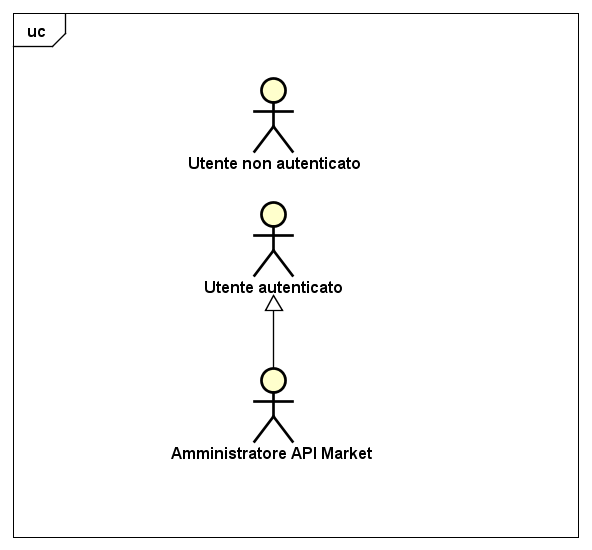
\includegraphics[scale=0.45]{UML/attori.png}
	\caption{Attori}
\end{figure}


\newpage
\subsection{Caso d'uso UC1: Main pre-autenticazione}
\label{UC1}
\begin{figure}[ht]
	\centering
	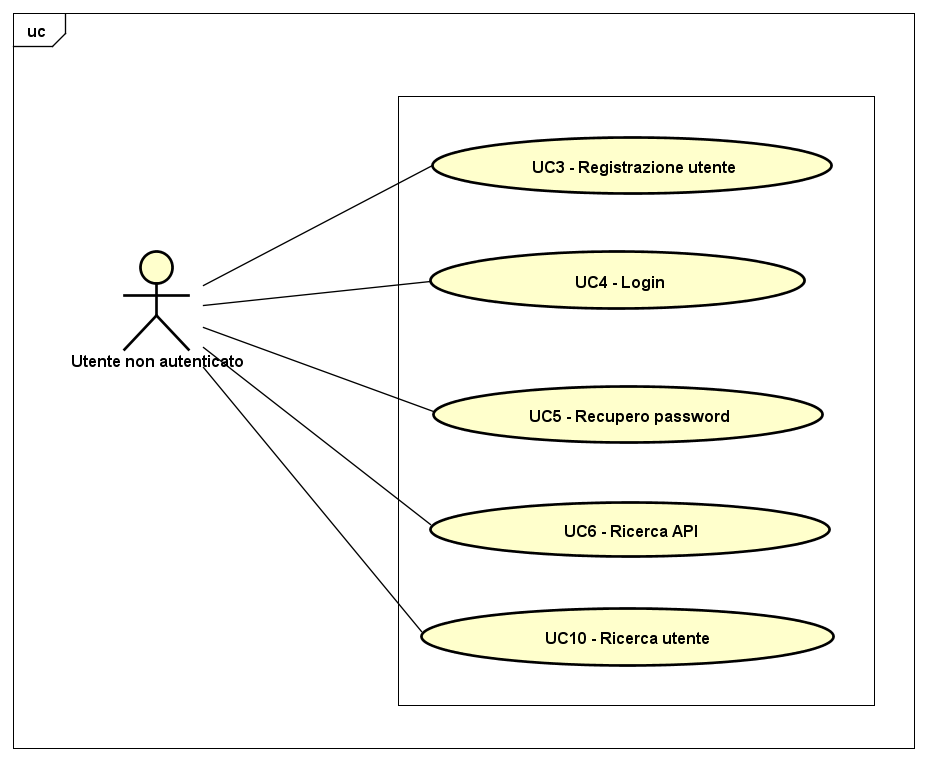
\includegraphics[scale=0.45]{UML/UC1.png}
	\caption{UC1: Main pre-autenticazione}
\end{figure}

\renewcommand*{\arraystretch}{1.6}
\begin{longtable}{ l | p{11cm}}
	\hline
	\rowcolor{Gray}
	\multicolumn{2}{c}{UC1 - Main pre-autenticazione} \\
	\hline
	\textbf{Attori} & Utente non autenticato  \\
	\textbf{Descrizione} & L'attore si trova nella schermata principale dell'applicazione ed accede alle funzionalità a lui disponibili: la registrazione, il login, il recupero password, la ricerca API \\
	\textbf{Pre-Condizioni} & L'attore ha avviato l'applicazione web e non si è ancora autenticato \\
	\textbf{Post-Condizioni} & L'applicazione ha eseguito le richieste dell'attore \\
	\textbf{Scenario Principale} & 
	\begin{enumerate*}[label=(\arabic*.),itemjoin={\newline}]
		\item L'attore può registrarsi all'applicazione (UC3)
		\item L'attore può effettuare il login all'applicazione (UC4)
		\item L'attore può recuperare la propria password (UC5)
		\item L'attore può effettuare una ricerca sulle API presenti nell'applicazione (UC6)
	\end{enumerate*}\\
	\textbf{Scenari Alternativi} & 
	\begin{enumerate*}[label=(\arabic*.),itemjoin={\newline}]
		\item L'attore può effettuare il login tramite API Market (UC4.1)
		\item L'attore può effettuare il login tramite Facebook (UC4.2)
		\item L'attore può effettuare il login tramite Twitter (UC4.3)
		\item L'attore può effettuare il login tramite LinkedIn (UC4.4)
		\item L'attore può effettuare il login tramite Google+ (UC4.5)
	\end{enumerate*}\\
\end{longtable}
\newpage
\subsection{Caso d'uso UC2: Main post-autenticazione }
\label{UC2}
\begin{figure}[ht]
	\centering
	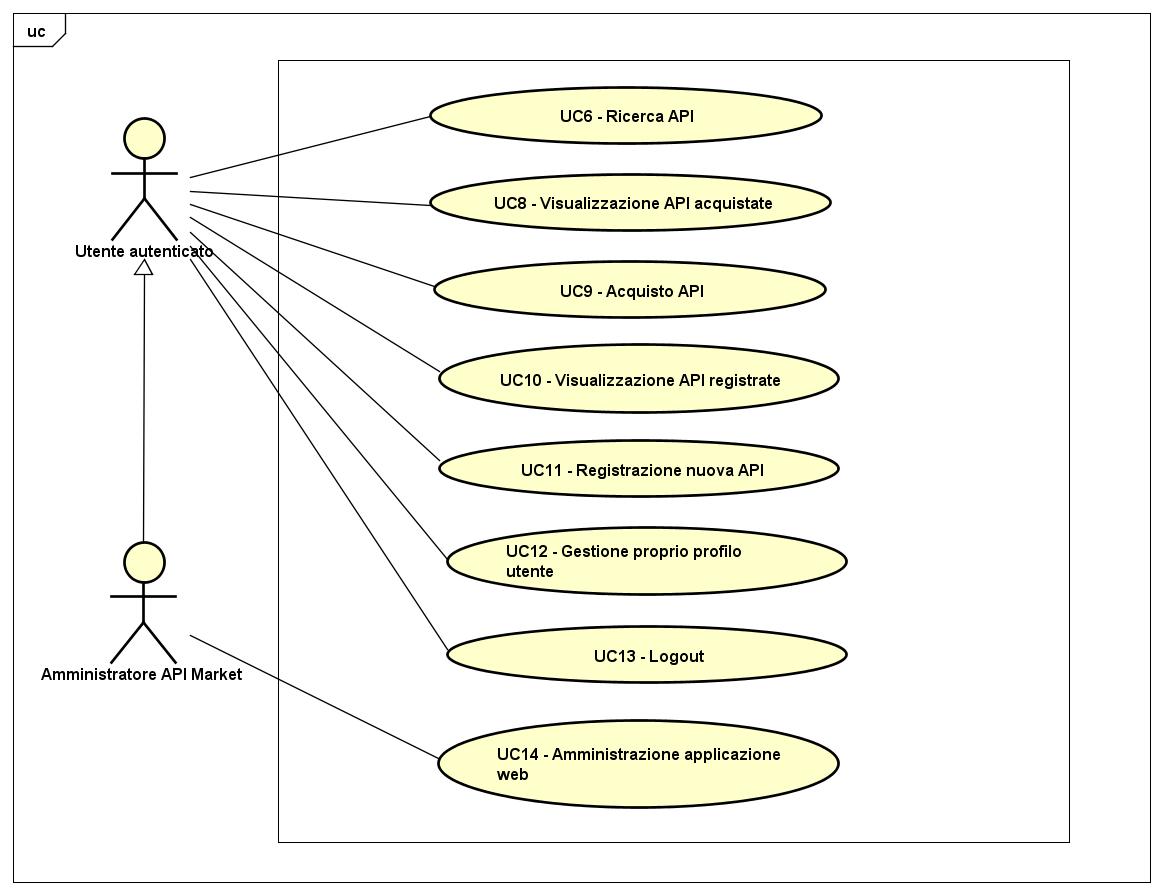
\includegraphics[scale=0.45]{UML/UC2.png}
	\caption{UC2: Main post-autenticazione}
\end{figure}

\begin{longtable}{ l | p{11cm}}
	\hline
	\rowcolor{Gray}
	 \multicolumn{2}{c}{UC2 - Main post-autenticazione} \\
	 \hline
	\textbf{Attori} & Utente autenticato, Amministratore API Market \\
	\textbf{Descrizione} & L'attore tramite la schermata principale
	dell'applicazione, può accedere e sfruttare le funzionalità a lui disponibili: l'interazione
	con il proprio profilo utente, con le API non acquistate e non, con le API registrate, la
	registrazione di una nuova API, il logout. 
	L'Amministratore API Market, oltre alle funzionalità offerte all'utente autenticato, può
	visualizzare i dati di utilizzo delle API ed amministrare l'applicazione web.  \\
	\textbf{Pre-Condizioni} & L'attore ha avviato l'applicazione web e si è autenticato \\
	\textbf{Post-Condizioni} & L'applicazione ha eseguito le richieste dell'attore \\
	\textbf{Scenario Principale} & 
	\begin{enumerate*}[label=(\arabic*.),itemjoin={\newline}]
		\item L'attore può effettuare una ricerca sulle API presenti nell'applicazione
(UC6)
		\item L'attore può visualizzare le API da lui acquistate (UC7)
		\item L'attore può visualizzare le API da lui registrate (UC8)
		\item L'attore può registrare una nuova API (UC9)
		\item L'attore può effettuare una ricerca sugli utenti registrati all'applicazione (UC10)
		\item L'attore può visualizzare il proprio profilo utente (UC11)
		\item L'attore può effettuare il logout (UC12)
		\item L'amministratore API Market può accedere ai servizi di amministrazione dell'applicazione web (UC13)
	\end{enumerate*}\\
\end{longtable}
\newpage
\subsection{Caso d'uso UC3:  Registrazione utente }
\label{UC3}
\begin{figure}[ht]
	\centering
	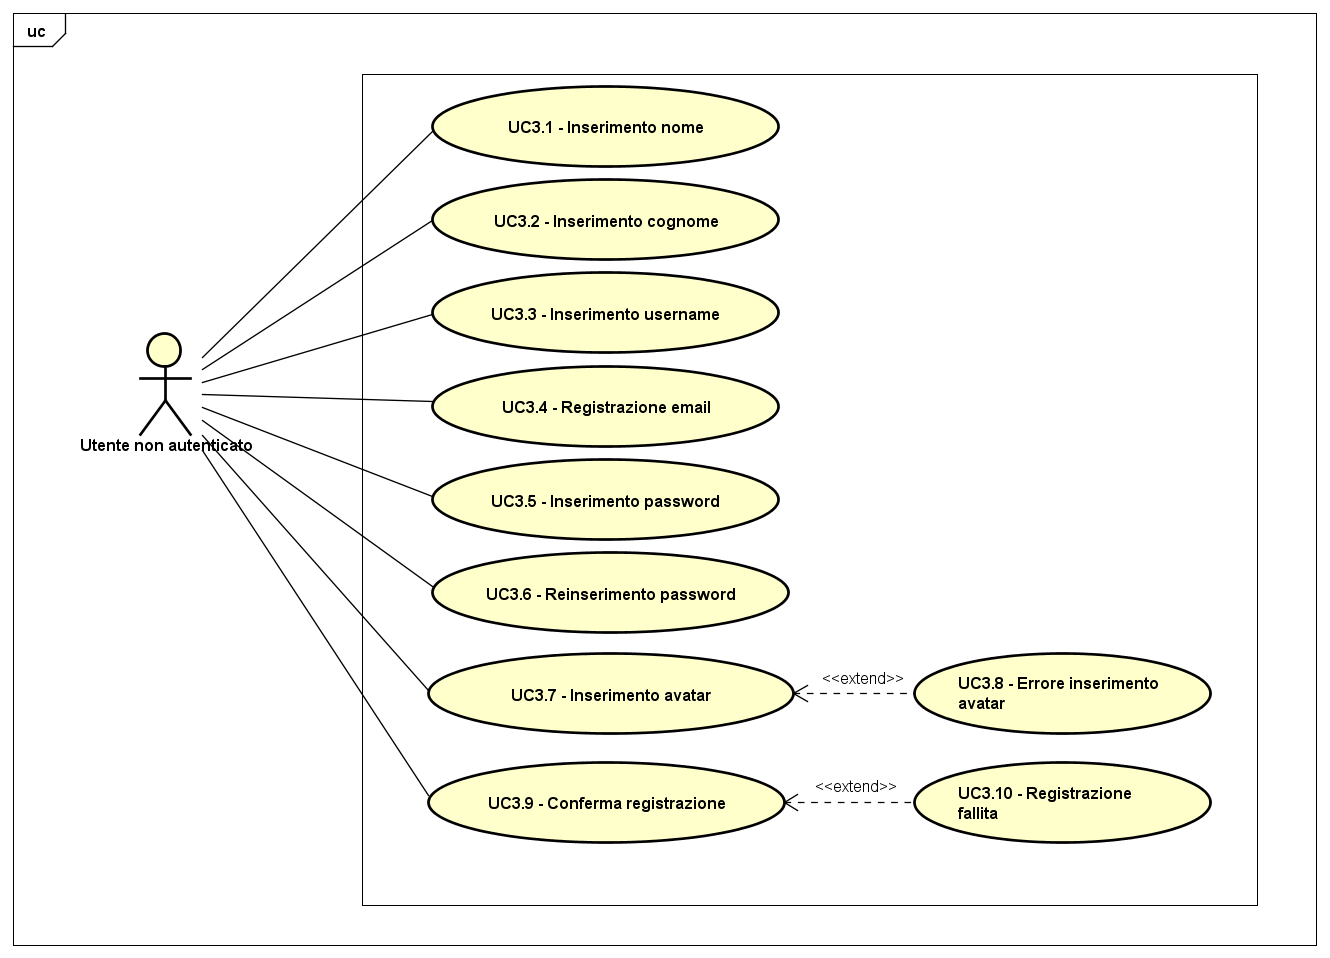
\includegraphics[scale=0.45]{UML/UC3.png}
	\caption{UC3: Registrazione utente}
\end{figure}

\begin{longtable}{ l | p{11cm}}
	\hline
	\rowcolor{Gray}
	 \multicolumn{2}{c}{UC3 - Registrazione utente} \\
	 \hline
	\textbf{Attori} & Utente non autenticato \\
	\textbf{Descrizione} & L'attore inserisce le sue informazioni personali per potersi registrare all'applicazione web, così da poter successivamente effettuare il login ed evolversi in un utente autenticato.
	L'amministratore API Market, oltre alle funzionalità offerte all'utente autenticato, può
	visualizzare i dati di utilizzo delle API ed amministrare l'applicazione web.  \\
	\textbf{Pre-Condizioni} & L'attore ha scelto di registrarsi e l'applicazione web mostra la schermata di registrazione \\
	\textbf{Post-Condizioni} & L'attore si è registrato all'applicazione web \\
	\textbf{Scenario Principale} & \begin{enumerate*}[label=(\arabic*.),itemjoin={\newline}]
		\item L'attore può inserire il proprio nome (UC3.1)
		\item L'attore può inserire il proprio cognome (UC3.2)
		\item L'attore può inserire il proprio username (UC3.3)
		\item L'attore può inserire la propria email (UC3.4) 
		\item L'attore può inserire la propria password (UC3.5)
		\item L'attore può reinserire la propria password per conferma (UC3.6)
		\item L'attore può confermare i dati inseriti, registrandosi all'applicazione web (UC3.7)
	\end{enumerate*}\\
\end{longtable}
\subsubsection{Caso d'uso UC3.1:  Inserimento Nome}
\label{UC3_1}

\begin{longtable}{ l | p{11cm}}
	\hline
	\rowcolor{Gray}
	 \multicolumn{2}{c}{UC3.1 - Inserimento Nome} \\
	 \hline
	\textbf{Attori} & Utente Non Autenticato \\
	\textbf{Descrizione} & L'utente non autenticato inserisce il suo nome  \\
	\textbf{Pre-Condizioni} & L'utente ha scelto di registrarsi e l'applicazione web mostra la schermata di registrazione \\
	\textbf{Post-Condizioni} & L'utente visualizza area per registrazione a applicazione web \\
	\textbf{Scenario Principale} & \begin{enumerate*}[label=(\arabic*.),itemjoin={\newline}]
		\item L'utente non autenticato può inserire il proprio Nome (UC3.1)
	\end{enumerate*}\\
	\textbf{Scenari Alternativi} & 
	\begin{enumerate*}[label=(\arabic*.),itemjoin={\newline}]
		\item Il Nome non e' valido perche' contiene caratteri particolari
	\end{enumerate*}\\
\end{longtable}
\subsubsection{Caso d'uso UC3.2:  Inserimento Cognome}
\label{UC3_2}

\begin{longtable}{ l | p{11cm}}
	\hline
	\rowcolor{Gray}
	 \multicolumn{2}{c}{UC3.2 - Inserimento Cognome} \\
	 \hline
	\textbf{Attori} & Utente Non Autenticato \\
	\textbf{Descrizione} & L'utente non autenticato inserisce il suo Cognome  \\
	\textbf{Pre-Condizioni} & L'utente ha scelto di registrarsi e l'applicazione web mostra la schermata di registrazione \\
	\textbf{Post-Condizioni} & L'utente visualizza area per registrazione a applicazione web \\
	\textbf{Scenario Principale} & \begin{enumerate*}[label=(\arabic*.),itemjoin={\newline}]
		\item L'utente non autenticato può inserire il proprio Cognome (UC3.2)
	\end{enumerate*}\\
	\textbf{Scenari Alternativi} & 
	\begin{enumerate*}[label=(\arabic*.),itemjoin={\newline}]
		\item Il Cognome non e' valido perche' contiene caratteri particolari
	\end{enumerate*}\\
\end{longtable}
\subsubsection{Caso d'uso UC3.3: Inserimento username}
\label{UC3_3}

\begin{longtable}{ l | p{11cm}}
	\hline
	\rowcolor{Gray}
	 \multicolumn{2}{c}{UC3.3: Inserimento username} \\
	 \hline
	\textbf{Attori} & Utente non autenticato \\
	\textbf{Descrizione} & L'attore inserisce lo username desiderato \\
	\textbf{Pre-Condizioni} & L'applicazione mostra il campo dati per l'inserimento dello username \\
	\textbf{Post-Condizioni} & L'attore ha inserito lo username desiderato \\
	\textbf{Scenario Principale} & \begin{enumerate*}[label=(\arabic*.),itemjoin={\newline}]
		\item L'attore può inserire lo username desiderato
	\end{enumerate*}\\
\end{longtable}
\subsubsection{Caso d'uso UC3.4:  Registrazione email}
\label{UC3_4}

\begin{longtable}{ l | p{11cm}}
	\hline
	\rowcolor{Gray}
	 \multicolumn{2}{c}{UC3.4 - Inserimento email} \\
	 \hline
	\textbf{Attori} & Utente non autenticato \\
	\textbf{Descrizione} & L'attore inserisce la propria email  \\
	\textbf{Pre-Condizioni} & L'applicazione visualizza i form per l'inserimento del campo per l'email \\
	\textbf{Post-Condizioni} & L'attore ha inserito la propria email \\
	\textbf{Scenario Principale} & \begin{enumerate*}[label=(\arabic*.),itemjoin={\newline}]
		\item L'utente non autenticato può inserire la propria email
	\end{enumerate*}\\
\end{longtable}

\subsubsection{Caso d'uso UC3.5:  Inserimento Password}
\label{UC3_5}

\begin{longtable}{ l | p{11cm}}
	\hline
	\rowcolor{Gray}
	 \multicolumn{2}{c}{UC3.5 - Inserimento Conferma Password} \\
	 \hline
	\textbf{Attori} & Utente Non Autenticato \\
	\textbf{Descrizione} & L'utente non autenticato inserisce la Password  \\
	\textbf{Pre-Condizioni} & L'utente ha scelto di registrarsi e l'applicazione web mostra la schermata di registrazione \\
	\textbf{Post-Condizioni} & L'utente visualizza area per registrazione a applicazione web \\
	\textbf{Scenario Principale} & \begin{enumerate*}[label=(\arabic*.),itemjoin={\newline}]
		\item L'utente non autenticato può inserire la Password (UC3.5)
	\end{enumerate*}\\
	\textbf{Scenari Alternativi} & 
	\begin{enumerate*}[label=(\arabic*.),itemjoin={\newline}]
		\item La password non e' valida perche' contiene caratteri particolari
		\item La password non e' valida perche' troppo corta
		\item La password non e' valida perche' non contiene almeno un numero
	\end{enumerate*}\\
\end{longtable}
\subsubsection{Caso d'uso UC3.6: Reinserimento password}
\label{UC3_6}

\begin{longtable}{ l | p{11cm}}
	\hline
	\rowcolor{Gray}
	 \multicolumn{2}{c}{UC3.6 - Reinserimento password} \\
	 \hline
	\textbf{Attori} & Utente non autenticato \\
	\textbf{Descrizione} & L'attore reinserisce la password desiderata  \\
	\textbf{Pre-Condizioni} & L'applicazione mostra il campo dati per il reinserimento della password \\
	\textbf{Post-Condizioni} & L'attore ha reinserito la password desiderata \\
	\textbf{Scenario Principale} & \begin{enumerate*}[label=(\arabic*.),itemjoin={\newline}]
		\item L'attore può reinserire la password desiderata
	\end{enumerate*}\\
\end{longtable}
\subsubsection{Caso d'uso UC3.7:  Conferma Inserimenti}
\label{UC3_7}

\begin{longtable}{ l | p{11cm}}
	\hline
	\rowcolor{Gray}
	 \multicolumn{2}{c}{UC3.7 - Conferma Inserimenti} \\
	 \hline
	\textbf{Attori} & Utente Non Autenticato \\
	\textbf{Descrizione} & L'utente non autenticato Conferma i dati inseriti durante la registrazione \\
	\textbf{Pre-Condizioni} & L'utente ha scelto di registrarsi e l'applicazione web mostra la schermata di registrazione \\
	\textbf{Post-Condizioni} & L'utente visualizza un Messaggio di Conferma Registrazione \\
	\textbf{Scenario Principale} & \begin{enumerate*}[label=(\arabic*.),itemjoin={\newline}]
		\item L'utente non autenticato Conferma gli Inserimenti (UC3.7)
	\end{enumerate*}\\
\end{longtable}
\subsubsection{Caso d'uso UC3.8:  Registrazione fallita}
\label{UC3_8}

\begin{longtable}{ l | p{11cm}}
	\hline
	\rowcolor{Gray}
	 \multicolumn{2}{c}{UC3.8 - Registrazione fallita} \\
	 \hline
	\textbf{Attori} & Utente non autenticato \\
	\textbf{Descrizione} & L'attore non si è registrato con successo  \\
	\textbf{Pre-Condizioni} & L'attore ha confermato i dati inseriti \\
	\textbf{Post-Condizioni} & L'attore visualizza i campi dati errati con relativo suggerimento \\
	\textbf{Scenario Principale} & \begin{enumerate*}[label=(\arabic*.),itemjoin={\newline}]
		\item L'attore visualizza i campi dati che non soddisfano i criteri richiesti dalla piattaforma (E.g: Campi dati vuoti, caratteri speciali, username o email già presente etc.)
	\end{enumerate*}\\
\end{longtable}
\newpage
\subsection{Caso d'uso UC4: Login}
\label{UC4}

\begin{longtable}{ l | p{11cm}}
	\hline
	\rowcolor{Gray}
	 \multicolumn{2}{c}{UC4 - Login}\\
	 \hline
	\textbf{Attori} & Utente non autenticato \\
	\textbf{Descrizione} & L'attore inserisce le sue informazioni personali per poter accedere all'applicazione web ed evolversi in un utente autenticato \\
	\textbf{Pre-Condizioni} & L'attore si trova nella schermata iniziale dell'applicazione web \\
	\textbf{Post-Condizioni} & L'attore ha effettuato l'accesso all'applicazione web \\
	\textbf{Scenario Principale} & 
	\begin{enumerate*}[label=(\arabic*.),itemjoin={\newline}]
		\item L'attore può effettuare il login all'applicazione web
	\end{enumerate*}\\
\end{longtable}
\subsubsection{Caso d'uso UC4.1:  Login Base}
\label{UC4_1}
\begin{figure}[ht]
	\centering
	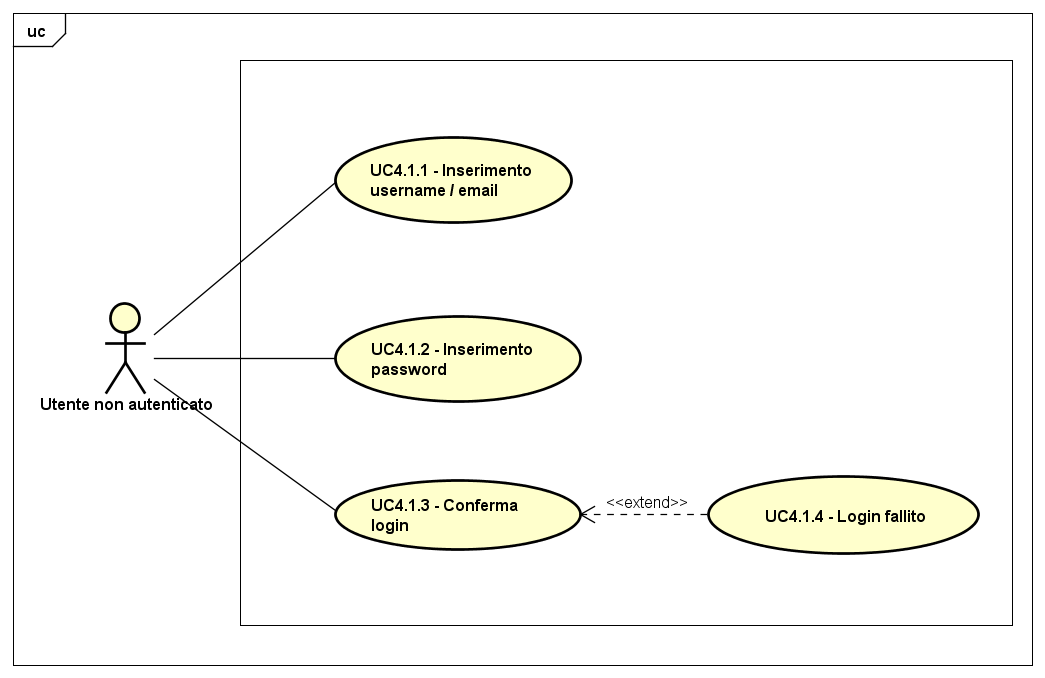
\includegraphics[scale=0.45]{UML/UC4_1.png}
	\caption{UC4.1: Login Base}
\end{figure}

\begin{tabular}{ l | p{11cm}}
	\hline
	\rowcolor{Gray}
	 \multicolumn{2}{c}{UC4.1 - Login Base} \\
	 \hline
	\textbf{Attori} & Utente Non Autenticato \\
	\textbf{Descrizione} & L'utente non autenticato effettua il login all'applicazione web, così da evolversi in un utente autenticato\\
	\textbf{Pre-Condizioni} & L'utente ha scelto di eseguire il login all'applicazione web e non è autenticato \\
	\textbf{Post-Condizioni} & L'utente ha effettuato il login all'applicazione web, evolvendosi in un utente autenticato \\
	\textbf{Scenario Principale} & 
	\begin{enumerate*}[label=(\arabic*.),itemjoin={\newline}]
		\item L'utente non autenticato può inserire l'email o username(UC4.1.1)
		\item L'utente non autenticato può inserire la password(UC4.1.2)
		\item L'utente non autenticato può confermare i dati per loggarsi(UC4.1.3)
	\end{enumerate*}\\
		\textbf{Scenari Alternativi} & 
	\begin{enumerate*}[label=(\arabic*.),itemjoin={\newline}]
		\item L'utente non autenticato visualizza un errore dovuto a un mismatch dei dati immessi e il login non avviene (UC4.1.4)
	\end{enumerate*}\\
\end{tabular}
\subsubsection{Caso d'uso UC4.2:  Login Tramite Facebook }
\label{UC4_2}
\begin{figure}[ht]
	\centering
	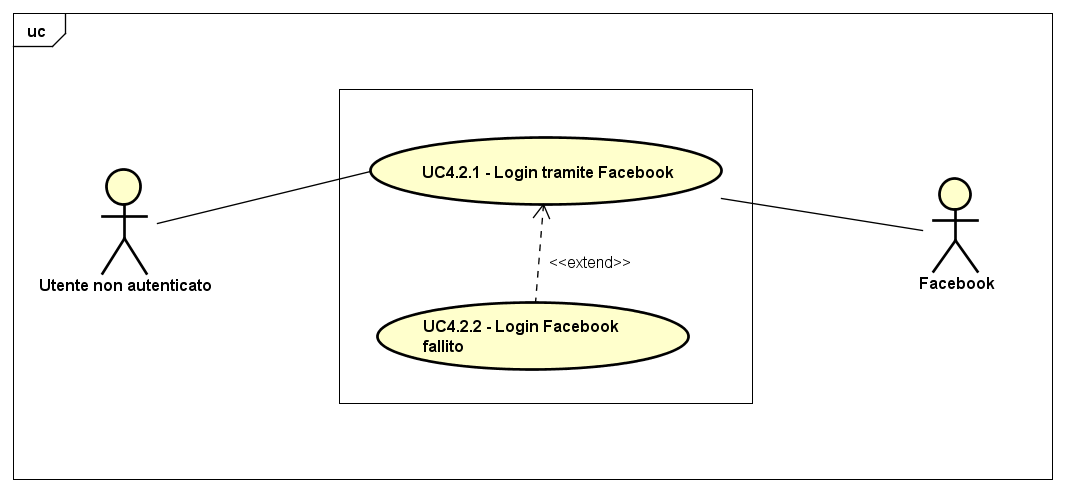
\includegraphics[scale=0.45]{UML/UC4_2.png}
	\caption{UC4.2: Login Tramite Facebook}
\end{figure}

\begin{tabular}{ l | p{11cm}}
	\hline
	\rowcolor{Gray}
	 \multicolumn{2}{c}{UC4.2 - Login Tramite Facebook} \\
	 \hline
	\textbf{Attori} & Utente Non Autenticato, Facebook \\
	\textbf{Descrizione} & L'utente non autenticato effettua il login all'applicazione web tramite Facebook, così da evolversi in un utente autenticato\\
	\textbf{Pre-Condizioni} & L'utente ha scelto di eseguire il login all'applicazione web e non è autenticato \\
	\textbf{Post-Condizioni} & L'utente ha effettuato il login all'applicazione web tramite Facebook, evolvendosi in un utente autenticato \\
	\textbf{Scenario Principale} & \begin{enumerate*}[label=(\arabic*.),itemjoin={\newline}]
		\item L'utente non autenticato può effettuare il login all'applicazione web tramite Facebook (UC4.2.1)
	\end{enumerate*}\\
\end{tabular}
\newpage
\subsubsection{Caso d'uso UC4.3: Login tramite Twitter }
\label{UC4_3}
\begin{figure}[!htbp]
	\centering
	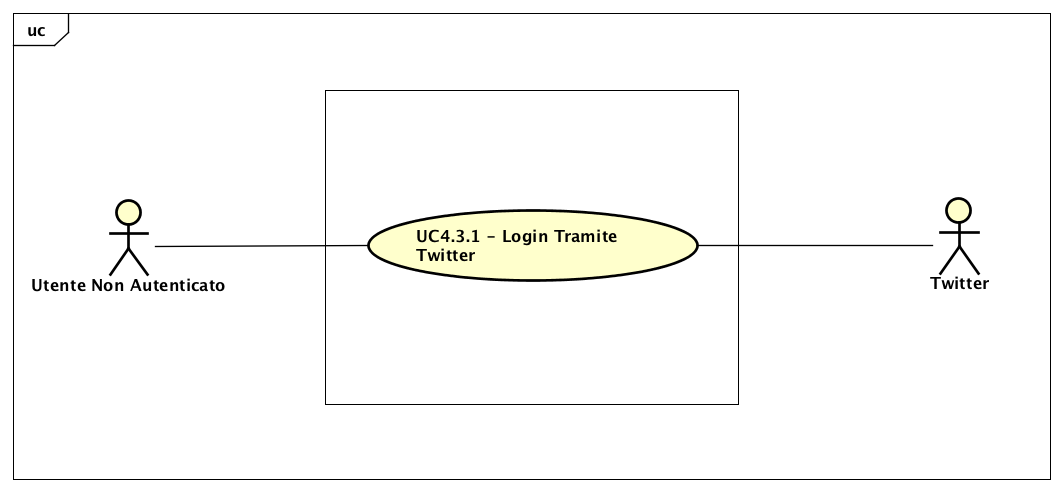
\includegraphics[scale=0.45]{UML/UC4_3.png}
	\caption{UC4.3: Login tramite Twitter}
\end{figure}

\begin{tabular}{ l | p{11cm}}
	\hline
	\rowcolor{Gray}
	\multicolumn{2}{c}{UC4.3 - Login tramite Twitter} \\
	\hline
	\textbf{Attori} & Utente non autenticato, Twitter \\
	\textbf{Descrizione} & L'attore effettua il login all'applicazione web tramite Twitter, così da evolversi in un utente autenticato \\
	\textbf{Pre-Condizioni} & L'attore ha scelto di eseguire il login all'applicazione web tramite Twitter (e non è autenticato) \\
	\textbf{Post-Condizioni} & L'attore ha effettuato il login all'applicazione web tramite Twitter, evolvendosi in un utente autenticato \\
	\textbf{Scenario Principale} & \begin{enumerate*}[label=(\arabic*.),itemjoin={\newline}]
		\item L'attore può effettuare con successo il login tramite Twitter (UC4.3.1), visualizzando un messaggio di successo, e venendo reindirizzato alla pagina principale evolvendosi in un utente autenticato (UC2)
	\end{enumerate*}\\
	\textbf{Scenari Alternativi} & \begin{enumerate*}[label=(\arabic*.),itemjoin={\newline}]
	\item L'attore ha fallito il login tramite Twitter (E.g: Mancanza di privilegi/autorizzazioni, problemi legati a Twitter...) e visualizza un messaggio d'errore (UC4.3.2)
	\end{enumerate*}\\
\end{tabular}
\newpage
\subsubsection{Caso d'uso UC4.4: Login tramite LinkedIn }
\label{UC4_2}
\begin{figure}[!htbp]
	\centering
	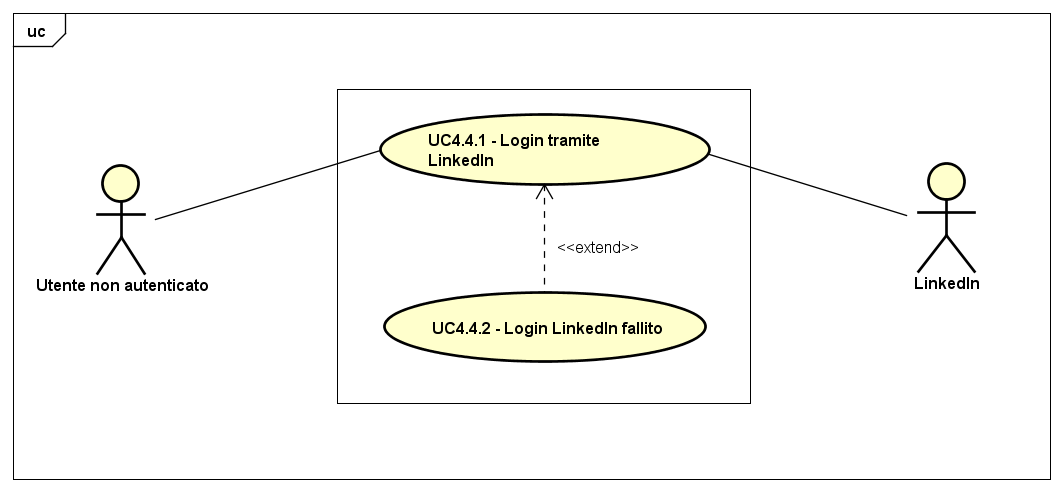
\includegraphics[scale=0.45]{UML/UC4_4.png}
	\caption{UC4.2: Login tramite LinkedIn}
\end{figure}

\begin{tabular}{ l | p{11cm}}
	\hline
	\rowcolor{Gray}
	\multicolumn{2}{c}{UC4.4 - Login tramite LinkedIn} \\
	\hline
	\textbf{Attori} & Utente non autenticato, LinkedIn \\
	\textbf{Descrizione} & L'attore effettua il login all'applicazione web tramite LinkedIn, così da evolversi in un utente autenticato \\
	\textbf{Pre-Condizioni} & L'attore ha scelto di eseguire il login all'applicazione web tramite LinkedIn (e non è autenticato) \\
	\textbf{Post-Condizioni} & L'attore ha effettuato il login all'applicazione web tramite LinkedIn, evolvendosi in un utente autenticato \\
	\textbf{Scenario Principale} & \begin{enumerate*}[label=(\arabic*.),itemjoin={\newline}]
		\item L'attore può effettuare con successo il login tramite LinkedIn (UC4.4.1), visualizzando un messaggio di successo, e venendo reindirizzato alla pagina principale evolvendosi in un utente autenticato (UC2)
	\end{enumerate*}\\
	\textbf{Scenari Alternativi} & \begin{enumerate*}[label=(\arabic*.),itemjoin={\newline}]
	\item L'attore ha fallito il login tramite LinkedIn (E.g: Mancanza di privilegi/autorizzazioni, utente non correttamente loggato a LinkedIn...) e visualizza un messaggio d'errore (UC4.4.2)
	\end{enumerate*}\\
\end{tabular}

\subsubsection{Caso d'uso UC4.5: Login Tramite Google+ }
\label{UC4_5}
\begin{figure}[ht]
	\centering
	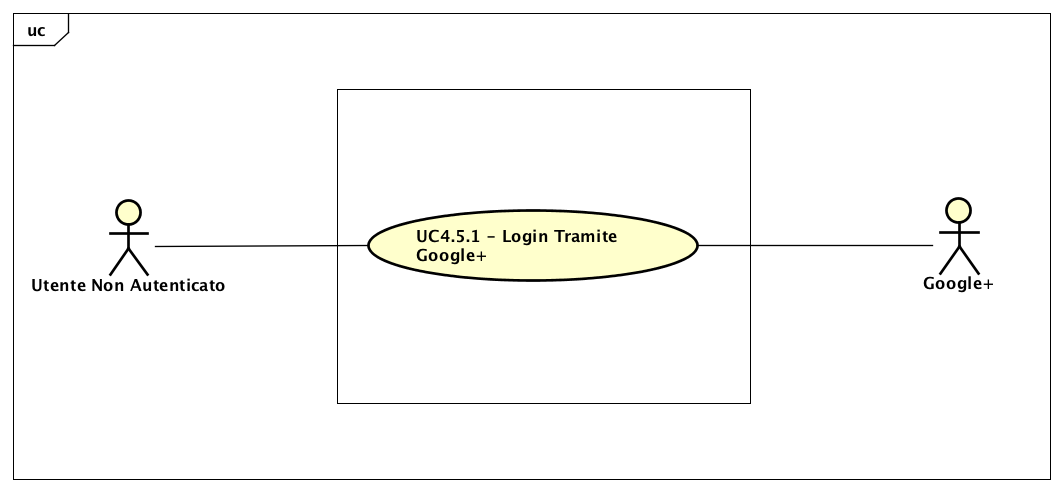
\includegraphics[scale=0.45]{UML/UC4_5.png}
	\caption{UC4.5: Login Tramite Google+ }
\end{figure}

\begin{longtable}{ l | p{11cm}}
	\hline
	\rowcolor{Gray}
	 \multicolumn{2}{c}{UC4.5 - Login Tramite Google+} \\
	 \hline
	\textbf{Attori} & Utente Non Autenticato, Google+ \\
	\textbf{Descrizione} & L'utente non autenticato effettua il login all'applicazione web tramite Google+, così da evolversi in un utente autenticato\\
	\textbf{Pre-Condizioni} & L'utente ha scelto di eseguire il login all'applicazione web e non è autenticato \\
	\textbf{Post-Condizioni} & L'utente ha effettuato il login all'applicazione web tramite Google+, evolvendosi in un utente autenticato\\
	\textbf{Scenario Principale} & \begin{enumerate*}[label=(\arabic*.),itemjoin={\newline}]
		\item L'utente non autenticato può effettuare il login all'applicazione web tramite Google+ (UC4.5.1)
	\end{enumerate*}\\
\end{longtable}
\newpage
\subsection{Caso d'uso UC5: Recupero password}
\label{UC5}
\begin{figure}[ht]
	\centering
	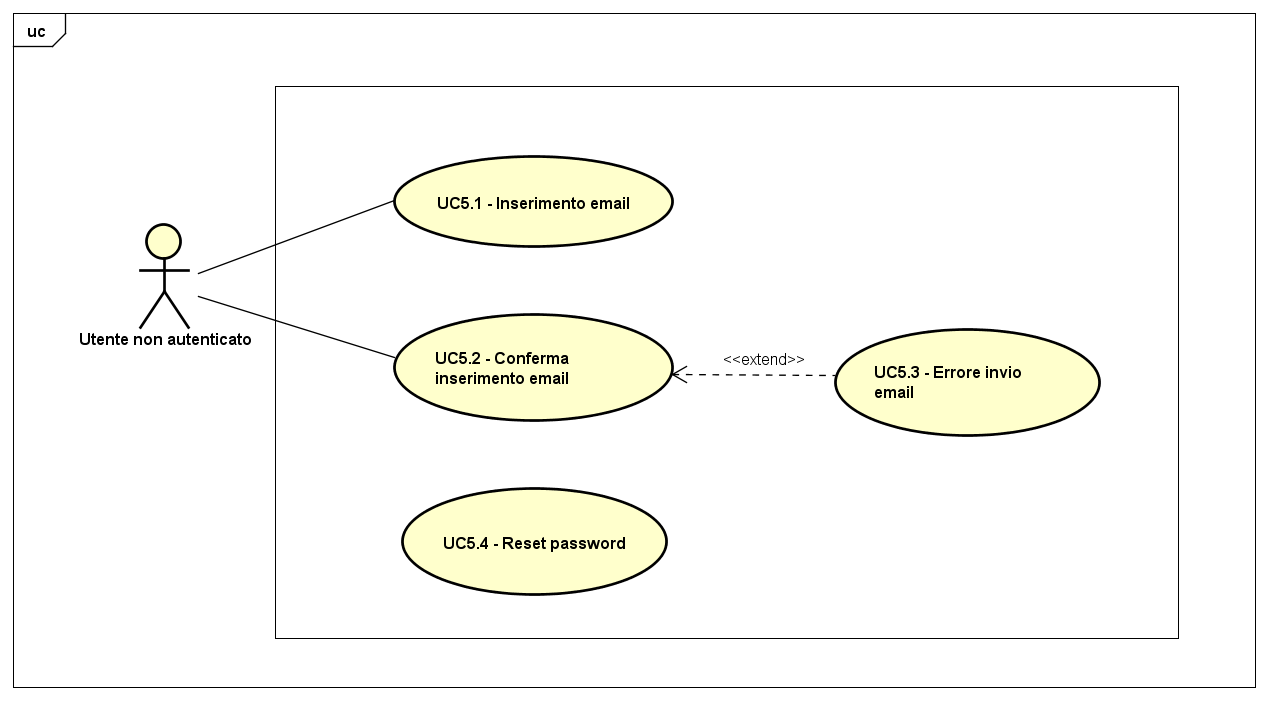
\includegraphics[scale=0.45]{UML/UC5.png}
	\caption{UC5: Recupero password}
\end{figure}

\begin{longtable}{ l | p{11cm}}
	\hline
	\rowcolor{Gray}
	 \multicolumn{2}{c}{UC5 - Recupero password} \\
	 \hline
	\textbf{Attori} & Utente non autenticato \\
	\textbf{Descrizione} & L'attore recupera la password del proprio account API Market tramite l'invio di una email \\
	\textbf{Pre-Condizioni} & L'attore ha scelto di recuperare la password del proprio account API Market \\
	\textbf{Post-Condizioni} & L'attore ha ricevuto nella propria casella email un link per resettare la password del proprio account API Market, oppure la procedura è fallita \\
	\textbf{Scenario Principale} & 
	\begin{enumerate*}[label=(\arabic*.),itemjoin={\newline}]
		\item L'attore può inserire la propria email (UC5.1)
		\item L'attore può confermare l'indirizzo email inserito, al quale l'applicazione web invierà un link per resettare la password (UC5.2)
	\end{enumerate*}\\
	\textbf{Scenari Alternativi} & 
	\begin{enumerate*}[label=(\arabic*.),itemjoin={\newline}]
		\item L'attore, se ha inserito un'email non valida o inesistente, può visualizzare un messaggio d'errore e l'email di reset password non viene inviata (UC5.3)
		\item L'attore, se ha richiesto il recupero della password ed ha aperto il link per poterla resettare, può effettuare il reset password in una apposita schermata (UC5.4)
	\end{enumerate*}\\
\end{longtable}
\subsubsection{Caso d'uso UC5.1: Inserimento email}
\label{UC5_1}

\begin{minipage}{\linewidth}
\begin{longtable}{ l | p{11cm}}
	\hline
	\rowcolor{Gray}
	 \multicolumn{2}{c}{UC5.1 - Inserimento email} \\
	 \hline
	\textbf{Attori} & Utente non autenticato \\
	\textbf{Descrizione} & L'attore inserisce la sua email  \\
	\textbf{Pre-Condizioni} & L'attore ha dimenticato la password e l'applicazione web mostra la schermata di recupero password\\
	\textbf{Post-Condizioni} & L'attore ha inserito l'email relativa all'account che desidera recuperare\\
	\textbf{Scenario Principale} & \begin{enumerate*}[label=(\arabic*.),itemjoin={\newline}]
		\item L'attore può inserire la propria email (UC5.1)
	\end{enumerate*}\\
\end{longtable}
\end{minipage}
\subsubsection{Caso d'uso UC5.2: Conferma inserimento email}
\label{UC5_2}

\begin{minipage}{\linewidth}
\begin{longtable}{ l | p{11cm}}
	\hline
	\rowcolor{Gray}
	 \multicolumn{2}{c}{UC5.2 - Conferma inserimento email} \\
	 \hline
	\textbf{Attori} & Utente non autenticato \\
	\textbf{Descrizione} & L'attore conferma l'inserimento del proprio indirizzo email tramite un apposito pulsante \\
	\textbf{Pre-Condizioni} & L'attore ha inserito l'email dell'account che intende recuperare\\
	\textbf{Post-Condizioni} & L'attore ha compilato il campo email, relativo all'account che desidera recuperare\\
	\textbf{Scenario Principale} & \begin{enumerate*}[label=(\arabic*.),itemjoin={\newline}]
		\item L'attore può confermare i dati immessi, visualizzando un messaggio di successo e ricevendo tramite email la procedura di recupero password (UC5.4) e viene reindirizzato alla schermata principale (UC1)
	\end{enumerate*}\\
	\textbf{Scenari Alternativi} & 
	\begin{enumerate*}[label=(\arabic*.),itemjoin={\newline}]
		\item L'attore ha inserito un email non valida o inesistente, e visualizza un messaggio d'errore (UC5.3)
	\end{enumerate*}\\
\end{longtable}
\end{minipage}
\subsubsection{Caso d'uso UC5.3: Errore invio email}
\label{UC5_3}

\begin{minipage}{\linewidth}
\begin{longtable}{ l | p{11cm}}
	\hline
	\rowcolor{Gray}
	 \multicolumn{2}{c}{UC5.3 - Errore invio email} \\
	 \hline
	\textbf{Attori} & Utente non autenticato \\
	\textbf{Descrizione} & L'attore riceve un messaggio di errore dovuto all'inserimento di un'email non valida o inesistente \\
	\textbf{Pre-Condizioni} & L'attore ha dimenticato la password e ha inserito l'email per poterla recuperare \\
	\textbf{Post-Condizioni} & L'attore riceve un messaggio di errore e può eventualmente ripetere la procedura di recupero password \\
	\textbf{Scenario Principale} & \begin{enumerate*}[label=(\arabic*.),itemjoin={\newline}]
		\item L'attore visualizza un messaggio d'errore per aver lasciato il campo vuoto o per aver inserito un indirizzo inesistente. Può ripetere la procedura (UC5)
	\end{enumerate*}\\
\end{longtable}
\end{minipage}

\newpage
\subsection{Caso d'uso UC6: Ricerca API}
\label{UC6}
\begin{figure}[ht]
	\centering
	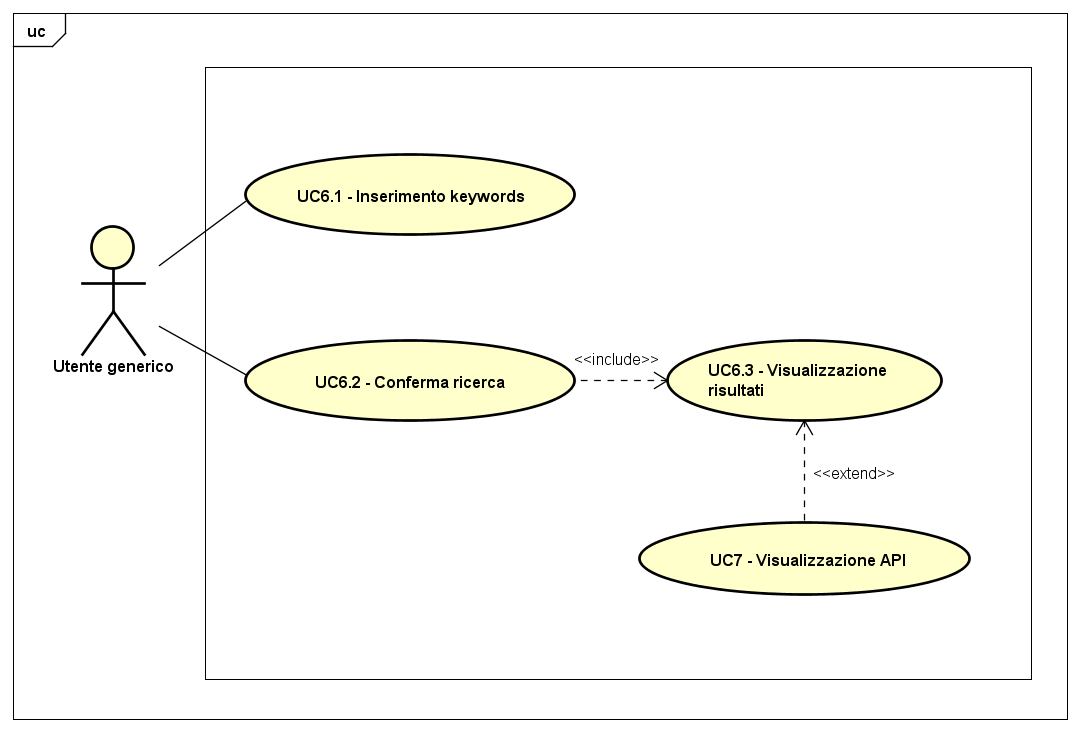
\includegraphics[scale=0.45]{UML/UC6.png}
	\caption{UC6: Ricerca API}
\end{figure}

\begin{longtable}{ l | p{11cm}}
	\hline
	\rowcolor{Gray}
	 \multicolumn{2}{c}{UC6 - Ricerca API} \\
	 \hline
	\textbf{Attori} & Utente generico \\
	\textbf{Descrizione} & L'attore inserisce le keywords per la ricerca di API \\
	\textbf{Pre-Condizioni} & L'attore ha scelto di effettuare una ricerca di API \\
	\textbf{Post-Condizioni} & L'attore ha effettuato la ricerca di API ed ha visualizzato la lista dei risultati \\
	\textbf{Scenario Principale} & 
	\begin{enumerate*}[label=(\arabic*.),itemjoin={\newline}]
		\item L'attore può inserire la stringa di ricerca desiderata (UC6.1)
		\item L'attore può confermare i dati inseriti (UC6.2) e visualizzare i risultati forniti dall'applicazione web (UC6.3)
	\end{enumerate*}\\
\end{longtable}

\subsubsection{Caso d'uso UC6.1: Inserimento keywords}
\label{UC6_1}

\begin{minipage}{\linewidth}
\begin{tabular}{ l | p{11cm}}
	\hline
	\rowcolor{Gray}
	 \multicolumn{2}{c}{UC6.1 - Inserimento keywords} \\
	 \hline
	\textbf{Attori} & Utente generico \\
	\textbf{Descrizione} & L'attore effettua una ricerca delle API inserendo nella barra di ricerca una stringa contenente le keywords desiderate \\
	\textbf{Pre-Condizioni} & L'attore ha scelto di effettuare una ricerca di API \\
	\textbf{Post-Condizioni} & L'attore ha inserito nella barra di ricerca una stringa contenente le keywords desiderate \\
	\textbf{Scenario Principale} & 
	\begin{enumerate*}[label=(\arabic*.),itemjoin={\newline}]
		\item L'attore può inserire nella barra di ricerca una stringa con tenente le keywords desiderate: esse verranno ricercate sul nome dell'API, sul nome dell'autore e su eventuali tag
	\end{enumerate*}\\
\end{tabular}
\end{minipage}

\subsubsection{Caso d'uso UC6.2: Conferma ricerca}
\label{UC6_2}

\begin{minipage}{\linewidth}
	\begin{tabular}{ l | p{11cm}}
		\hline
		\rowcolor{Gray}
		\multicolumn{2}{c}{UC6.2 - Conferma ricerca} \\
		\hline
		\textbf{Attori} & Utente generico \\
		\textbf{Descrizione} & L'attore conferma la stringa di ricerca inserita per poter visualizzare i risultati \\
		\textbf{Pre-Condizioni} & L'attore ha inserito una stringa di ricerca \\
		\textbf{Post-Condizioni} & L'attore ha confermato una stringa di ricerca \\
		\textbf{Scenario Principale} & 
		\begin{enumerate*}[label=(\arabic*.),itemjoin={\newline}]
			\item L'attore può confermare una stringa di ricerca, visualizzando la lista dei risultati (UC6.3)
		\end{enumerate*}\\
	\end{tabular}
\end{minipage}

\newpage
\subsubsection{Caso d'uso UC6.3: Visualizzazione lista risultati}
\label{UC6_3}
\begin{figure}[ht]
	\centering
	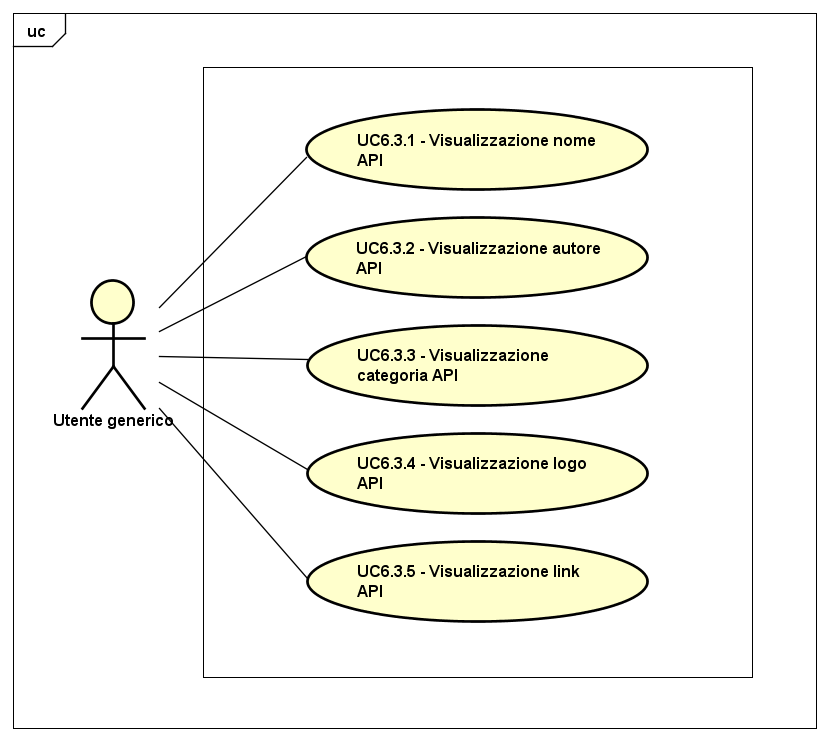
\includegraphics[scale=0.45]{UML/UC6_3.png}
	\caption{UC6.3: Visualizzazione lista risultati}
\end{figure}

\begin{minipage}{\linewidth}
	\begin{tabular}{ l | p{11cm}}
		\hline
		\rowcolor{Gray}
		\multicolumn{2}{c}{UC6.3 - Visualizzazione lista risultati} \\
		\hline
		\textbf{Attori} & Utente generico \\
		\textbf{Descrizione} & L'attore visualizza le API che corrispondono alle keywords della ricerca effettuata \\
		\textbf{Pre-Condizioni} & L'attore ha confermato la ricerca API \\
		\textbf{Post-Condizioni} & L'attore ha visualizzato le API che corrispondono alle keywords della ricerca effettuata \\
		\textbf{Scenario Principale} & 
		\begin{enumerate*}[label=(\arabic*.),itemjoin={\newline}]
			\item L'attore può visualizzare il nome delle API che corrispondono alle keywords della ricerca effettuata (UC6.3.1)
			\
		\end{enumerate*}\\
	\end{tabular}
\end{minipage}

\paragraph{Caso d'uso UC6.3.1: Visualizzazione nome API}
\label{UC6_3_1}

\begin{minipage}{\linewidth}
	\begin{tabular}{ l | p{11cm}}
		\hline
		\rowcolor{Gray}
		\multicolumn{2}{c}{UC6.3.1 - Visualizzazione nome API} \\
		\hline
		\textbf{Attori} & Utente generico \\
		\textbf{Descrizione} & L'attore visualizza nella lista il nome dell'API che corrisponde alle keywords della ricerca effettuata \\
		\textbf{Pre-Condizioni} & L'attore ha confermato la ricerca API \\
		\textbf{Post-Condizioni} & L'attore ha visualizzato nella lista il nome dell'API che corrisponde alle keywords della ricerca effettuata \\
		\textbf{Scenario Principale} & 
		\begin{enumerate*}[label=(\arabic*.),itemjoin={\newline}]
			\item L'attore può visualizzare nella lista il nome dell'API che corrisponde alle keywords della ricerca effettuata
		\end{enumerate*}\\
	\end{tabular}
\end{minipage}

\paragraph{Caso d'uso UC6.3.2: Visualizzazione autore API}
\label{UC6_3_2}

\begin{minipage}{\linewidth}
	\begin{tabular}{ l | p{11cm}}
		\hline
		\rowcolor{Gray}
		\multicolumn{2}{c}{UC6.3.2 - Visualizzazione autore API} \\
		\hline
		\textbf{Attori} & Utente generico \\
		\textbf{Descrizione} & L'attore visualizza nella lista il nome dell'autore dell'API che corrisponde alle keywords della ricerca effettuata \\
		\textbf{Pre-Condizioni} & L'attore ha confermato la ricerca API \\
		\textbf{Post-Condizioni} & L'attore ha visualizzato nella lista il nome dell'autore dell'API che corrisponde alle keywords della ricerca effettuata \\
		\textbf{Scenario Principale} & 
		\begin{enumerate*}[label=(\arabic*.),itemjoin={\newline}]
			\item L'attore può visualizzare nella lista il nome dell'autore dell'API che corrisponde alle keywords della ricerca effettuata
		\end{enumerate*}\\
	\end{tabular}
\end{minipage}

\paragraph{Caso d'uso UC6.3.3: Visualizzazione categoria API}
\label{UC6_3_3}

\begin{minipage}{\linewidth}
	\begin{tabular}{ l | p{11cm}}
		\hline
		\rowcolor{Gray}
		\multicolumn{2}{c}{UC6.3.3 - Visualizzazione categoria API} \\
		\hline
		\textbf{Attori} & Utente generico \\
		\textbf{Descrizione} & L'attore visualizza nella lista la categoria dell'API che corrisponde alle keywords della ricerca effettuata \\
		\textbf{Pre-Condizioni} & L'attore ha confermato la ricerca API \\
		\textbf{Post-Condizioni} & L'attore ha visualizzato nella lista la categoria dell'API che corrisponde alle keywords della ricerca effettuata \\
		\textbf{Scenario Principale} & 
		\begin{enumerate*}[label=(\arabic*.),itemjoin={\newline}]
			\item L'attore può visualizzare nella lista la categoria dell'API che corrisponde alle keywords della ricerca effettuata
		\end{enumerate*}\\
	\end{tabular}
\end{minipage}

\paragraph{Caso d'uso UC6.3.4: Visualizzazione logo API}
\label{UC6_3_4}

\begin{minipage}{\linewidth}
	\begin{tabular}{ l | p{11cm}}
		\hline
		\rowcolor{Gray}
		\multicolumn{2}{c}{UC6.3.4 - Visualizzazione logo API} \\
		\hline
		\textbf{Attori} & Utente generico \\
		\textbf{Descrizione} & L'attore visualizza nella lista il logo dell'API che corrisponde alle keywords della ricerca effettuata \\
		\textbf{Pre-Condizioni} & L'attore ha confermato la ricerca API \\
		\textbf{Post-Condizioni} & L'attore ha visualizzato nella lista il logo dell'API che corrisponde alle keywords della ricerca effettuata \\
		\textbf{Scenario Principale} & 
		\begin{enumerate*}[label=(\arabic*.),itemjoin={\newline}]
			\item L'attore può visualizzare nella lista il logo dell'API che corrisponde alle keywords della ricerca effettuata
		\end{enumerate*}\\
	\end{tabular}
\end{minipage}

\paragraph{Caso d'uso UC6.3.5: Visualizzazione link API}
\label{UC6_3_5}

\begin{minipage}{\linewidth}
	\begin{tabular}{ l | p{11cm}}
		\hline
		\rowcolor{Gray}
		\multicolumn{2}{c}{UC6.3.5 - Visualizzazione link API} \\
		\hline
		\textbf{Attori} & Utente generico \\
		\textbf{Descrizione} & L'attore visualizza nella lista il link alla visualizzazione dell'API che corrisponde alle keywords della ricerca effettuata \\
		\textbf{Pre-Condizioni} & L'attore ha confermato la ricerca API \\
		\textbf{Post-Condizioni} & L'attore ha visualizzato nella lista il link alla visualizzazione dell'API che corrisponde alle keywords della ricerca effettuata \\
		\textbf{Scenario Principale} & 
		\begin{enumerate*}[label=(\arabic*.),itemjoin={\newline}]
			\item L'attore può visualizzare nella lista il link alla visualizzazione dell'API che corrisponde alle keywords della ricerca effettuata, che lo reindirizzerà ad UC7 per l'API in questione
		\end{enumerate*}\\
	\end{tabular}
\end{minipage}
\subsubsection{Caso d'uso UC6.1:  Inserimento Nome API}
\label{UC6_1}

\begin{tabular}{ l | p{11cm}}
	\hline
	\rowcolor{Gray}
	 \multicolumn{2}{c}{UC6.1 - Inserimento Nome API} \\
	 \hline
	\textbf{Attori} & Utente Non Autenticato, Utente Autenticato \\
	\textbf{Descrizione} & Gli utenti possono effettuare una ricerca delle API usandone il nome\\
	\textbf{Pre-Condizioni} & L'utente ha scelto fare una ricerca di API\\
	\textbf{Post-Condizioni} & L'utente ha inserito il nome dell'API nella barra di ricerca \\
	\textbf{Scenario Principale} & 
	\begin{enumerate*}[label=(\arabic*.),itemjoin={\newline}]
		\item L'utente puo' inserire il Nome dell API nella barra di ricerca (UC6.1)
	\end{enumerate*}\\
\end{tabular}
\subsubsection{Caso d'uso UC6.2: Conferma ricerca}
\label{UC6_2}

\begin{minipage}{\linewidth}
	\begin{tabular}{ l | p{11cm}}
		\hline
		\rowcolor{Gray}
		\multicolumn{2}{c}{UC6.2 - Conferma ricerca} \\
		\hline
		\textbf{Attori} & Utente non autenticato, Utente autenticato \\
		\textbf{Descrizione} & L'attore conferma la stringa di ricerca inserita per poter visualizzare i risultati\\
		\textbf{Pre-Condizioni} & L'attore ha inserito una stringa di ricerca\\
		\textbf{Post-Condizioni} & L'attore ha confermato una stringa per la ricerca \\
		\textbf{Scenario Principale} & 
		\begin{enumerate*}[label=(\arabic*.),itemjoin={\newline}]
			\item L'attore può confermare una stringa per la ricerca
		\end{enumerate*}\\
	\end{tabular}
\end{minipage}
\subsubsection{Caso d'uso UC6.3: Visualizza risultati}
\label{UC6_3}

\begin{minipage}{\linewidth}
	\begin{tabular}{ l | p{11cm}}
		\hline
		\rowcolor{Gray}
		\multicolumn{2}{c}{UC6.3 - Visualizza risultati} \\
		\hline
		\textbf{Attori} & Utente non autenticato, Utente autenticato \\
		\textbf{Descrizione} & L'attore visualizza i risultati prodotti dalla piattaforma\\
		\textbf{Pre-Condizioni} & L'attore ha confermato la ricerca\\
		\textbf{Post-Condizioni} & L'attore visualizza i risultati di ricerca prodotti \\
		\textbf{Scenario Principale} & 
		\begin{enumerate*}[label=(\arabic*.),itemjoin={\newline}]
			\item L'attore può visualizzare i risultati della ricerca, che possono essere anche vuoti nel caso di stringhe non consone. L'utente può accedere alla schermata delle singole API (UC7)
		\end{enumerate*}\\
	\end{tabular}
\end{minipage}
\newpage
\subsection{Caso d'uso UC7 - Visualizzazione API}
\label{UC7}
\begin{figure}[ht]
	\centering
	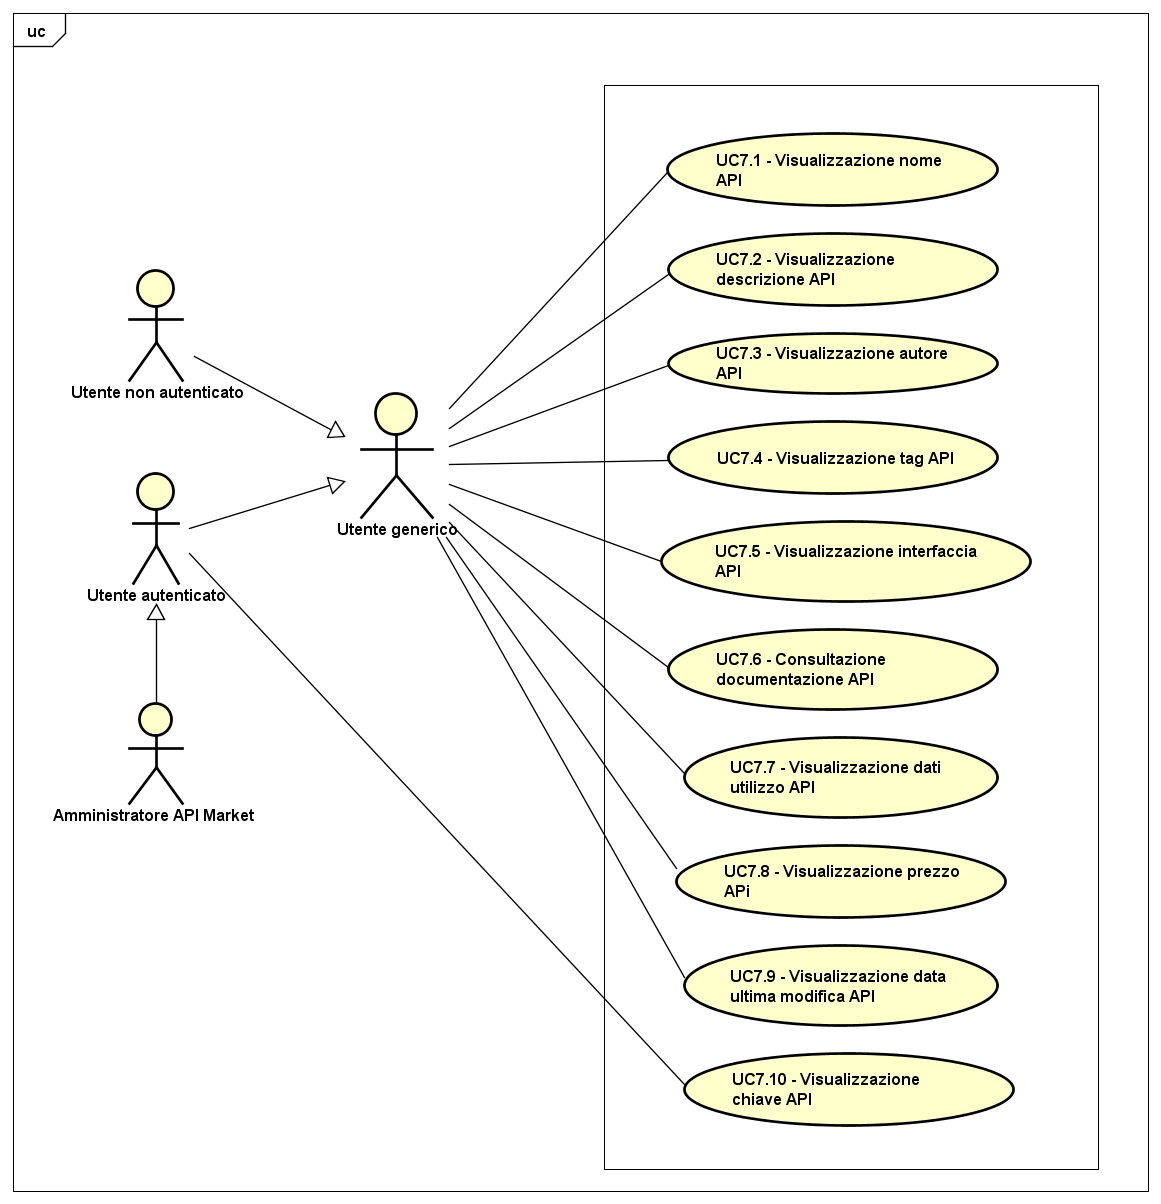
\includegraphics[scale=0.45]{UML/UC7.png}
	\caption{UC7: Visualizzazione API}
\end{figure}

\begin{longtable}{ l | p{11cm}}
	\hline
	\rowcolor{Gray}
	\multicolumn{2}{c}{UC7 - Visualizzazione API}\\
	\hline
	
	 \textbf{Attori} & Utente non autenticato, Utente autenticato  \\
	\textbf{Descrizione} & L'attore può visualizzare i dati relativi a un API che ha selezionato tramite la homepage o i risultati di una ricerca  \\
	\textbf{Pre-Condizioni} & L'attore ha selezionato un prodotto per la consultazione \\
	\textbf{Post-Condizioni} & L'attore visualizza la pagina relativa all'API selezionata\\
	\textbf{Scenario Principale} & 
	\begin{enumerate*}[label=(\arabic*.),itemjoin={\newline}]
		\item L'attore visualizza il nome dell'API (UC7.1)
		\item L'attore visualizza la descrizione dell'API (UC7.2)
		\item L'attore visualizza l'autore dell'API (UC7.3)
		\item L'attore può visualizzare l'interfaccia dell'API (UC7.4)
		\item L'attore può consultare la documentazione fornita dall'utente (UC7.5)
		\item L'utente può visualizzare i dati di utilizzo dell'API  (UC7.6)
	\end{enumerate*}\\
\end{longtable}

\newpage
\subsection{Caso d'uso UC8: Visualizzazione API acquistate}
\label{UC8}
\begin{figure}[ht]
	\centering
	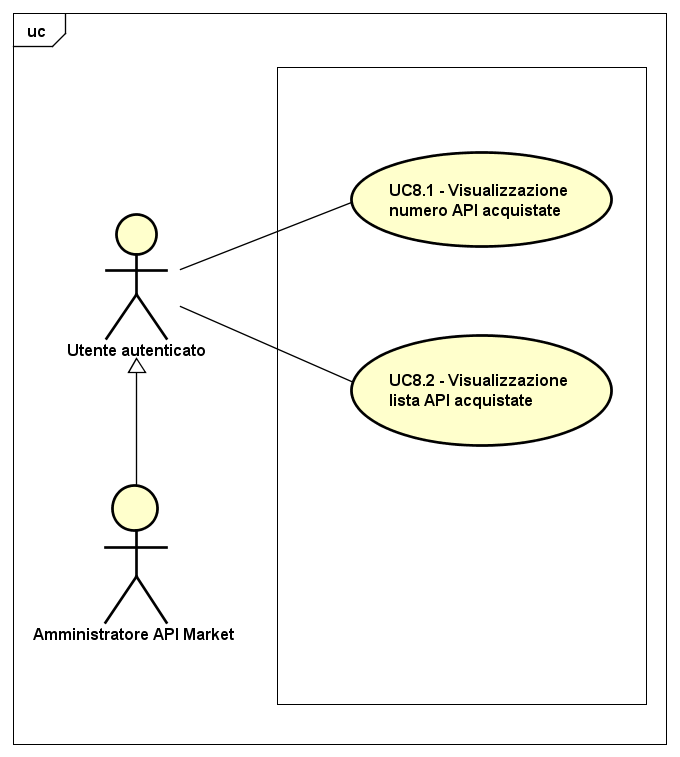
\includegraphics[scale=0.45]{UML/UC8.png}
	\caption{UC8: Visualizzazione API acquistate}
\end{figure}

\begin{longtable}{ l | p{11cm}}
	\hline
	\rowcolor{Gray}
	\multicolumn{2}{c}{UC8 - Visualizzazione API acquistate}\\
	\hline
	 \textbf{Attori} & Utente autenticato, Amministratore API Market \\
	\textbf{Descrizione} & L'attore visualizza le API da lui acquistate \\
	\textbf{Pre-Condizioni} & L'attore si trova nella schermata relativa alle API da lui acquistate \\
	\textbf{Post-Condizioni} & L'attore ha visualizzato le API da lui acquistate \\
	\textbf{Scenario Principale} & 
	\begin{enumerate*}[label=(\arabic*.),itemjoin={\newline}]
		\item L'attore può visualizzare il numero delle API acquistate e attive (UC8.1)
		\item L'attore può visualizzare la lista delle API acquistate e attive (UC8.2)
	\end{enumerate*}\\
\end{longtable}

\subsubsection{Caso d'uso UC8.1: Visualizzazione numero API acquistate}
\label{UC8_1}

\begin{minipage}{\linewidth}
	\begin{tabular}{ l | p{11cm}}
		\hline
		\rowcolor{Gray}
		\multicolumn{2}{c}{UC8.1 - Visualizzazione numero API acquistate} \\
		\hline
		\textbf{Attori} & Utente autenticato, Amministratore API Market \\
		\textbf{Descrizione} & L'attore visualizza il numero di API da lui acquistate \\
		\textbf{Pre-Condizioni} & L'attore si trova nella schermata relativa alle API da lui acquistate \\
		\textbf{Post-Condizioni} & L'attore ha visualizzato il numero delle API da lui acquistate \\
		\textbf{Scenario Principale} & 
		\begin{enumerate*}[label=(\arabic*.),itemjoin={\newline}]
			\item L'attore può visualizzare il numero di API acquistate
		\end{enumerate*}\\
	\end{tabular}
\end{minipage}

\newpage
\subsubsection{Caso d'uso UC8.2: Visualizzazione lista API acquistate}
\label{UC8_2}
\begin{figure}[ht]
	\centering
	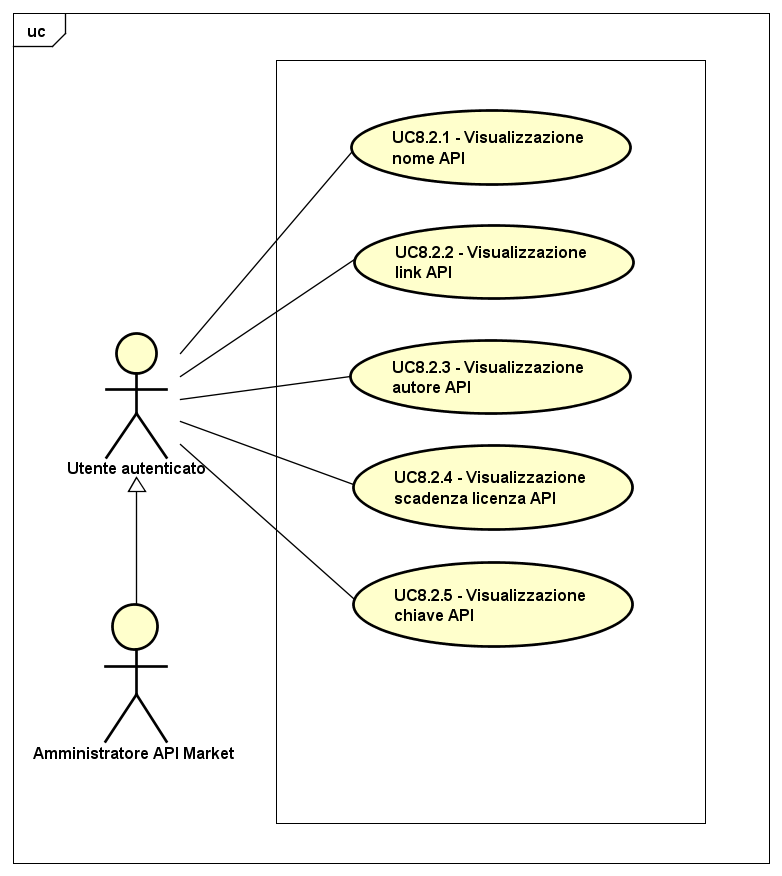
\includegraphics[scale=0.45]{UML/UC8_2.png}
	\caption{UC8.2: Visualizzazione lista API acquistate}
\end{figure}

\begin{minipage}{\linewidth}
	\begin{tabular}{ l | p{11cm}}
		\hline
		\rowcolor{Gray}
		\multicolumn{2}{c}{UC8.2 - Visualizzazione lista API acquistate} \\
		\hline
		\textbf{Attori} & Utente autenticato, Amministratore API Market \\
		\textbf{Descrizione} & L'attore visualizza la lista delle API da lui acquistate \\
		\textbf{Pre-Condizioni} & L'attore si trova nella schermata relativa alle API da lui acquistate \\
		\textbf{Post-Condizioni} & L'attore ha visualizzato la lista delle API da lui acquistate \\
		\textbf{Scenario Principale} & 
		\begin{enumerate*}[label=(\arabic*.),itemjoin={\newline}]
			\item L'attore può visualizzare il nome dell'API (UC8.2.1)
			\item L'attore può visualizzare il link alla pagina di visualizzazione API (UC8.2.2)
			\item L'attore può visualizzare il nome dell'autore dell'API (UC8.2.3)
			\item L'attore può visualizzare la policy divendita dell'API (UC8.2.4)
			\item L'attore può visualizzare il parametro di scadenza, in base al contratto,  della propria licenza per l'API (UC8.2.5)
			\item L'attore può visualizzare gli avvisi riguardo l'API (UC8.2.6)
		\end{enumerate*}\\
	\end{tabular}
\end{minipage}

\paragraph{Caso d'uso UC8.2.1: Visualizzazione nome API}
\label{UC8_2_1}

\begin{minipage}{\linewidth}
	\begin{tabular}{ l | p{11cm}}
		\hline
		\rowcolor{Gray}
		\multicolumn{2}{c}{UC8.2.1 - Visualizzazione nome API} \\
		\hline
		\textbf{Attori} & Utente autenticato, Amministratore API Market \\
		\textbf{Descrizione} & L'attore visualizza nella lista il nome dell'API \\
		\textbf{Pre-Condizioni} & L'attore si trova nella schermata relativa alle API da lui acquistate \\
		\textbf{Post-Condizioni} & L'attore ha visualizzato nella lista il nome dell'API \\
		\textbf{Scenario Principale} & 
		\begin{enumerate*}[label=(\arabic*.),itemjoin={\newline}]
			\item L'attore può visualizzare nella lista il nome dell'API
		\end{enumerate*}\\
	\end{tabular}
\end{minipage}

\paragraph{Caso d'uso UC8.2.2: Visualizzazione link API}
\label{UC8_2_2}

\begin{minipage}{\linewidth}
	\begin{tabular}{ l | p{11cm}}
		\hline
		\rowcolor{Gray}
		\multicolumn{2}{c}{UC8.2.2 - Visualizzazione link API} \\
		\hline
		\textbf{Attori} & Utente autenticato, Amministratore API Market \\
		\textbf{Descrizione} & L'attore visualizza nella lista il link alla visualizzazione dell'API \\
		\textbf{Pre-Condizioni} & L'attore si trova nella schermata di visualizzazione delle API acquistate \\
		\textbf{Post-Condizioni} & L'attore ha visualizzato nella lista il link alla visualizzazione dell'API \\
		\textbf{Scenario Principale} & 
		\begin{enumerate*}[label=(\arabic*.),itemjoin={\newline}]
			\item L'attore può visualizzare nella lista il link alla visualizzazione dell'API, che lo reindirizzerà ad UC7 per l'API in questione
		\end{enumerate*}\\
	\end{tabular}
\end{minipage}

\paragraph{Caso d'uso UC8.2.3: Visualizzazione nome autore API}
\label{UC8_2_3}

\begin{minipage}{\linewidth}
	\begin{tabular}{ l | p{11cm}}
		\hline
		\rowcolor{Gray}
		\multicolumn{2}{c}{UC8.2.3 - Visualizzazione nome autore API} \\
		\hline
		\textbf{Attori} & Utente autenticato, Amministratore API Market \\
		\textbf{Descrizione} & L'attore visualizza nella lista il nome dell'autore dell'API \\
		\textbf{Pre-Condizioni} & L'attore si trova nella schermata relativa alle API da lui acquistate \\
		\textbf{Post-Condizioni} & L'attore ha visualizzato nella lista il nome dell'autore dell'API \\
		\textbf{Scenario Principale} & 
		\begin{enumerate*}[label=(\arabic*.),itemjoin={\newline}]
			\item L'attore può visualizzare nella lista il nome dell'autore dell'API
		\end{enumerate*}\\
	\end{tabular}
\end{minipage}

\paragraph{Caso d'uso UC8.2.4: Visualizzazione policy vendita API}
\label{UC8_2_4}

\begin{minipage}{\linewidth}
	\begin{tabular}{ l | p{11cm}}
		\hline
		\rowcolor{Gray}
		\multicolumn{2}{c}{UC8.2.4 - Visualizzazione policy vendita API} \\
		\hline
		\textbf{Attori} & Utente autenticato, Amministratore API Market \\
		\textbf{Descrizione} & L'attore visualizza nella lista la policy di vendita dell'API \\
		\textbf{Pre-Condizioni} & L'attore si trova nella schermata relativa alle API da lui acquistate \\
		\textbf{Post-Condizioni} & L'attore ha visualizzato nella lista la policy di vendita dell'API \\
		\textbf{Scenario Principale} & 
		\begin{enumerate*}[label=(\arabic*.),itemjoin={\newline}]
			\item L'attore può visualizzare nella lista la policy di vendita dell'API
		\end{enumerate*}\\
	\end{tabular}
\end{minipage}

\paragraph{Caso d'uso UC8.2.5: Visualizzazione scadenza licenza}
\label{UC8_2_5}

\begin{minipage}{\linewidth}
	\begin{tabular}{ l | p{11cm}}
		\hline
		\rowcolor{Gray}
		\multicolumn{2}{c}{UC8.2.3 - Visualizzazione scadenza licenza} \\
		\hline
		\textbf{Attori} & Utente autenticato, Amministratore API Market \\
		\textbf{Descrizione} & L'attore visualizza nella lista la data di scadenza della propria licenza per l'API \\
		\textbf{Pre-Condizioni} & L'attore si trova nella schermata relativa alle API da lui acquistate \\
		\textbf{Post-Condizioni} & L'attore ha visualizzato nella lista il parametro di scadenza dell'API \\
		\textbf{Scenario Principale} & 
		\begin{enumerate*}[label=(\arabic*.),itemjoin={\newline}]
			\item L'attore può visualizzare nella lista il parametro di scadenza della propria licenza per l'API
		\end{enumerate*}\\
	\end{tabular}
\end{minipage}

\paragraph{Caso d'uso UC8.2.6: Avvisi API}
\label{UC8_2_6}

\begin{minipage}{\linewidth}
	\begin{tabular}{ l | p{11cm}}
		\hline
		\rowcolor{Gray}
		\multicolumn{2}{c}{UC8.2.6 - Avvisi API} \\
		\hline
		\textbf{Attori} & Utente autenticato, Amministratore API Market \\
		\textbf{Descrizione} & L'attore visualizza nella lista gli avvisi riguardanti l'API \\
		\textbf{Pre-Condizioni} & L'attore si trova nella schermata relativa alle API da lui acquistate \\
		\textbf{Post-Condizioni} & L'attore ha visualizzato nella lista gli avvisi riguardanti l'API \\
		\textbf{Scenario Principale} & 
		\begin{enumerate*}[label=(\arabic*.),itemjoin={\newline}]
			\item L'attore può visualizzare nella lista gli avvisi riguardanti l'API (E.g: cancellazione, manutenzione)
		\end{enumerate*}\\
	\end{tabular}
\end{minipage}
\newpage
\subsection{Caso d'uso UC9: Acquisto API}
\label{UC9}
\begin{figure}[ht]
	\centering
	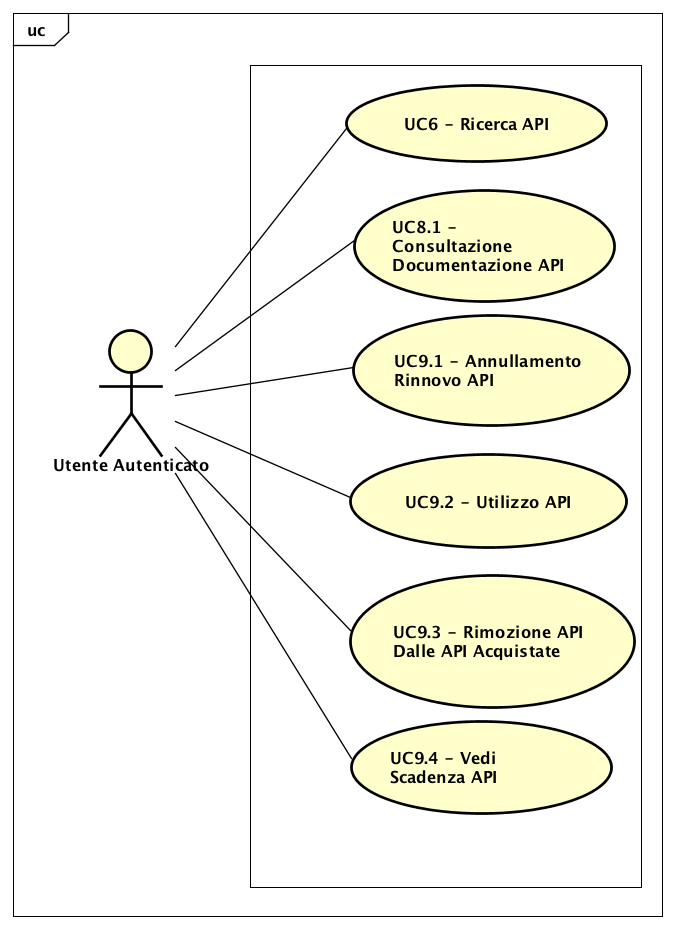
\includegraphics[scale=0.45]{UML/UC9.png}
	\caption{UC9: Acquisto API}
\end{figure}

\begin{longtable}{ l | p{11cm}}
	\hline
	\rowcolor{Gray}
	\multicolumn{2}{c}{UC9 - Acquisto API}\\
	\hline
	\textbf{Attori} & Utente autenticato, Amministratore API Market \\
	\textbf{Descrizione} & L'attore può effettuare l'acquisto dell'API selezionata tramite i crediti da lui posseduti \\
	\textbf{Pre-Condizioni} & L'attore ha selezionato una API e si trova nella relativa schermata di acquisto \\
	\textbf{Post-Condizioni} & L'attore ha acquistato l'API selezionata \\
	\textbf{Scenario Principale} & 
	\begin{enumerate*}[label=(\arabic*.),itemjoin={\newline}]
		\item L'attore può visualizzare il nome dell'API (UC9.1)
		\item L'attore può visualizzare l'autore dell'API (UC9.2)
		\item L'attore può scegliere la licenza API desiderata (UC9.3)
		\item L'attore può visualizzare il prezzo dell'API selezionata (UC9.4)
		\item L'attore può visualizzare il saldo disponibile nel suo conto virtuale (UC12.2.1)
		\item L'attore può ricaricare il proprio conto virtuale (UC12.2.2)
		\item L'attore può visualizzare il saldo preventivato in seguito all'acquisto della licenza selezionata (UC9.5)
		\item L'attore può confermare l'acquisto (UC9.6), venendo reindirizzato ad una schermata di riepilogo (UC9.7)
	\end{enumerate*}\\
	\textbf{Scenari Alternativi} & 
	\begin{enumerate*}[label=(\arabic*.),itemjoin={\newline}]
		\item L'attore può visualizzare un messaggio di errore e la transazione non avviene (UC9.8)
	\end{enumerate*}\\
\end{longtable}

\subsubsection{Caso d'uso UC9.1: Visualizzazione nome API}
\label{UC9_1}

\begin{minipage}{\linewidth}
	\begin{tabular}{ l | p{11cm}}
		\hline
		\rowcolor{Gray}
		\multicolumn{2}{c}{UC9.1 - Visualizzazione nome API} \\
		\hline
		\textbf{Attori} & Utente autenticato, Amministratore API Market \\
		\textbf{Descrizione} & L'attore visualizza il nome dell'API \\
		\textbf{Pre-Condizioni} & L'attore si trova nella schermata di acquisto dell'API \\
		\textbf{Post-Condizioni} & L'attore ha visualizzato il nome dell'API \\
		\textbf{Scenario Principale} & 
		\begin{enumerate*}[label=(\arabic*.),itemjoin={\newline}]
			\item L'attore può visualizzare il nome dell'API
		\end{enumerate*}\\
	\end{tabular}
\end{minipage}

\subsubsection{Caso d'uso UC9.2: Visualizzazione nome API}
\label{UC9_2}

\begin{minipage}{\linewidth}
	\begin{tabular}{ l | p{11cm}}
		\hline
		\rowcolor{Gray}
		\multicolumn{2}{c}{UC9.2 - Visualizzazione autore API} \\
		\hline
		\textbf{Attori} & Utente autenticato, Amministratore API Market \\
		\textbf{Descrizione} & L'attore visualizza l'autore dell'API \\
		\textbf{Pre-Condizioni} & L'attore si trova nella schermata di acquisto dell'API \\
		\textbf{Post-Condizioni} & L'attore ha visualizzato l'autore dell'API \\
		\textbf{Scenario Principale} & 
		\begin{enumerate*}[label=(\arabic*.),itemjoin={\newline}]
			\item L'attore può visualizzare l'autore dell'API
		\end{enumerate*}\\
	\end{tabular}
\end{minipage}

\newpage
\subsubsection{Caso d'uso UC9.3: Scelta licenza API}
\label{UC9_3}
\begin{figure}[ht]
	\centering
	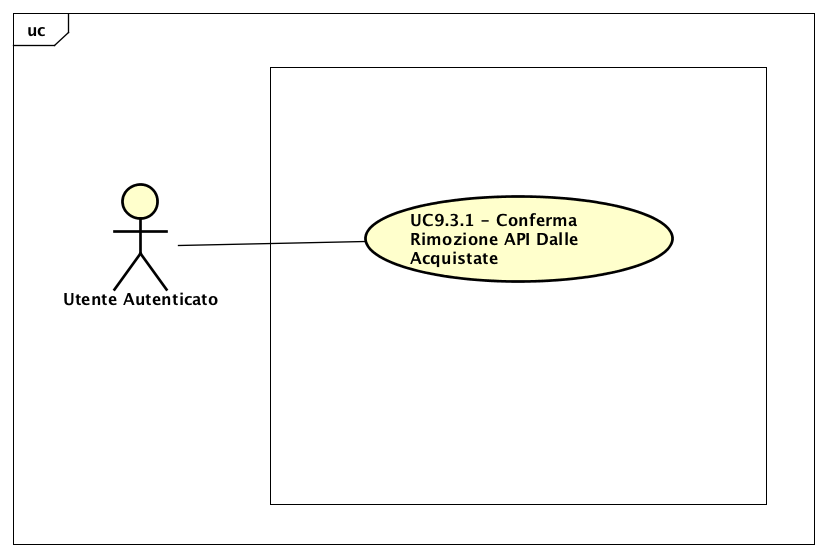
\includegraphics[scale=0.45]{UML/UC9_3.png}
	\caption{UC9.3: Scelta licenza API}
\end{figure}

\begin{minipage}{\linewidth}
	\begin{tabular}{ l | p{11cm}}
		\hline
		\rowcolor{Gray}
		\multicolumn{2}{c}{UC9.1 - Visualizzazione menù licenza} \\
		\hline
		\textbf{Attori} & Utente autenticato, Amministratore API Market \\
		\textbf{Descrizione} & L'attore sceglie tra le licenze quella desiderata, oppure lascia inalterata la scelta di default \\
		\textbf{Pre-Condizioni} & L'attore ha selezionato una API e si trova nella relativa schermata di acquisto \\
		\textbf{Post-Condizioni} & L'attore ha selezionato la licenza desiderata, oppure ha lasciato inalterata la scelta di default \\
		\textbf{Scenario Principale} & 
		\begin{enumerate*}[label=(\arabic*.),itemjoin={\newline}]
			\item L'attore può selezionare la licenza per numero di chiamate, impostata di default (UC9.3.1)
			\item L'attore può selezionare la licenza per tempo di utilizzo (UC9.3.2)
			\item L'attore può selezionare la licenza per traffico (UC9.3.3)
		\end{enumerate*}\\
	\end{tabular}
\end{minipage}

\paragraph{Caso d'uso UC9.3.1: Scelta licenza per numero di chiamate}
\label{UC9_3_1}

\begin{minipage}{\linewidth}
	\begin{tabular}{ l | p{11cm}}
		\hline
		\rowcolor{Gray}
		\multicolumn{2}{c}{UC9.3.1 - Scelta licenza per numero di chiamate} \\
		\hline
		\textbf{Attori} & Utente autenticato, Amministratore API Market \\
		\textbf{Descrizione} & L'attore sceglie la licenza API per numero di chiamate \\
		\textbf{Pre-Condizioni} & L'attore si trova nella schermata di acquisto dell'API \\
		\textbf{Post-Condizioni} & L'attore ha scelto la licenza API per numero di chiamate \\
		\textbf{Scenario Principale} & 
		\begin{enumerate*}[label=(\arabic*.),itemjoin={\newline}]
			\item L'attore può scegliere la licenza API per numero di chiamate
		\end{enumerate*}\\
	\end{tabular}
\end{minipage}

\paragraph{Caso d'uso UC9.3.2: Scelta licenza per tempo di utilizzo}
\label{UC9_3_2}

\begin{minipage}{\linewidth}
	\begin{tabular}{ l | p{11cm}}
		\hline
		\rowcolor{Gray}
		\multicolumn{2}{c}{UC9.3.2 - Scelta licenza per tempo di utilizzo} \\
		\hline
		\textbf{Attori} & Utente autenticato, Amministratore API Market \\
		\textbf{Descrizione} & L'attore sceglie la licenza API per tempo di utilizzo \\
		\textbf{Pre-Condizioni} & L'attore si trova nella schermata di acquisto dell'API \\
		\textbf{Post-Condizioni} & L'attore ha scelto la licenza API per tempo di utilizzo \\
		\textbf{Scenario Principale} & 
		\begin{enumerate*}[label=(\arabic*.),itemjoin={\newline}]
			\item L'attore può scegliere la licenza API per tempo di utilizzo
		\end{enumerate*}\\
	\end{tabular}
\end{minipage}

\paragraph{Caso d'uso UC9.3.3: Scelta licenza per traffico}
\label{UC9_3_3}

\begin{minipage}{\linewidth}
	\begin{tabular}{ l | p{11cm}}
		\hline
		\rowcolor{Gray}
		\multicolumn{2}{c}{UC9.3.3 - Scelta licenza per traffico} \\
		\hline
		\textbf{Attori} & Utente autenticato, Amministratore API Market \\
		\textbf{Descrizione} & L'attore sceglie la licenza API per traffico \\
		\textbf{Pre-Condizioni} & L'attore si trova nella schermata di acquisto dell'API \\
		\textbf{Post-Condizioni} & L'attore ha scelto la licenza API per traffico \\
		\textbf{Scenario Principale} & 
		\begin{enumerate*}[label=(\arabic*.),itemjoin={\newline}]
			\item L'attore può scegliere la licenza API per traffico
		\end{enumerate*}\\
	\end{tabular}
\end{minipage}

\newpage
\subsubsection{Caso d'uso UC9.4: Visualizzazione prezzo API}
\label{UC9_4}
\begin{figure}[ht]
	\centering
	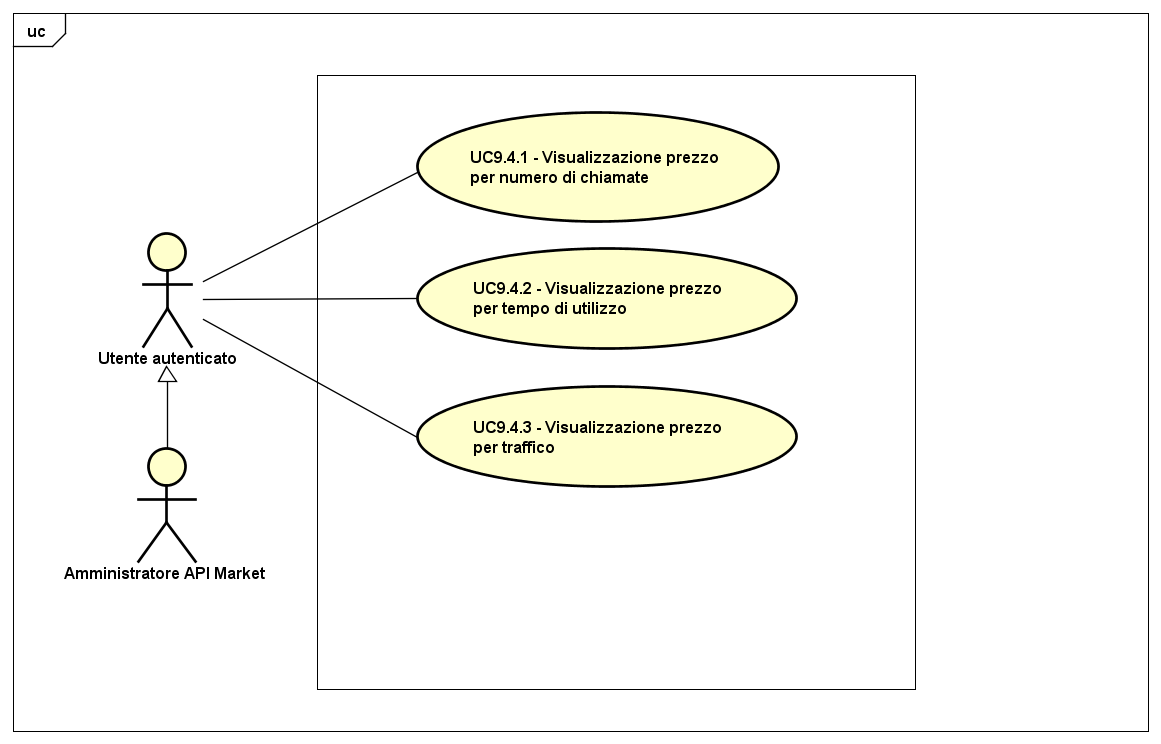
\includegraphics[scale=0.45]{UML/UC9_4.png}
	\caption{UC9.4: Visualizzazione prezzo API}
\end{figure}

\begin{minipage}{\linewidth}
	\begin{tabular}{ l | p{11cm}}
		\hline
		\rowcolor{Gray}
		\multicolumn{2}{c}{UC9.4 - Visualizzazione prezzo API} \\
		\hline
		\textbf{Attori} & Utente autenticato, Amministratore API Market \\
		\textbf{Descrizione} & L'attore visualizza il prezzo dell'API \\
		\textbf{Pre-Condizioni} & L'attore si trova nella schermata di acquisto dell'API \\
		\textbf{Post-Condizioni} & L'attore ha visualizzato il prezzo dell'API \\
		\textbf{Scenario Principale} & 
		\begin{enumerate*}[label=(\arabic*.),itemjoin={\newline}]
			\item L'attore può visualizzare il prezzo dell'API per numero di chiamate (UC9.4.1)
			\item L'attore può visualizzare il prezzo dell'API per tempo di utilizzo (UC9.4.2)
			\item L'attore può visualizzare il prezzo dell'API per traffico (UC9.4.3)
		\end{enumerate*}\\
	\end{tabular}
\end{minipage}

\paragraph{Caso d'uso UC9.4.1: Visualizzazione prezzo per numero di chiamate}
\label{UC9_4_1}

\begin{minipage}{\linewidth}
	\begin{tabular}{ l | p{11cm}}
		\hline
		\rowcolor{Gray}
		\multicolumn{2}{c}{UC9.4.1 - Visualizzazione prezzo per numero di chiamate} \\
		\hline
		\textbf{Attori} & Utente autenticato, Amministratore API Market \\
		\textbf{Descrizione} & L'attore visualizza il prezzo per numero di chiamate dell'API \\
		\textbf{Pre-Condizioni} & L'attore si trova nella schermata di acquisto dell'API \\
		\textbf{Post-Condizioni} & L'attore ha visualizzato il prezzo per numero di chiamate dell'API \\
		\textbf{Scenario Principale} & 
		\begin{enumerate*}[label=(\arabic*.),itemjoin={\newline}]
			\item L'attore può visualizzare il prezzo per numero di chiamate dell'API
		\end{enumerate*}\\
	\end{tabular}
\end{minipage}

\paragraph{Caso d'uso UC9.4.2: Visualizzazione prezzo per tempo di utilizzo}
\label{UC9_4_2}

\begin{minipage}{\linewidth}
	\begin{tabular}{ l | p{11cm}}
		\hline
		\rowcolor{Gray}
		\multicolumn{2}{c}{UC9.4.2 - Visualizzazione prezzo per tempo di utilizzo} \\
		\hline
		\textbf{Attori} & Utente autenticato, Amministratore API Market \\
		\textbf{Descrizione} & L'attore visualizza il prezzo per tempo di utilizzo dell'API \\
		\textbf{Pre-Condizioni} & L'attore si trova nella schermata di acquisto dell'API \\
		\textbf{Post-Condizioni} & L'attore ha visualizzato il prezzo per tempo di utilizzo dell'API \\
		\textbf{Scenario Principale} & 
		\begin{enumerate*}[label=(\arabic*.),itemjoin={\newline}]
			\item L'attore può visualizzare il prezzo per tempo di utilizzo dell'API
		\end{enumerate*}\\
	\end{tabular}
\end{minipage}

\paragraph{Caso d'uso UC9.4.3: Visualizzazione prezzo per traffico}
\label{UC9_4_3}

\begin{minipage}{\linewidth}
	\begin{tabular}{ l | p{11cm}}
		\hline
		\rowcolor{Gray}
		\multicolumn{2}{c}{UC9.4.3 - Visualizzazione prezzo per traffico} \\
		\hline
		\textbf{Attori} & Utente autenticato, Amministratore API Market \\
		\textbf{Descrizione} & L'attore visualizza il prezzo per per traffico dell'API \\
		\textbf{Pre-Condizioni} & L'attore si trova nella schermata di acquisto dell'API \\
		\textbf{Post-Condizioni} & L'attore ha visualizzato il prezzo per per traffico dell'API \\
		\textbf{Scenario Principale} & 
		\begin{enumerate*}[label=(\arabic*.),itemjoin={\newline}]
			\item L'attore può visualizzare il prezzo per per traffico dell'API
		\end{enumerate*}\\
	\end{tabular}
\end{minipage}

\subsubsection{Caso d'uso UC9.5: Visualizzazione previsione saldo finale}
\label{UC9_5}

\begin{minipage}{\linewidth}
	\begin{tabular}{ l | p{11cm}}
		\hline
		\rowcolor{Gray}
		\multicolumn{2}{c}{UC9.5 - Visualizzazione previsione saldo finale} \\
		\hline
		\textbf{Attori} & Utente autenticato, Amministratore API Market \\
		\textbf{Descrizione} & L'attore visualizza una previsione del proprio saldo crediti in seguito all'acquisto\\
		\textbf{Pre-Condizioni} & L'attore ha selezionato una API e si trova nella relativa schermata di acquisto \\
		\textbf{Post-Condizioni} & L'attore ha visualizzato una previsione del proprio saldo in seguito all'acquisto \\
		\textbf{Scenario Principale} & 
		\begin{enumerate*}[label=(\arabic*.),itemjoin={\newline}]
			\item L'attore può visualizzare una previsione del proprio saldo finale qualora acquistasse l'API con la licenza scelta in UC9.3
		\end{enumerate*}\\
	\end{tabular}
\end{minipage}

\subsubsection{Caso d'uso UC9.6: Conferma acquisto API}
\label{UC9_6}

\begin{minipage}{\linewidth}
	\begin{tabular}{ l | p{11cm}}
		\hline
		\rowcolor{Gray}
		\multicolumn{2}{c}{UC9.6 - Conferma acquisto API} \\
		\hline
		\textbf{Attori} & Utente autenticato, Amministratore API Market \\
		\textbf{Descrizione} & L'attore può confermare l'acquisto dell'API, portando a termine la transazione, ricevendo un'email di riepilogo e visualizzando una schermata di riepilogo dell'acquisto appena realizzato \\
		\textbf{Pre-Condizioni} & L'attore ha selezionato una API e si trova nella relativa schermata di acquisto \\
		\textbf{Post-Condizioni} & L'attore ha confermato l'acquisto dell'API \\
		\textbf{Scenario Principale} & 
		\begin{enumerate*}[label=(\arabic*.),itemjoin={\newline}]
			\item L'attore può confermare l'acquisto dell'API, portando a termine la transazione, ricevendo un'email di riepilogo e visualizzando una schermata di riepilogo dell'acquisto appena realizzato (UC9.7)
		\end{enumerate*}\\
	\end{tabular}
\end{minipage}

\newpage
\subsubsection{Caso d'uso UC9.7: Riepilogo acquisto API}
\label{UC9_7}
\begin{figure}[ht]
	\centering
	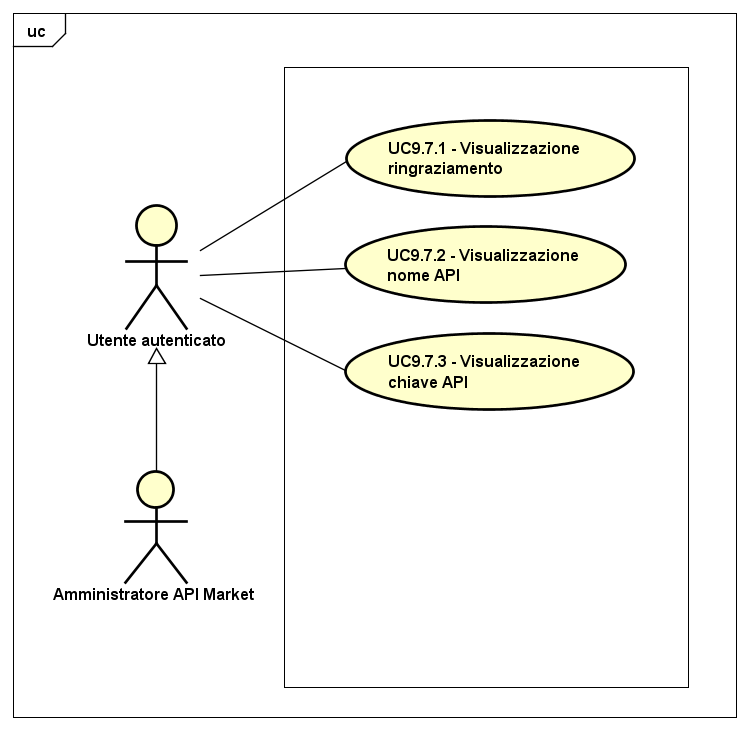
\includegraphics[scale=0.45]{UML/UC9_7.png}
	\caption{UC9.7: Riepilogo acquisto API}
\end{figure}

\begin{minipage}{\linewidth}
	\begin{tabular}{ l | p{11cm}}
		\hline
		\rowcolor{Gray}
		\multicolumn{2}{c}{UC9.7 - Riepilogo acquisto API} \\
		\hline
		\textbf{Attori} & Utente autenticato, Amministratore API Market \\
		\textbf{Descrizione} & L'attore conferma l'acquisto dell'API, portando a termine la transazione e visualizzando un messaggio di ringraziamento \\
		\textbf{Pre-Condizioni} & L'attore ha confermato l'acquisto per l'API \\
		\textbf{Post-Condizioni} & L'attore ha visualizzato il riepilogo dell'acquisto appena realizzato \\
		\textbf{Scenario Principale} & 
		\begin{enumerate*}[label=(\arabic*.),itemjoin={\newline}]
			\item L'attore può visualizzare un messaggio di ringraziamento (UC9.7.1)
			\item L'attore può visualizzare il nome dell'API appena acquistata (UC9.7.2)
			\item L'attore può visualizzare la chiave dell'API appena acquistata (UC9.7.3)
		\end{enumerate*}\\
	\end{tabular}
\end{minipage}

\paragraph{Caso d'uso UC9.7.1: Visualizzazione ringraziamento}
\label{UC9_7_1}

\begin{minipage}{\linewidth}
	\begin{tabular}{ l | p{11cm}}
		\hline
		\rowcolor{Gray}
		\multicolumn{2}{c}{UC9.7.1 - Visualizzazione ringraziamento} \\
		\hline
		\textbf{Attori} & Utente autenticato, Amministratore API Market \\
		\textbf{Descrizione} & L'attore visualizza un messaggio di ringraziamento \\
		\textbf{Pre-Condizioni} & L'attore si trova nella schermata di riepilogo acquisto dell'API \\
		\textbf{Post-Condizioni} & L'attore ha visualizzato un messaggio di ringraziamento \\
		\textbf{Scenario Principale} & 
		\begin{enumerate*}[label=(\arabic*.),itemjoin={\newline}]
			\item L'attore può visualizzare un messaggio di ringraziamento
		\end{enumerate*}\\
	\end{tabular}
\end{minipage}

\paragraph{Caso d'uso UC9.7.2: Visualizzazione nome API acquistata}
\label{UC9_7_2}

\begin{minipage}{\linewidth}
	\begin{tabular}{ l | p{11cm}}
		\hline
		\rowcolor{Gray}
		\multicolumn{2}{c}{UC9.7.2 - Visualizzazione nome API acquistata} \\
		\hline
		\textbf{Attori} & Utente autenticato, Amministratore API Market \\
		\textbf{Descrizione} & L'attore visualizza il nome dell'API acquistata \\
		\textbf{Pre-Condizioni} & L'attore si trova nella schermata di riepilogo acquisto dell'API \\
		\textbf{Post-Condizioni} & L'attore ha visualizzato il nome dell'API acquistata \\
		\textbf{Scenario Principale} & 
		\begin{enumerate*}[label=(\arabic*.),itemjoin={\newline}]
			\item L'attore può visualizzare il nome dell'API acquistata
		\end{enumerate*}\\
	\end{tabular}
\end{minipage}

\paragraph{Caso d'uso UC9.7.3: Visualizzazione chiave API acquistata}
\label{UC9_7_3}

\begin{minipage}{\linewidth}
	\begin{tabular}{ l | p{11cm}}
		\hline
		\rowcolor{Gray}
		\multicolumn{2}{c}{UC9.7.3 - Visualizzazione chiave API acquistata} \\
		\hline
		\textbf{Attori} & Utente autenticato, Amministratore API Market \\
		\textbf{Descrizione} & L'attore visualizza la chiave dell'API acquistata \\
		\textbf{Pre-Condizioni} & L'attore si trova nella schermata di riepilogo acquisto dell'API \\
		\textbf{Post-Condizioni} & L'attore ha visualizzato la chiave dell'API acquistata \\
		\textbf{Scenario Principale} & 
		\begin{enumerate*}[label=(\arabic*.),itemjoin={\newline}]
			\item L'attore può visualizzare la chiave dell'API acquistata
		\end{enumerate*}\\
	\end{tabular}
\end{minipage}

\paragraph{Caso d'uso UC9.8: Errore acquisto API}
\label{UC9_8}

\begin{minipage}{\linewidth}
	\begin{tabular}{ l | p{11cm}}
		\hline
		\rowcolor{Gray}
		\multicolumn{2}{c}{UC9.8 - Errore acquisto API} \\
		\hline
		\textbf{Attori} & Utente autenticato, Amministratore API Market \\
		\textbf{Descrizione} & L'attore visualizza un messaggio di errore e la transazione non avviene \\
		\textbf{Pre-Condizioni} & L'attore ha confermato l'acquisto per una API ma si è verificato un errore \\
		\textbf{Post-Condizioni} & L'attore ha visualizzato un errore relativo all'acquisto, con opportuna descrizione \\
		\textbf{Scenario Principale} & 
		\begin{enumerate*}[label=(\arabic*.),itemjoin={\newline}]
			\item L'attore può visualizzare un messaggio di errore e la transazione non avviene (E.g: L'API è in fase di cancellazione)
		\end{enumerate*}\\
	\end{tabular}
\end{minipage}
\newpage
\subsection{Caso d'uso UC10: Visualizzazione API registrate}
\label{UC10}
\begin{figure}[ht]
	\centering
	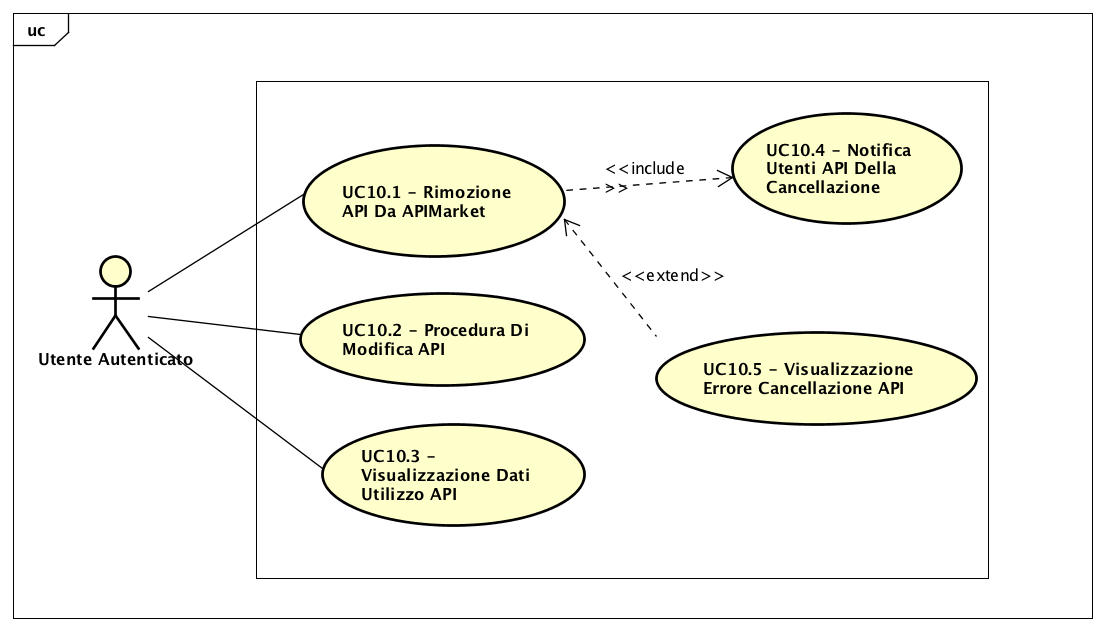
\includegraphics[scale=0.45]{UML/UC10.png}
	\caption{UC10: Visualizzazione API registrate}
\end{figure}

\begin{longtable}{ l | p{11cm}}
	\hline
	\rowcolor{Gray}
	\multicolumn{2}{c}{UC10 - Visualizzazione API registrate}\\
	\hline
	\textbf{Attori} & Utente autenticato, Amministratore API Market \\
	\textbf{Descrizione} & L'attore visualizza le API da lui registrate \\
	\textbf{Pre-Condizioni} & L'attore si trova nella schermata relativa alle API da lui registrate \\
	\textbf{Post-Condizioni} & L'attore ha visualizzato le API da lui registrate \\
	\textbf{Scenario Principale} & 
	\begin{enumerate*}[label=(\arabic*.),itemjoin={\newline}]
		\item L'attore può visualizzare il numero delle API da lui registrate (UC10.1)
		\item L'attore può visualizzare la lista delle API da lui registrate (UC10.2)
	\end{enumerate*}\\
	\textbf{Scenari Alternativi} & 
	\begin{enumerate*}[label=(\arabic*.),itemjoin={\newline}]
		\item L'attore può visualizzare i dati relativi ad ogni API (UC7)
	\end{enumerate*}\\
\end{longtable}

\subsubsection{Caso d'uso UC10.1: Visualizzazione numero API registrate}
\label{UC10_1}

\begin{minipage}{\linewidth}
	\begin{tabular}{ l | p{11cm}}
		\hline
		\rowcolor{Gray}
		\multicolumn{2}{c}{UC10.1 - Visualizzazione numero API registrate} \\
		\hline
		\textbf{Attori} & Utente autenticato, Amministratore API Market \\
		\textbf{Descrizione} & L'attore visualizza il numero di API da lui registrate \\
		\textbf{Pre-Condizioni} & L'attore si trova nella schermata relativa alle API da lui registrate \\
		\textbf{Post-Condizioni} & L'attore ha visualizzato il numero delle API da lui registrate \\
		\textbf{Scenario Principale} & 
		\begin{enumerate*}[label=(\arabic*.),itemjoin={\newline}]
			\item L'attore può visualizzare il numero di API da lui registrate
		\end{enumerate*}\\
	\end{tabular}
\end{minipage}

\newpage
\subsubsection{Caso d'uso UC10.2: Visualizzazione lista API registrate}
\label{UC10_2}
\begin{figure}[ht]
	\centering
	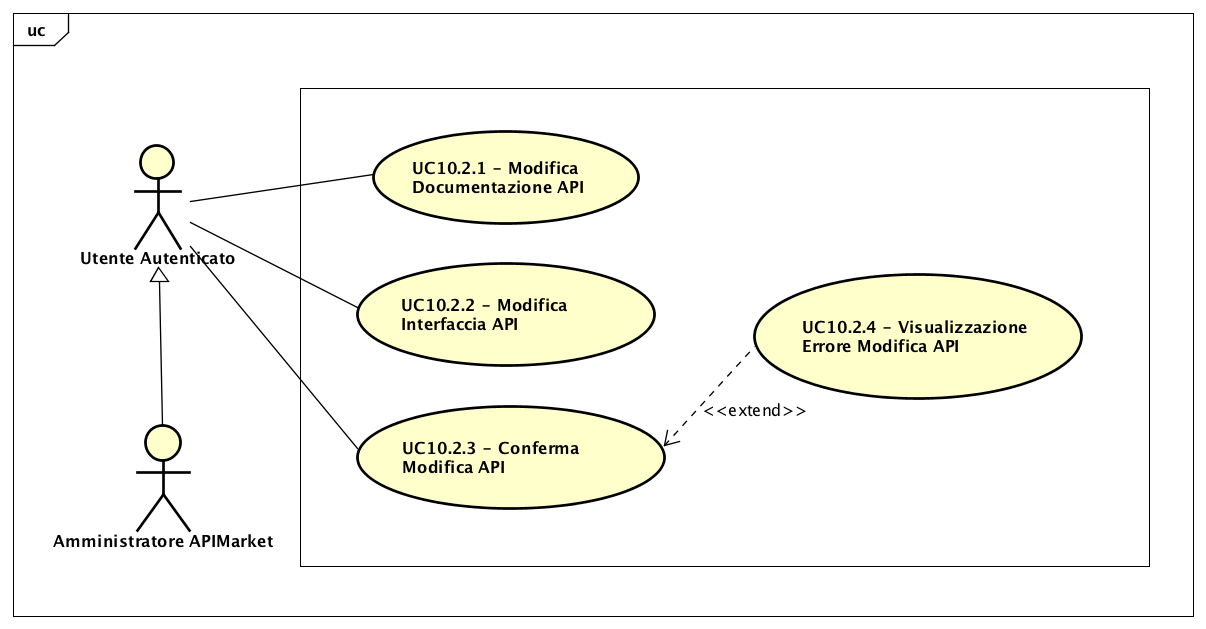
\includegraphics[scale=0.45]{UML/UC10_2.png}
	\caption{UC10.2: Visualizzazione lista API registrate}
\end{figure}

\begin{minipage}{\linewidth}
	\begin{tabular}{ l | p{11cm}}
		\hline
		\rowcolor{Gray}
		\multicolumn{2}{c}{UC10.2 - Visualizzazione lista API registrate} \\
		\hline
		\textbf{Attori} & Utente autenticato, Amministratore API Market \\
		\textbf{Descrizione} & L'attore visualizza la lista di ogni API da lui registrata \\
		\textbf{Pre-Condizioni} & L'attore si trova nella schermata relativa alle API da lui registrate \\
		\textbf{Post-Condizioni} & L'attore ha visualizzato la lista delle API da lui registrate \\
		\textbf{Scenario Principale} & 
		\begin{enumerate*}[label=(\arabic*.),itemjoin={\newline}]
			\item L'attore può visualizzare il nome di ogni API da lui registrata (UC10.2.1)
			\item L'attore può visualizzare il link alla pagina di visualizzazione API di ogni API da lui registrata (UC10.2.2)
			\item L'attore può visualizzare il numero di licenze attive di ogni API da lui registrata (UC10.2.3)
			\item L'attore può modificare ogni API da lui registrata (UC10.2.4)
			\item L'attore può eliminare ogni API da lui registrata (UC10.2.5)
		\end{enumerate*}\\
	\end{tabular}
\end{minipage}

\paragraph{Caso d'uso UC10.2.1: Visualizzazione nome API}
\label{UC10_2_1}

\begin{minipage}{\linewidth}
	\begin{tabular}{ l | p{11cm}}
		\hline
		\rowcolor{Gray}
		\multicolumn{2}{c}{UC10.2.1 - Visualizzazione nome API} \\
		\hline
		\textbf{Attori} & Utente autenticato, Amministratore API Market \\
		\textbf{Descrizione} & L'attore visualizza nella lista il nome di ogni API da lui registrata \\
		\textbf{Pre-Condizioni} & L'attore si trova nella schermata relativa alle API da lui registrate \\
		\textbf{Post-Condizioni} & L'attore ha visualizzato nella lista il nome di ogni API da lui registrata \\
		\textbf{Scenario Principale} & 
		\begin{enumerate*}[label=(\arabic*.),itemjoin={\newline}]
			\item L'attore può visualizzare nella lista il nome di ogni API da lui registrata
		\end{enumerate*}\\
	\end{tabular}
\end{minipage}

\paragraph{Caso d'uso UC10.2.2: Visualizzazione link API}
\label{UC10_2_2}

\begin{minipage}{\linewidth}
	\begin{tabular}{ l | p{11cm}}
		\hline
		\rowcolor{Gray}
		\multicolumn{2}{c}{UC10.2.2 - Visualizzazione link API} \\
		\hline
		\textbf{Attori} & Utente autenticato, Amministratore API Market \\
		\textbf{Descrizione} & L'attore visualizza nella lista il link alla visualizzazione di ogni API da lui registrata \\
		\textbf{Pre-Condizioni} & L'attore si trova nella schermata relativa alle API da lui registrate \\
		\textbf{Post-Condizioni} & L'attore ha visualizzato nella lista il link alla visualizzazione di ogni API da lui registrata \\
		\textbf{Scenario Principale} & 
		\begin{enumerate*}[label=(\arabic*.),itemjoin={\newline}]
			\item L'attore può visualizzare nella lista il link alla visualizzazione di ogni API da lui registrata
		\end{enumerate*}\\
	\end{tabular}
\end{minipage}

\paragraph{Caso d'uso UC10.2.3: Visualizzazione numero licenze attive}
\label{UC10_2_3}

\begin{minipage}{\linewidth}
	\begin{tabular}{ l | p{11cm}}
		\hline
		\rowcolor{Gray}
		\multicolumn{2}{c}{UC10.2.3 - Visualizzazione numero licenze attive} \\
		\hline
		\textbf{Attori} & Utente autenticato, Amministratore API Market \\
		\textbf{Descrizione} & L'attore visualizza nella lista il numero di licenze attive per ogni API da lui registrata \\
		\textbf{Pre-Condizioni} & L'attore si trova nella schermata relativa alle API da lui registrate \\
		\textbf{Post-Condizioni} & L'attore ha visualizzato nella lista il numero di licenze attive per ogni API da lui registrata \\
		\textbf{Scenario Principale} & 
		\begin{enumerate*}[label=(\arabic*.),itemjoin={\newline}]
			\item L'attore può visualizzare nella lista il numero di licenze attive per ogni API da lui registrata
		\end{enumerate*}\\
	\end{tabular}
\end{minipage}

\paragraph{Caso d'uso UC10.2.4: Notifica eliminazione API}
\label{UC10_2_1}

\begin{minipage}{\linewidth}
	\begin{tabular}{ l | p{11cm}}
		\hline
		\rowcolor{Gray}
		\multicolumn{2}{c}{UC10.2.1 - Notifica eliminazione API} \\
		\hline
		\textbf{Attori} & Utente autenticato, Amministratore API Market \\
		\textbf{Descrizione} & Per ogni API da lui registrata nella lista, l'attore visualizza se questa sia in fase di eliminazione \\
		\textbf{Pre-Condizioni} & L'attore si trova nella schermata relativa alle API da lui registrate \\
		\textbf{Post-Condizioni} & Per ogni API da lui registrata nella lista, l'attore ha visualizzato se questa sia in fase di eliminazione \\
		\textbf{Scenario Principale} & 
		\begin{enumerate*}[label=(\arabic*.),itemjoin={\newline}]
			\item Per ogni API da lui registrata nella lista, l'attore può visualizzare se questa sia in fase di eliminazione
		\end{enumerate*}\\
	\end{tabular}
\end{minipage}

\newpage
\paragraph{Caso d'uso UC10.2.5: Modifica API registrata}
\label{UC10_2_5}
\begin{figure}[ht]
	\centering
	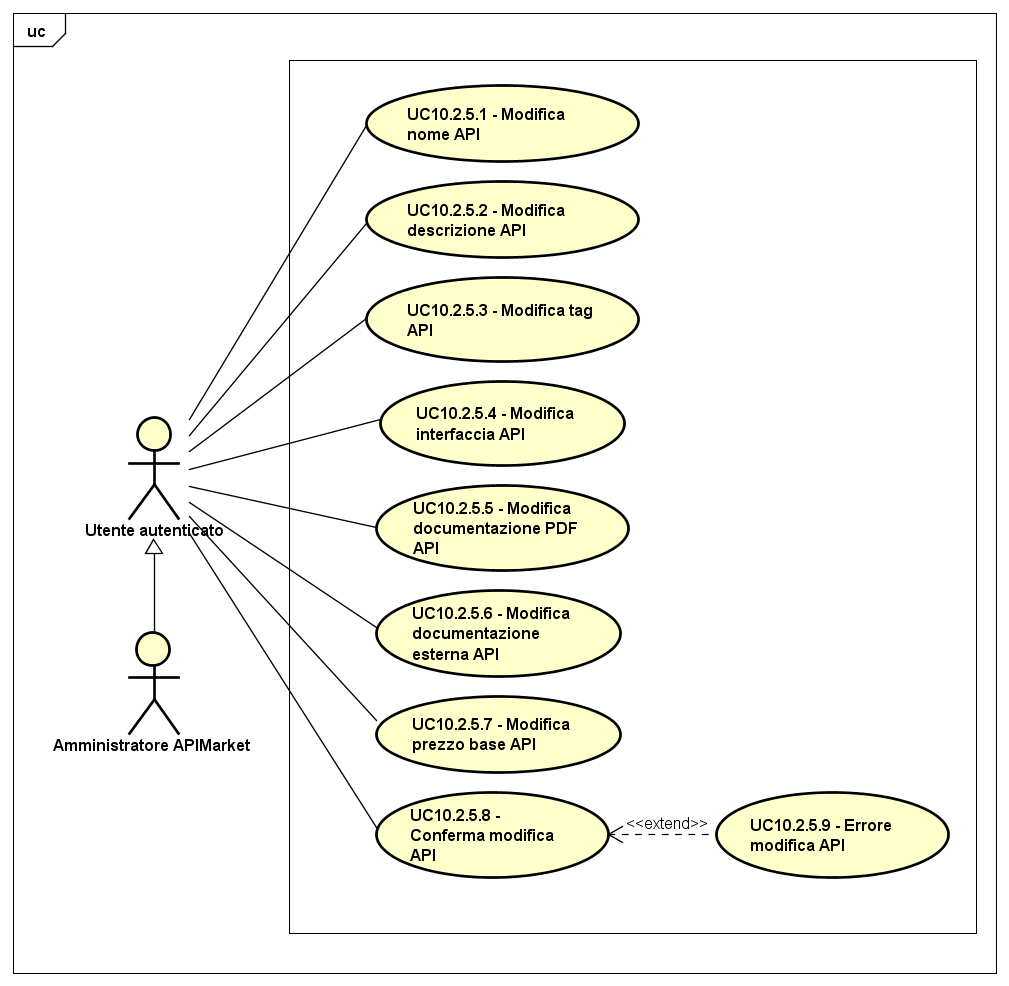
\includegraphics[scale=0.45]{UML/UC10_2_5.png}
	\caption{UC10.2.5: Modifica API registrata}
\end{figure}

\begin{minipage}{\linewidth}
	\begin{tabular}{ l | p{11cm}}
		\hline
		\rowcolor{Gray}
		\multicolumn{2}{c}{UC10.2.5 - Modifica API registrata} \\
		\hline
		\textbf{Attori} & Utente autenticato, Amministratore API Market \\
		\textbf{Descrizione} & L'attore modifica una API da lui registrata \\
		\textbf{Pre-Condizioni} & L'attore si trova nella schermata relativa alle API da lui registrate \\
		\textbf{Post-Condizioni} & L'attore ha modificato un API registrata \\
		\textbf{Scenario Principale} & 
		\begin{enumerate*}[label=(\arabic*.),itemjoin={\newline}]
			\item L'attore può modificare il nome dell'API (UC10.2.5.1)
			\item L'attore può modificare la descrizione dell'API (UC10.2.5.2)
			\item L'attore può modificare i tag dell'API (UC10.2.5.3)
			\item L'attore può modificare l'interfaccia dell'API (UC10.2.5.4)
			\item L'attore può modificare il file per la documentazione PDF (UC10.2.5.5)
			\item L'attore può modificare il link per la documentazione esterna (UC10.2.5.6)
			\item L'attore può modificare il prezzo base dell'API (UC10.2.5.7)
			\item L'attore può confermare la modifica dell'API (UC10.2.5.8)
		\end{enumerate*}\\
		\textbf{Scenari Alternativi} & 
		\begin{enumerate*}[label=(\arabic*.),itemjoin={\newline}]
			\item L'attore può visualizzare un messaggio d'errore informativo riguardo la conferma delle modifiche dell'API, e le modifiche non avvengono (UC10.2.5.9)
			\item L'attore può visualizzare un messaggio di errore riguardo al caricamento del file di documentazione PDF dell'API, ed il caricamento del file non avviene (UC10.2.5.10)
		\end{enumerate*}\\
	\end{tabular}
\end{minipage}

\subparagraph{Caso d'uso UC10.2.5.1: Modifica nome API}
\label{UC10_2_5_1}

\begin{minipage}{\linewidth}
	\begin{tabular}{ l | p{11cm}}
		\hline
		\rowcolor{Gray}
		\multicolumn{2}{c}{UC10.2.5.1 - Modifica nome API} \\
		\hline
		\textbf{Attori} & Utente autenticato, Amministratore API Market \\
		\textbf{Descrizione} & L'attore modifica il nome dell'API \\
		\textbf{Pre-Condizioni} & L'attore si trova nella schermata relativa alla modifica di una API registrata, precedentemente selezionata \\
		\textbf{Post-Condizioni} & L'attore ha modificato il nome dell'API selezionata \\
		\textbf{Scenario Principale} & 
		\begin{enumerate*}[label=(\arabic*.),itemjoin={\newline}]
			\item L'attore può modificare il nome dell'API
		\end{enumerate*}\\
	\end{tabular}
\end{minipage}

\subparagraph{Caso d'uso UC10.2.5.2: Modifica descrizione API}
\label{UC10_2_5_2}

\begin{minipage}{\linewidth}
	\begin{tabular}{ l | p{11cm}}
		\hline
		\rowcolor{Gray}
		\multicolumn{2}{c}{UC10.2.5.2 - Modifica descrizione API} \\
		\hline
		\textbf{Attori} & Utente autenticato, Amministratore API Market \\
		\textbf{Descrizione} & L'attore modifica la descrizione dell'API\\
		\textbf{Pre-Condizioni} & L'attore si trova nella schermata relativa alla modifica di una API registrata, precedentemente selezionata \\
		\textbf{Post-Condizioni} & L'attore ha modificato la descrizione dell'API selezionata \\
		\textbf{Scenario Principale} & 
		\begin{enumerate*}[label=(\arabic*.),itemjoin={\newline}]
			\item L'attore può modificare la descrizione dell'API
		\end{enumerate*}\\
	\end{tabular}
\end{minipage}

\subparagraph{Caso d'uso UC10.2.5.3: Modifica tag API}
\label{UC10_2_5_3}

\begin{minipage}{\linewidth}
	\begin{tabular}{ l | p{11cm}}
		\hline
		\rowcolor{Gray}
		\multicolumn{2}{c}{UC10.2.5.3 - Modifica tag API} \\
		\hline
		\textbf{Attori} & Utente autenticato, Amministratore API Market \\
		\textbf{Descrizione} & L'attore modifica i tag dell'API \\
		\textbf{Pre-Condizioni} & L'attore si trova nella schermata relativa alla modifica di una API registrata, precedentemente selezionata \\
		\textbf{Post-Condizioni} & L'attore ha modificato i tag dell'API selezionata \\
		\textbf{Scenario Principale} & 
		\begin{enumerate*}[label=(\arabic*.),itemjoin={\newline}]
			\item L'attore può modificare i tag dell'API
		\end{enumerate*}\\
	\end{tabular}
\end{minipage}

\subparagraph{Caso d'uso UC10.2.5.4: Modifica interfaccia API}
\label{UC10_2_5_4}

\begin{minipage}{\linewidth}
	\begin{tabular}{ l | p{11cm}}
		\hline
		\rowcolor{Gray}
		\multicolumn{2}{c}{UC10.2.5.4 - Modifica interfaccia API} \\
		\hline
		\textbf{Attori} & Utente autenticato, Amministratore API Market \\
		\textbf{Descrizione} & L'attore modifica l'interfaccia dell'API \\
		\textbf{Pre-Condizioni} & L'attore si trova nella schermata relativa alla modifica di una API registrata, precedentemente selezionata \\
		\textbf{Post-Condizioni} & L'attore ha modificato l'interfaccia pubblica dell'API selezionata \\
		\textbf{Scenario Principale} & 
		\begin{enumerate*}[label=(\arabic*.),itemjoin={\newline}]
			\item L'attore può modificare l'interfaccia dell'API
		\end{enumerate*}\\
	\end{tabular}
\end{minipage}

\subparagraph{Caso d'uso UC10.2.5.5: Modifica documentazione PDF API}
\label{UC10_2_5_5}

\begin{minipage}{\linewidth}
	\begin{tabular}{ l | p{11cm}}
		\hline
		\rowcolor{Gray}
		\multicolumn{2}{c}{UC10.2.5.5 - Modifica documentazione PDF API} \\
		\hline
		\textbf{Attori} & Utente autenticato, Amministratore API Market \\
		\textbf{Descrizione} & L'attore carica su API Market un file PDF contenente la nuova documentazione PDF dell'API \\
		\textbf{Pre-Condizioni} & L'attore si trova nella schermata relativa alla modifica di una API registrata, precedentemente selezionata \\
		\textbf{Post-Condizioni} & L'attore ha caricato su API Market un nuovo file PDF contenente la documentazione PDF dell'API \\
		\textbf{Scenario Principale} & 
		\begin{enumerate*}[label=(\arabic*.),itemjoin={\newline}]
			\item L'attore può caricare su API Market un nuovo file PDF contenente la documentazione PDF dell'API
		\end{enumerate*}\\
		\textbf{Scenari Alternativi} & 
		\begin{enumerate*}[label=(\arabic*.),itemjoin={\newline}]
			\item L'attore può visualizzare un messaggio di errore ed il caricamento del file non avviene (UC10.2.5.10)
		\end{enumerate*}\\
	\end{tabular}
\end{minipage}

\subparagraph{Caso d'uso UC10.2.5.10: Errore modifica PDF API}
\label{UC10_2_5_10}

\begin{minipage}{\linewidth}
	\begin{tabular}{ l | p{11cm}}
		\hline
		\rowcolor{Gray}
		\multicolumn{2}{c}{UC10.2.5.10 - Errore modifica PDF API} \\
		\hline
		\textbf{Attori} & Utente autenticato, Amministratore API Market \\
		\textbf{Descrizione} & L'attore visualizza un messaggio di errore e la modifica della documentazione PDF dell'API non avviene \\
		\textbf{Pre-Condizioni} & L'attore ha cercato di caricare su API Market un file contenente la documentazione dell'API ma si è verificato un errore \\
		\textbf{Post-Condizioni} & L'attore ha visualizzato un messaggio di errore \\
		\textbf{Scenario Principale} & 
		\begin{enumerate*}[label=(\arabic*.),itemjoin={\newline}]
			\item L'attore può visualizzare un messaggio di errore
		\end{enumerate*}\\
	\end{tabular}
\end{minipage}

\subparagraph{Caso d'uso UC10.2.5.6: Modifica documentazione esterna API}
\label{UC10_2_5_6}

\begin{minipage}{\linewidth}
	\begin{tabular}{ l | p{11cm}}
		\hline
		\rowcolor{Gray}
		\multicolumn{2}{c}{UC10.2.5.6 - Modifica documentazione esterna API} \\
		\hline
		\textbf{Attori} & Utente autenticato, Amministratore API Market \\
		\textbf{Descrizione} & L'attore modifica il link alla documentazione esterna dell'API \\
		\textbf{Pre-Condizioni} & L'attore si trova nella schermata relativa alla modifica di una API registrata, precedentemente selezionata \\
		\textbf{Post-Condizioni} & L'attore ha modificato il link alla documentazione esterna dell'API selezionata \\
		\textbf{Scenario Principale} & 
		\begin{enumerate*}[label=(\arabic*.),itemjoin={\newline}]
			\item L'attore può modificare il link alla documentazione esterna dell'API
		\end{enumerate*}\\
	\end{tabular}
\end{minipage}

\subparagraph{Caso d'uso UC10.2.5.7: Modifica prezzo base API}
\label{UC10_2_5_7}

\begin{minipage}{\linewidth}
	\begin{tabular}{ l | p{11cm}}
		\hline
		\rowcolor{Gray}
		\multicolumn{2}{c}{UC10.2.5.7 - Modifica prezzo base API} \\
		\hline
		\textbf{Attori} & Utente autenticato, Amministratore API Market \\
		\textbf{Descrizione} & L'attore modifica il prezzo base dell'API \\
		\textbf{Pre-Condizioni} & L'attore si trova nella schermata relativa alla modifica di una API registrata, precedentemente selezionata \\
		\textbf{Post-Condizioni} & L'attore ha modificato prezzo base dell'API selezionata \\
		\textbf{Scenario Principale} & 
		\begin{enumerate*}[label=(\arabic*.),itemjoin={\newline}]
			\item L'attore può modificare prezzo base dell'API
		\end{enumerate*}\\
	\end{tabular}
\end{minipage}

\subparagraph{Caso d'uso UC10.2.5.8: Conferma modifica API}
\label{UC10_2_5_8}

\begin{minipage}{\linewidth}
	\begin{tabular}{ l | p{11cm}}
		\hline
		\rowcolor{Gray}
		\multicolumn{2}{c}{UC10.2.5.8 - Conferma modifica API} \\
		\hline
		\textbf{Attori} & Utente autenticato, Amministratore API Market \\
		\textbf{Descrizione} & L'attore conferma le modifiche all'API, visualizzando un messaggio di successo \\
		\textbf{Pre-Condizioni} & L'attore si trova nella schermata relativa alla modifica di una API registrata, precedentemente selezionata \\
		\textbf{Post-Condizioni} & L'attore ha confermato le modifiche all'API, visualizzando un messaggio di successo \\
		\textbf{Scenario Principale} & 
		\begin{enumerate*}[label=(\arabic*.),itemjoin={\newline}]
			\item L'attore può confermare le modifiche effettuate all'API, visualizzando un messaggio di successo e venendo reindirizzato alla schermata di visualizzazione API registrate (UC10)
		\end{enumerate*}\\
	\end{tabular}
\end{minipage}

\subparagraph{Caso d'uso UC10.2.5.9: Errore modifica API}
\label{UC10_2_5_9}

\begin{minipage}{\linewidth}
	\begin{tabular}{ l | p{11cm}}
		\hline
		\rowcolor{Gray}
		\multicolumn{2}{c}{UC10.2.5.9 - Errore modifica API} \\
		\hline
		\textbf{Attori} & Utente autenticato, Amministratore API Market \\
		\textbf{Descrizione} & L'attore visualizza un messaggio di errore informativo e la modifica dell'API non avviene \\
		\textbf{Pre-Condizioni} & L'attore ha confermato la modifica di una API ma si è verificato un errore \\
		\textbf{Post-Condizioni} & L'attore ha visualizzato un messaggio di errore informativo \\
		\textbf{Scenario Principale} & 
		\begin{enumerate*}[label=(\arabic*.),itemjoin={\newline}]
			\item L'attore può visualizzare un messaggio di errore informativo e la modifica non avviene
		\end{enumerate*}\\
	\end{tabular}
\end{minipage}

\paragraph{Caso d'uso UC10.2.6: Eliminazione API registrata}
\label{UC10_2_6}

\begin{minipage}{\linewidth}
	\begin{tabular}{ l | p{11cm}}
		\hline
		\rowcolor{Gray}
		\multicolumn{2}{c}{UC10.2.6 - Eliminazione API registrata} \\
		\hline
		\textbf{Attori} & Utente autenticato, Amministratore API Market \\
		\textbf{Descrizione} & L'attore richiede l'eliminazione di una API da lui registrata, che verrà eliminata secondo le politiche di API Market \\
		\textbf{Pre-Condizioni} & L'attore si trova nella schermata relativa alle API da lui registrate \\
		\textbf{Post-Condizioni} & L'attore ha richiesto l'eliminazione di una API da lui registrata \\
		\textbf{Scenario Principale} & 
		\begin{enumerate*}[label=(\arabic*.),itemjoin={\newline}]
			\item L'attore può richiedere l'eliminazione di una API da lui registrata, che verrà eliminata secondo le politiche di API Market
		\end{enumerate*}\\
	\end{tabular}
\end{minipage}

\paragraph{Caso d'uso UC10.2.7: Revoca eliminazione API registrata}
\label{UC10_2_7}

\begin{minipage}{\linewidth}
	\begin{tabular}{ l | p{11cm}}
		\hline
		\rowcolor{Gray}
		\multicolumn{2}{c}{UC10.2.7 - Revoca eliminazione API registrata} \\
		\hline
		\textbf{Attori} & Utente autenticato, Amministratore API Market \\
		\textbf{Descrizione} & L'attore revoca la richiesta di eliminazione di una API da lui registrata \\
		\textbf{Pre-Condizioni} & L'attore si trova nella schermata relativa alle API da lui registrate \\
		\textbf{Post-Condizioni} & L'attore ha revocato la richiesta di eliminazione di una API da lui registrata \\
		\textbf{Scenario Principale} & 
		\begin{enumerate*}[label=(\arabic*.),itemjoin={\newline}]
			\item L'attore può revocare la richiesta di eliminazione di una API da lui registrata
		\end{enumerate*}\\
	\end{tabular}
\end{minipage}
\newpage
\subsection{Caso d'uso UC11 - Registrazione nuova API}
\label{UC11}
\begin{figure}[ht]
	\centering
	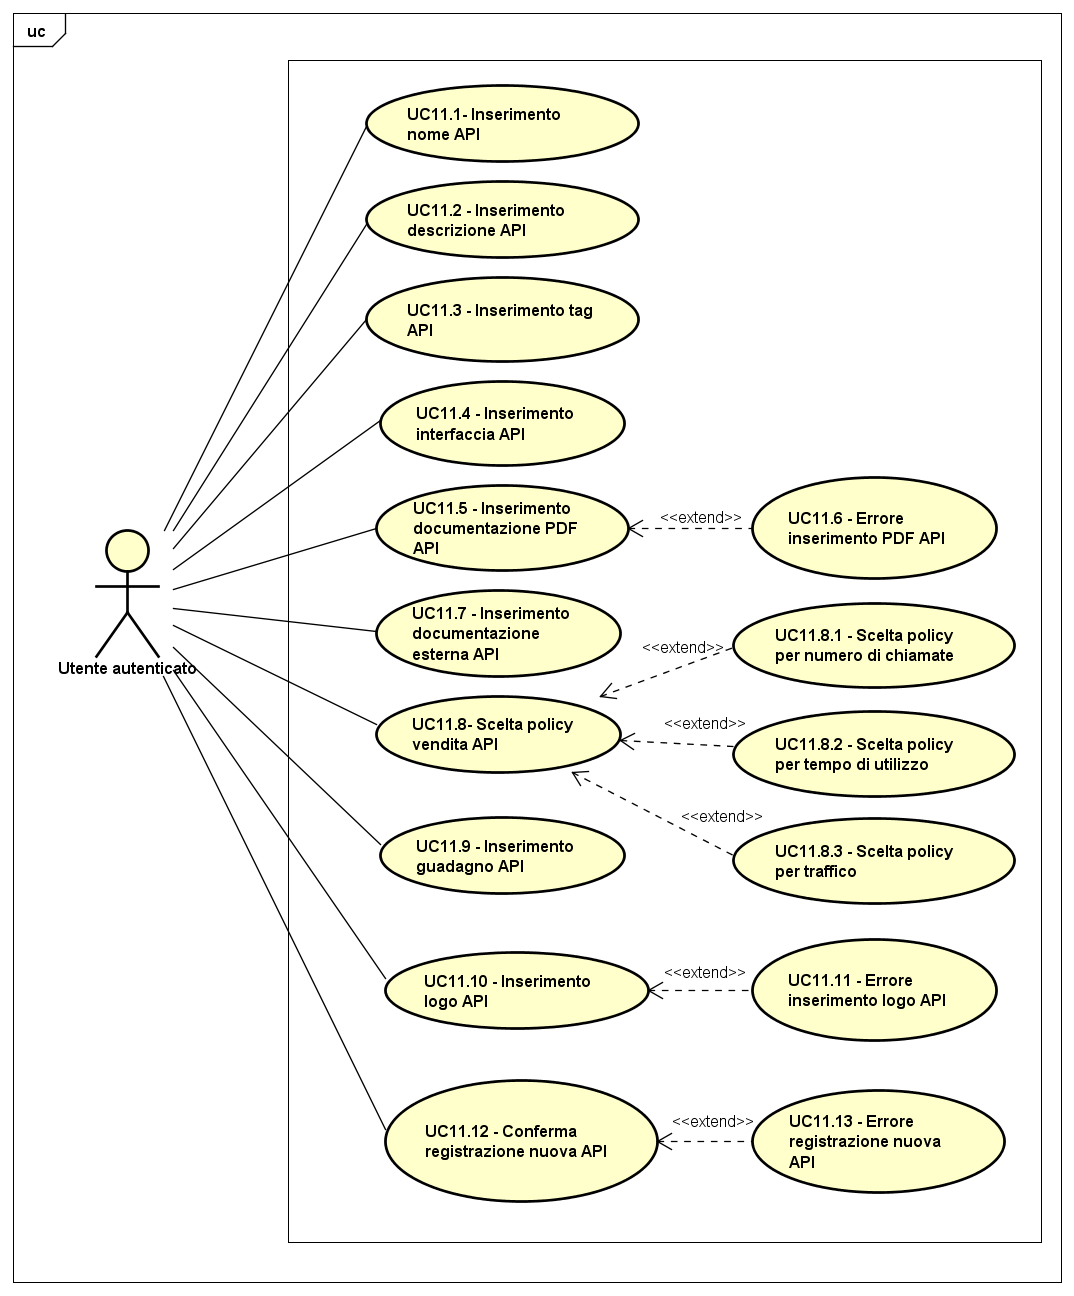
\includegraphics[scale=0.45]{UML/UC11.png}
	\caption{UC11: Registrazione nuova API}
\end{figure}

\begin{longtable}{ l | p{11cm}}
	\hline
	\rowcolor{Gray}
	\multicolumn{2}{c}{UC11 - Registrazione nuova API}\\
	\hline
	\textbf{Attori} & Utente autenticato, Amministratore API Market \\
	\textbf{Descrizione} & L'attore registra una nuova API su API Market \\
	\textbf{Pre-Condizioni} & L'attore si trova nella schermata relativa alla registrazione di una nuova API \\
	\textbf{Post-Condizioni} & L'attore ha registrato una nuova API su API Market \\
	\textbf{Scenario Principale} & 
	\begin{enumerate*}[label=(\arabic*.),itemjoin={\newline}]
		\item L'attore può inserire il nome della nuova API (UC11.1)
		\item L'attore può inserire la descrizione della nuova API (UC11.2)
		\item L'attore può inserire i tag della nuova API (UC11.3)
		\item L'attore può inserire l'interfaccia della nuova API (UC11.4)
		\item L'attore può inserire il file per la documentazione PDF della nuova API (UC11.5)
		\item L'attore può inserire il link per la documentazione esterna della nuova API (UC11.7)
		\item L'attore può inserire il prezzo base della nuova API (UC11.8)
		\item L'attore può confermare la registrazione della nuova API (UC11.9)
	\end{enumerate*}\\
	\textbf{Scenario Principale} & 
	\begin{enumerate*}[label=(\arabic*.),itemjoin={\newline}]
			\item L'attore può visualizzare un messaggio di errore riguardo al caricamento del file di documentazione PDF dell'API, ed il caricamento del file non avviene (UC11.6)
			\item L'attore può visualizzare un messaggio d'errore informativo riguardo la conferma della registrazione dell'API, e la registrazione non avviene (UC11.10)
	\end{enumerate*}\\
\end{longtable}

\subsubsection{Caso d'uso UC11.1: Inserimento nome API}
\label{UC11_1}

\begin{minipage}{\linewidth}
	\begin{tabular}{ l | p{11cm}}
		\hline
		\rowcolor{Gray}
		\multicolumn{2}{c}{UC11.1 - Inserimento nome API} \\
		\hline
		\textbf{Attori} & Utente autenticato, Amministratore API Market \\
		\textbf{Descrizione} & L'attore inserisce il nome della nuova API \\
		\textbf{Pre-Condizioni} & L'attore si trova nella schermata relativa alla registrazione di una nuova API \\
		\textbf{Post-Condizioni} & L'attore ha inserito il nome della nuova API \\
		\textbf{Scenario Principale} & 
		\begin{enumerate*}[label=(\arabic*.),itemjoin={\newline}]
			\item L'attore può inserire il nome della nuova API
		\end{enumerate*}\\
	\end{tabular}
\end{minipage}

\subsubsection{Caso d'uso UC11.2: Inserimento descrizione API}
\label{UC11_2}

\begin{minipage}{\linewidth}
	\begin{tabular}{ l | p{11cm}}
		\hline
		\rowcolor{Gray}
		\multicolumn{2}{c}{UC11.2 - Inserimento descrizione API} \\
		\hline
		\textbf{Attori} & Utente autenticato, Amministratore API Market \\
		\textbf{Descrizione} & L'attore inserisce la descrizione della nuova API \\
		\textbf{Pre-Condizioni} & L'attore si trova nella schermata relativa alla registrazione di una nuova API \\
		\textbf{Post-Condizioni} & L'attore ha inserito la descrizione della nuova API \\
		\textbf{Scenario Principale} & 
		\begin{enumerate*}[label=(\arabic*.),itemjoin={\newline}]
			\item L'attore può inserire la descrizione della nuova API
		\end{enumerate*}\\
	\end{tabular}
\end{minipage}

\subsubsection{Caso d'uso UC11.3: Inserimento tag API}
\label{UC11_3}

\begin{minipage}{\linewidth}
	\begin{tabular}{ l | p{11cm}}
		\hline
		\rowcolor{Gray}
		\multicolumn{2}{c}{UC11.3 - Inserimento tag API} \\
		\hline
		\textbf{Attori} & Utente autenticato, Amministratore API Market \\
		\textbf{Descrizione} & L'attore inserisce i tag della nuova API \\
		\textbf{Pre-Condizioni} & L'attore si trova nella schermata relativa alla registrazione di una nuova API \\
		\textbf{Post-Condizioni} & L'attore ha inserito i tag della nuova API \\
		\textbf{Scenario Principale} & 
		\begin{enumerate*}[label=(\arabic*.),itemjoin={\newline}]
			\item L'attore può inserire i tag della nuova API
		\end{enumerate*}\\
	\end{tabular}
\end{minipage}

\subsubsection{Caso d'uso UC11.4: Inserimento interfaccia API}
\label{UC11_4}

\begin{minipage}{\linewidth}
	\begin{tabular}{ l | p{11cm}}
		\hline
		\rowcolor{Gray}
		\multicolumn{2}{c}{UC11.4 - Inserimento interfaccia API} \\
		\hline
		\textbf{Attori} & Utente autenticato, Amministratore API Market \\
		\textbf{Descrizione} & L'attore inserisce l'interfaccia della nuova API \\
		\textbf{Pre-Condizioni} & L'attore si trova nella schermata relativa alla registrazione di una nuova API \\
		\textbf{Post-Condizioni} & L'attore ha inserito l'interfaccia della nuova API \\
		\textbf{Scenario Principale} & 
		\begin{enumerate*}[label=(\arabic*.),itemjoin={\newline}]
			\item L'attore può inserire l'interfaccia della nuova API
		\end{enumerate*}\\
	\end{tabular}
\end{minipage}

\subsubsection{Caso d'uso UC11.5: Inserimento documentazione PDF API}
\label{UC11_5}

\begin{minipage}{\linewidth}
	\begin{tabular}{ l | p{11cm}}
		\hline
		\rowcolor{Gray}
		\multicolumn{2}{c}{UC11.5 - Inserimento documentazione PDF API} \\
		\hline
		\textbf{Attori} & Utente autenticato, Amministratore API Market \\
		\textbf{Descrizione} & L'attore carica su API Market un file PDF contenente la documentazione PDF della nuova API \\
		\textbf{Pre-Condizioni} & L'attore si trova nella schermata relativa alla registrazione di una nuova API \\
		\textbf{Post-Condizioni} & L'attore ha caricato su API Market un file PDF contenente la documentazione PDF della nuova API \\
		\textbf{Scenario Principale} & 
		\begin{enumerate*}[label=(\arabic*.),itemjoin={\newline}]
			\item L'attore può caricare su API Market un file PDF contenente la documentazione PDF della nuova API
		\end{enumerate*}\\
		\textbf{Scenari Alternativi} & 
		\begin{enumerate*}[label=(\arabic*.),itemjoin={\newline}]
		\item L'attore può visualizzare un messaggio di errore ed il caricamento del file non avviene (UC11.10)
		\end{enumerate*}\\
	\end{tabular}
\end{minipage}

\subsubsection{Caso d'uso UC11.6: Errore inserimento PDF API}
\label{UC11_6}

\begin{minipage}{\linewidth}
	\begin{tabular}{ l | p{11cm}}
		\hline
		\rowcolor{Gray}
		\multicolumn{2}{c}{UC11.6 - Errore inserimento PDF API} \\
		\hline
		\textbf{Attori} & Utente autenticato, Amministratore API Market \\
		\textbf{Descrizione} & L'attore visualizza un messaggio di errore e l'inserimento della documentazione PDF della nuova API non avviene \\
		\textbf{Pre-Condizioni} & L'attore ha cercato di caricare su API Market un file contenente la documentazione della nuova API ma si è verificato un errore \\
		\textbf{Post-Condizioni} & L'attore ha visualizzato un messaggio di errore \\
		\textbf{Scenario Principale} & 
		\begin{enumerate*}[label=(\arabic*.),itemjoin={\newline}]
			\item L'attore può visualizzare un messaggio di errore
		\end{enumerate*}\\
	\end{tabular}
\end{minipage}

\subsubsection{Caso d'uso UC11.7: Inserimento documentazione esterna API}
\label{UC11_7}

\begin{minipage}{\linewidth}
	\begin{tabular}{ l | p{11cm}}
		\hline
		\rowcolor{Gray}
		\multicolumn{2}{c}{UC11.7 - Inserimento documentazione esterna API} \\
		\hline
		\textbf{Attori} & Utente autenticato, Amministratore API Market \\
		\textbf{Descrizione} & L'attore inserisce il link alla documentazione esterna della nuova API \\
		\textbf{Pre-Condizioni} & L'attore si trova nella schermata relativa alla registrazione di una nuova API \\
		\textbf{Post-Condizioni} & L'attore ha inserito il link alla documentazione esterna della nuova API \\
		\textbf{Scenario Principale} & 
		\begin{enumerate*}[label=(\arabic*.),itemjoin={\newline}]
			\item L'attore può inserire il link alla documentazione esterna della nuova API
		\end{enumerate*}\\
	\end{tabular}
\end{minipage}

\subsubsection{Caso d'uso UC11.8: Inserimento prezzo base API}
\label{UC11_8}

\begin{minipage}{\linewidth}
	\begin{tabular}{ l | p{11cm}}
		\hline
		\rowcolor{Gray}
		\multicolumn{2}{c}{UC11.8 - Inserimento prezzo base API} \\
		\hline
		\textbf{Attori} & Utente autenticato, Amministratore API Market \\
		\textbf{Descrizione} & L'attore inserisce il prezzo base della nuova API \\
		\textbf{Pre-Condizioni} & L'attore si trova nella schermata relativa alla registrazione di una nuova API \\
		\textbf{Post-Condizioni} & L'attore ha inserito il prezzo base della nuova API \\
		\textbf{Scenario Principale} & 
		\begin{enumerate*}[label=(\arabic*.),itemjoin={\newline}]
			\item L'attore può inserire il prezzo base della nuova API
		\end{enumerate*}\\
	\end{tabular}
\end{minipage}

\subsubsection{Caso d'uso UC11.9: Conferma registrazione nuova API}
\label{UC11_9}

\begin{minipage}{\linewidth}
	\begin{tabular}{ l | p{11cm}}
		\hline
		\rowcolor{Gray}
		\multicolumn{2}{c}{UC11.9 - Conferma registrazione nuova API} \\
		\hline
		\textbf{Attori} & Utente autenticato, Amministratore API Market \\
		\textbf{Descrizione} & L'attore conferma la registrazione della nuova API \\
		\textbf{Pre-Condizioni} & L'attore si trova nella schermata relativa alla registrazione di una nuova API \\
		\textbf{Post-Condizioni} & L'attore ha confermato la registrazione della nuova API \\
		\textbf{Scenario Principale} & 
		\begin{enumerate*}[label=(\arabic*.),itemjoin={\newline}]
			\item L'attore può confermare la registrazione della nuova API, visualizzando un messaggio di successo e venendo reindirizzato alla schermata di visualizzazione API registrate (UC10)
		\end{enumerate*}\\
	\end{tabular}
\end{minipage}

\subsubsection{Caso d'uso UC11.10: Errore registrazione nuova API}
\label{UC11_10}

\begin{minipage}{\linewidth}
	\begin{tabular}{ l | p{11cm}}
		\hline
		\rowcolor{Gray}
		\multicolumn{2}{c}{UC11.10 - Errore registrazione nuova API} \\
		\hline
		\textbf{Attori} & Utente autenticato, Amministratore API Market \\
		\textbf{Descrizione} & L'attore visualizza un messaggio di errore informativo e la registrazione della nuova API non avviene \\
		\textbf{Pre-Condizioni} & L'attore ha confermato la registrazione della una nuova API ma si è verificato un errore \\
		\textbf{Post-Condizioni} & L'attore ha visualizzato un messaggio di errore informativo \\
		\textbf{Scenario Principale} & 
		\begin{enumerate*}[label=(\arabic*.),itemjoin={\newline}]
			\item L'attore può visualizzare un messaggio di errore informativo e la registrazione della nuova API non avviene
		\end{enumerate*}\\
	\end{tabular}
\end{minipage}
\newpage
\subsection{Caso d'uso UC12: Gestione proprio profilo utente}
\label{UC12}
\begin{figure}[ht]
	\centering
	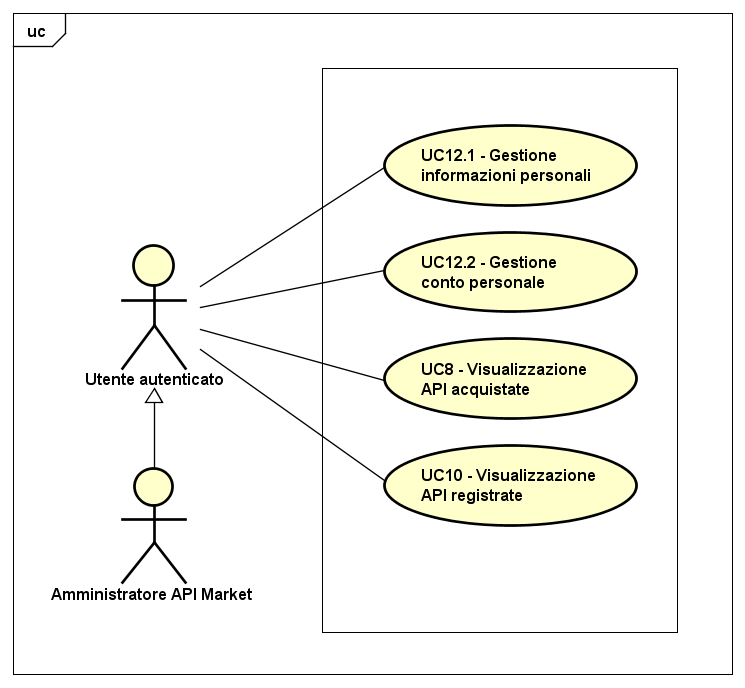
\includegraphics[scale=0.45]{UML/UC12.png}
	\caption{UC12 - Gestione proprio profilo utente}
\end{figure}

\begin{longtable}{ l | p{11cm}}
	\hline
	\rowcolor{Gray}
	\multicolumn{2}{c}{UC12 - Gestione proprio profilo utente} \\
	\hline
	\textbf{Attori} & Cliente, Sviluppatore \\
	\textbf{Descrizione} & L'attore visualizza e/o gestisce le informazioni del proprio profilo utente \\
	\textbf{Pre-Condizioni} & L'attore si trova nella schermata relativa alla gestione del proprio profilo utente \\
	\textbf{Post-Condizioni} & L'attore ha visualizzato e/o gestito le informazioni del proprio profilo utente \\
	\textbf{Scenario Principale} & 
	\begin{enumerate*}[label=(\arabic*.),itemjoin={\newline}]
		\item L'attore può gestire le proprie informazioni personali (UC12.1)
		\item L'attore può gestire il proprio conto utente (UC12.2)
		\item L'attore può visualizzare le API da lui acquistate (UC8)
		\item Lo sviluppatore può visualizzare le API da lui registrate (UC10)
	\end{enumerate*}\\
\end{longtable}

\newpage
\subsubsection{Caso d'uso UC12.1: Gestione informazioni personali}
\label{UC12_1}
\begin{figure}[ht]
	\centering
	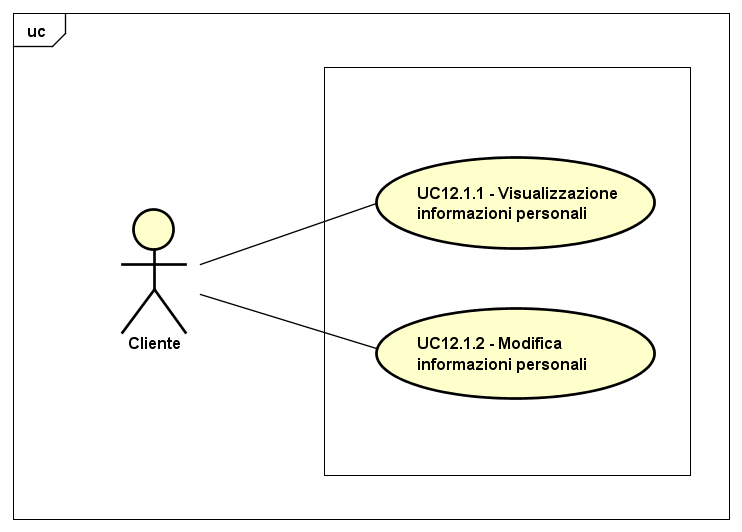
\includegraphics[scale=0.45]{UML/UC12_1.png}
	\caption{UC12.1: Gestione informazioni personali}
\end{figure}

\begin{minipage}{\linewidth}
	\begin{tabular}{ l | p{11cm}}
		\hline
		\rowcolor{Gray}
		\multicolumn{2}{c}{UC12.1 - Gestione informazioni personali} \\
		\hline
		\textbf{Attori} & Cliente \\
		\textbf{Descrizione} & L'attore visualizza e/o modifica le proprie informazioni personali \\
		\textbf{Pre-Condizioni} & L'attore si trova nella schermata relativa alla gestione del proprio profilo utente \\
		\textbf{Post-Condizioni} & L'attore ha visualizzato e/o modificato le proprie informazioni personali \\
		\textbf{Scenario Principale} & 
		\begin{enumerate*}[label=(\arabic*.),itemjoin={\newline}]
			\item L'attore può visualizzare le proprie informazioni personali (UC12.1.1)
			\item L'attore può modificare le proprie informazioni personali (UC12.1.2)
		\end{enumerate*}
	\end{tabular}
\end{minipage}

\newpage
\paragraph{Caso d'uso UC12.1.1: Visualizzazione informazioni personali}
\label{UC12_1_1}
\begin{figure}[ht]
	\centering
	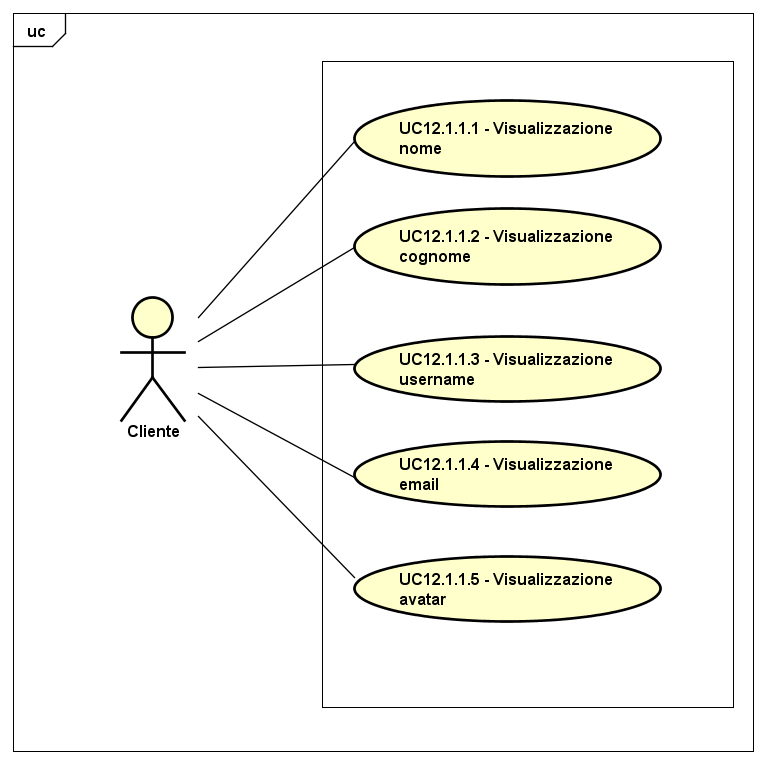
\includegraphics[scale=0.45]{UML/UC12_1_1.png}
	\caption{UC12.1.1: Visualizzazione informazioni personali}
\end{figure}

\begin{minipage}{\linewidth}
\begin{tabular}{ l | p{11cm}}
	\hline
	\rowcolor{Gray}
	\multicolumn{2}{c}{UC12.1.1 - Visualizzazione informazioni personali} \\
	\hline
	\textbf{Attori} & Cliente \\
	\textbf{Descrizione} & L'attore visualizza le proprie informazioni personali \\
	\textbf{Pre-Condizioni} & L'attore si trova nella schermata relativa alla gestione del proprio profilo utente \\
	\textbf{Post-Condizioni} & L'attore ha visualizzato le proprie informazioni personali \\
	\textbf{Scenario Principale} & 
	\begin{enumerate*}[label=(\arabic*.),itemjoin={\newline}]
		\item L'attore può visualizzare il proprio nome (UC12.1.1.1)
		\item L'attore può visualizzare il proprio cognome (UC12.1.1.2)
		\item L'attore può visualizzare il proprio username (UC12.1.1.3)
		\item L'attore può visualizzare la propria email (UC12.1.1.4)
		\item L'attore può visualizzare il proprio avatar (UC12.1.1.5)
		\item L'attore può visualizzare la tipologia del proprio account (UC12.1.1.6)
	\end{enumerate*}\\
\end{tabular}
\end{minipage}

\subparagraph{Caso d'uso UC12.1.1.1: Visualizzazione nome}
\label{UC12_1_1_1}

\begin{minipage}{\linewidth}
\begin{tabular}{ l | p{11cm}}
	\hline
	\rowcolor{Gray}
	\multicolumn{2}{c}{UC12.1.1.1 - Visualizzazione nome} \\
	\hline
	\textbf{Attori} & Cliente \\
	\textbf{Descrizione} & L'attore visualizzare il proprio nome \\
	\textbf{Pre-Condizioni} & L'attore si trova nella schermata relativa alla gestione delle informazioni personali \\
	\textbf{Post-Condizioni} & L'attore ha visualizzato il proprio nome \\
	\textbf{Scenario Principale} & 
	\begin{enumerate*}[label=(\arabic*.),itemjoin={\newline}]
		\item L'attore può visualizzare il proprio nome
	\end{enumerate*}
\end{tabular}
\end{minipage}

\subparagraph{Caso d'uso UC12.1.1.2: Visualizzazione cognome}
\label{UC12_1_1_2}

\begin{minipage}{\linewidth}
	\begin{tabular}{ l | p{11cm}}
		\hline
		\rowcolor{Gray}
		\multicolumn{2}{c}{UC12.1.1.2 - Visualizzazione cognome} \\
		\hline
		\textbf{Attori} & Cliente \\
		\textbf{Descrizione} & L'attore visualizzare il proprio cognome \\
	\textbf{Pre-Condizioni} & L'attore si trova nella schermata relativa alla gestione delle informazioni personali \\
	\textbf{Post-Condizioni} & L'attore ha visualizzato il proprio cognome \\
	\textbf{Scenario Principale} & 
	\begin{enumerate*}[label=(\arabic*.),itemjoin={\newline}]
		\item L'attore può visualizzare il proprio cognome
	\end{enumerate*}
	\end{tabular}
\end{minipage}

\subparagraph{Caso d'uso UC12.1.1.3: Visualizzazione username}
\label{UC12_1_1_3}

\begin{minipage}{\linewidth}
	\begin{tabular}{ l | p{11cm}}
		\hline
		\rowcolor{Gray}
		\multicolumn{2}{c}{UC12.1.1.3 - Visualizzazione username} \\
		\hline
		\textbf{Attori} & Cliente \\
		\textbf{Descrizione} & L'attore visualizzare il proprio username \\
	\textbf{Pre-Condizioni} & L'attore si trova nella schermata relativa alla gestione delle informazioni personali \\
	\textbf{Post-Condizioni} & L'attore ha visualizzato il proprio username \\
	\textbf{Scenario Principale} & 
	\begin{enumerate*}[label=(\arabic*.),itemjoin={\newline}]
		\item L'attore può visualizzare il proprio username
	\end{enumerate*}
	\end{tabular}
\end{minipage}

\subparagraph{Caso d'uso UC12.1.1.4: Visualizzazione email}
\label{UC12_1_1_4}

\begin{minipage}{\linewidth}
	\begin{tabular}{ l | p{11cm}}
		\hline
		\rowcolor{Gray}
		\multicolumn{2}{c}{UC12.1.1.4 - Visualizzazione email} \\
		\hline
		\textbf{Attori} & Cliente \\
		\textbf{Descrizione} & L'attore visualizzare la propria email \\
		\textbf{Pre-Condizioni} & L'attore si trova nella schermata relativa alla gestione delle informazioni personali \\
		\textbf{Post-Condizioni} & L'attore ha visualizzato la propria email \\
		\textbf{Scenario Principale} & 
		\begin{enumerate*}[label=(\arabic*.),itemjoin={\newline}]
			\item L'attore può visualizzare la propria email
		\end{enumerate*}
	\end{tabular}
\end{minipage}

\subparagraph{Caso d'uso UC12.1.1.5: Visualizzazione avatar}
\label{UC12_1_1_5}

\begin{minipage}{\linewidth}
	\begin{tabular}{ l | p{11cm}}
		\hline
		\rowcolor{Gray}
		\multicolumn{2}{c}{UC12.1.1.5 - Visualizzazione avatar} \\
		\hline
		\textbf{Attori} & Cliente \\
		\textbf{Descrizione} & L'attore visualizzare il proprio avatar \\
		\textbf{Pre-Condizioni} & L'attore si trova nella schermata relativa alla gestione delle informazioni personali \\
		\textbf{Post-Condizioni} & L'attore ha visualizzato il proprio avatar \\
		\textbf{Scenario Principale} & 
		\begin{enumerate*}[label=(\arabic*.),itemjoin={\newline}]
			\item L'attore può visualizzare il proprio avatar
		\end{enumerate*}
	\end{tabular}
\end{minipage}

\subparagraph{Caso d'uso UC12.1.1.6: Visualizzazione tipologia account}
\label{UC12_1_1_6}

\begin{minipage}{\linewidth}
	\begin{tabular}{ l | p{11cm}}
		\hline
		\rowcolor{Gray}
		\multicolumn{2}{c}{UC12.1.1.6 - Visualizzazione tipologia account} \\
		\hline
		\textbf{Attori} & Cliente \\
		\textbf{Descrizione} & L'attore visualizzare la tipologia del proprio account \\
		\textbf{Pre-Condizioni} & L'attore si trova nella schermata relativa alla gestione delle informazioni personali \\
		\textbf{Post-Condizioni} & L'attore ha visualizzato la tipologia del proprio account \\
		\textbf{Scenario Principale} & 
		\begin{enumerate*}[label=(\arabic*.),itemjoin={\newline}]
			\item L'attore può visualizzare la tipologia del proprio account
		\end{enumerate*}
	\end{tabular}
\end{minipage}

\newpage
\paragraph{Caso d'uso UC12.1.2: Modifica informazioni personali}
\label{UC12_1_2}
\begin{figure}[ht]
	\centering
	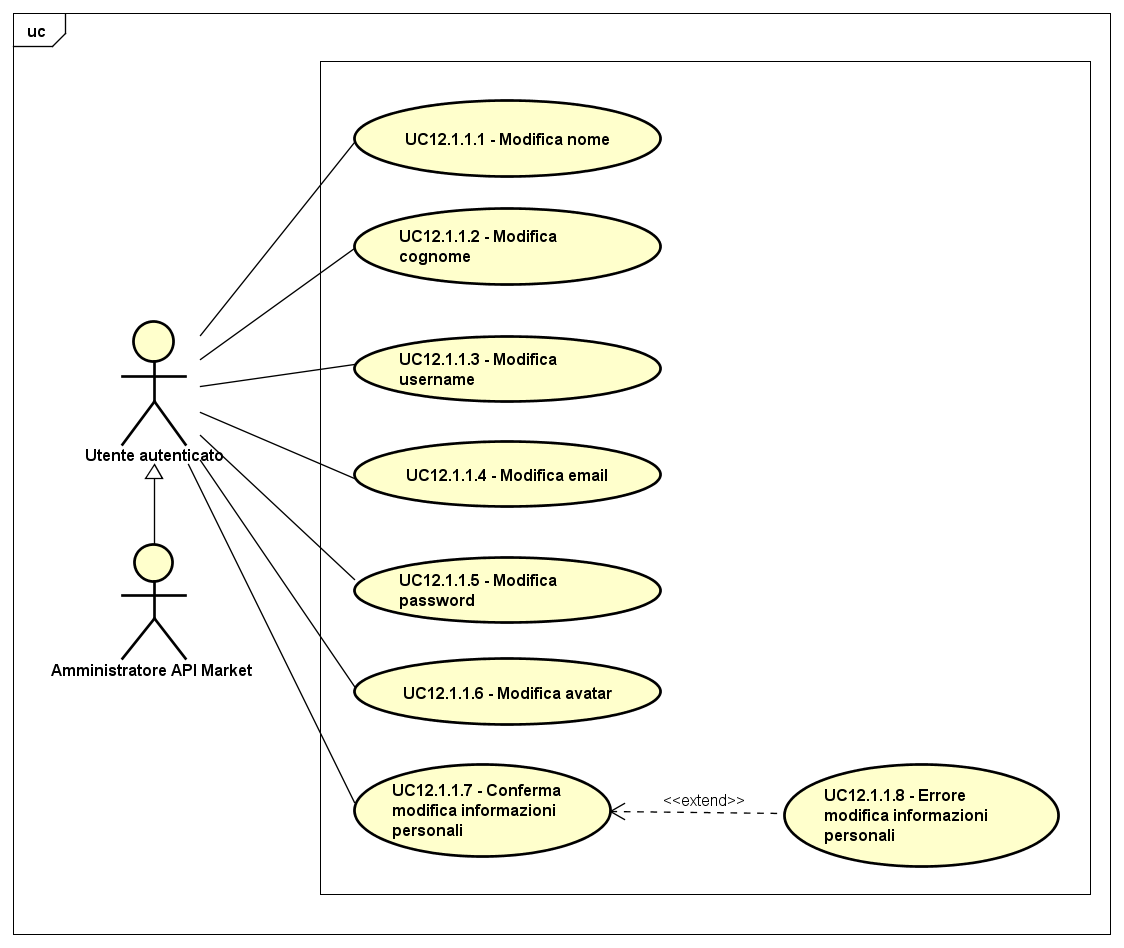
\includegraphics[scale=0.45]{UML/UC12_1_2.png}
	\caption{UC12.1.2: Modifica informazioni personali}
\end{figure}

\begin{tabular}{ l | p{11cm}}
	\hline
	\rowcolor{Gray}
	\multicolumn{2}{c}{UC12.1.2 - Modifica informazioni personali} \\
	\hline
	\textbf{Attori} & Cliente \\
	\textbf{Descrizione} & L'attore modifica le proprie informazioni personali \\
	\textbf{Pre-Condizioni} & L'attore si trova nella schermata relativa alla gestione del proprio profilo utente \\
	\textbf{Post-Condizioni} & L'attore ha modificato le proprie informazioni personali \\
	\textbf{Scenario Principale} & 
	\begin{enumerate*}[label=(\arabic*.),itemjoin={\newline}]
		\item L'attore può modificare il proprio nome (UC12.1.2.1)
		\item L'attore può modificare il proprio cognome (UC12.1.2.2)
		\item L'attore può modificare il proprio username (UC12.1.2.3)
		\item L'attore può modificare la propria email (UC12.1.2.4)
		\item L'attore può modificare la propria password (UC12.1.2.5)
		\item L'attore può modificare il proprio avatar (UC12.1.2.6)
		\item L'attore può confermare la modifica alle proprie informazioni personali (UC12.1.2.7)
		\item L'attore può migliorare il proprio status a sviluppatore (UC12.1.2.9)
	\end{enumerate*}\\
	\textbf{Scenari Alternativi} & 
	\begin{enumerate*}[label=(\arabic*.),itemjoin={\newline}]
		\item L'attore, dopo aver confermato le modifiche alle proprie informazioni personali, può visualizzare un messaggio di errore informativo (E.g: dati non validi, formati dei file errati), e le modifiche non avvengono (UC12.1.2.8)
	\end{enumerate*}\\
\end{tabular}

\subparagraph{Caso d'uso UC12.1.2.1: Modifica nome}
\label{UC12_1_2_1}

\begin{minipage}{\linewidth}
	\begin{tabular}{ l | p{11cm}}
		\hline
		\rowcolor{Gray}
		\multicolumn{2}{c}{UC12.1.2.1 - Modifica nome} \\
		\hline
		\textbf{Attori} & Cliente \\
		\textbf{Descrizione} & L'attore modifica il proprio nome \\
		\textbf{Pre-Condizioni} & L'attore si trova nella schermata relativa alla gestione delle informazioni personali \\
		\textbf{Post-Condizioni} & L'attore ha modificato il proprio nome \\
		\textbf{Scenario Principale} & 
		\begin{enumerate*}[label=(\arabic*.),itemjoin={\newline}]
			\item L'attore può modificare il proprio nome
		\end{enumerate*}
	\end{tabular}
\end{minipage}

\subparagraph{Caso d'uso UC12.1.2.2: Modifica cognome}
\label{UC12_1_2_2}

\begin{minipage}{\linewidth}
	\begin{tabular}{ l | p{11cm}}
		\hline
		\rowcolor{Gray}
		\multicolumn{2}{c}{UC12.1.2.2 - Modifica cognome} \\
		\hline
		\textbf{Attori} & Cliente \\
		\textbf{Descrizione} & L'attore modifica il proprio cognome \\
		\textbf{Pre-Condizioni} & L'attore si trova nella schermata relativa alla gestione delle informazioni personali \\
		\textbf{Post-Condizioni} & L'attore ha modificato il proprio cognome \\
		\textbf{Scenario Principale} & 
		\begin{enumerate*}[label=(\arabic*.),itemjoin={\newline}]
			\item L'attore può modificare il proprio cognome
		\end{enumerate*}
	\end{tabular}
\end{minipage}

\subparagraph{Caso d'uso UC12.1.2.3: Modifica username}
\label{UC12_1_2_3}

\begin{minipage}{\linewidth}
	\begin{tabular}{ l | p{11cm}}
		\hline
		\rowcolor{Gray}
		\multicolumn{2}{c}{UC12.1.2.3 - Modifica username} \\
		\hline
		\textbf{Attori} & Cliente \\
		\textbf{Descrizione} & L'attore modifica il proprio username \\
		\textbf{Pre-Condizioni} & L'attore si trova nella schermata relativa alla gestione delle informazioni personali \\
		\textbf{Post-Condizioni} & L'attore ha modificato il proprio username \\
		\textbf{Scenario Principale} & 
		\begin{enumerate*}[label=(\arabic*.),itemjoin={\newline}]
			\item L'attore può modificare il proprio username
		\end{enumerate*}
	\end{tabular}
\end{minipage}

\subparagraph{Caso d'uso UC12.1.2.4: Modifica email}
\label{UC12_1_2_4}

\begin{minipage}{\linewidth}
	\begin{tabular}{ l | p{11cm}}
		\hline
		\rowcolor{Gray}
		\multicolumn{2}{c}{UC12.1.2.4 - Modifica email} \\
		\hline
		\textbf{Attori} & Cliente \\
		\textbf{Descrizione} & L'attore modifica la propria email \\
		\textbf{Pre-Condizioni} & L'attore si trova nella schermata relativa alla gestione delle informazioni personali \\
		\textbf{Post-Condizioni} & L'attore ha modificato la propria email \\
		\textbf{Scenario Principale} & 
		\begin{enumerate*}[label=(\arabic*.),itemjoin={\newline}]
			\item L'attore può modificare la propria email
		\end{enumerate*}
	\end{tabular}
\end{minipage}

\subparagraph{Caso d'uso UC12.1.2.5: Modifica password}
\label{UC12_1_2_5}

\begin{minipage}{\linewidth}
	\begin{tabular}{ l | p{11cm}}
		\hline
		\rowcolor{Gray}
		\multicolumn{2}{c}{UC12.1.2.5 - Modifica password} \\
		\hline
		\textbf{Attori} & Cliente \\
		\textbf{Descrizione} & L'attore modifica la propria password \\
		\textbf{Pre-Condizioni} & L'attore si trova nella schermata relativa alla gestione delle informazioni personali \\
		\textbf{Post-Condizioni} & L'attore ha modificato la propria password \\
		\textbf{Scenario Principale} & 
		\begin{enumerate*}[label=(\arabic*.),itemjoin={\newline}]
			\item L'attore può modificare la propria password
		\end{enumerate*}
	\end{tabular}
\end{minipage}

\subparagraph{Caso d'uso UC12.1.2.6: Modifica avatar}
\label{UC12_1_2_6}

\begin{minipage}{\linewidth}
	\begin{tabular}{ l | p{11cm}}
		\hline
		\rowcolor{Gray}
		\multicolumn{2}{c}{UC12.1.2.6 - Modifica avatar} \\
		\hline
		\textbf{Attori} & Cliente \\
		\textbf{Descrizione} & L'attore modifica il proprio avatar \\
		\textbf{Pre-Condizioni} & L'attore si trova nella schermata relativa alla gestione delle informazioni personali \\
		\textbf{Post-Condizioni} & L'attore ha modificato il proprio avatar \\
		\textbf{Scenario Principale} & 
		\begin{enumerate*}[label=(\arabic*.),itemjoin={\newline}]
			\item L'attore può modificare il proprio avatar
		\end{enumerate*}
	\end{tabular}
\end{minipage}

\subparagraph{Caso d'uso UC12.1.2.6: Modifica avatar}
\label{UC12_1_2_6}

\begin{minipage}{\linewidth}
	\begin{tabular}{ l | p{11cm}}
		\hline
		\rowcolor{Gray}
		\multicolumn{2}{c}{UC12.1.2.6 - Modifica avatar} \\
		\hline
		\textbf{Attori} & Cliente \\
		\textbf{Descrizione} & L'attore modifica il proprio avatar \\
		\textbf{Pre-Condizioni} & L'attore si trova nella schermata relativa alla gestione delle informazioni personali \\
		\textbf{Post-Condizioni} & L'attore ha modificato il proprio avatar \\
		\textbf{Scenario Principale} & 
		\begin{enumerate*}[label=(\arabic*.),itemjoin={\newline}]
			\item L'attore può modificare il proprio avatar
		\end{enumerate*}
	\end{tabular}
\end{minipage}

\subparagraph{Caso d'uso UC12.1.2.7: Conferma modifica informazioni personali}
\label{UC12_1_2_7}

\begin{minipage}{\linewidth}
	\begin{tabular}{ l | p{11cm}}
		\hline
		\rowcolor{Gray}
		\multicolumn{2}{c}{UC12.1.2.7 - Conferma modifica informazioni personali} \\
		\hline
		\textbf{Attori} & Cliente \\
		\textbf{Descrizione} & L'attore conferma la modifica delle informazioni personali \\
		\textbf{Pre-Condizioni} & L'attore si trova nella schermata relativa alla gestione delle informazioni personali \\
		\textbf{Post-Condizioni} & L'attore ha confermato la modifica delle informazioni personali \\
		\textbf{Scenario Principale} & 
		\begin{enumerate*}[label=(\arabic*.),itemjoin={\newline}]
			\item L'attore può confermare la modifica delle informazioni personali, visualizzando un messaggio di successo
		\end{enumerate*}\\
	\end{tabular}
\end{minipage}

\subparagraph{Caso d'uso UC12.1.2.8: Errore modifica informazioni personali}
\label{UC12_1_2_8}

\begin{minipage}{\linewidth}
	\begin{tabular}{ l | p{11cm}}
		\hline
		\rowcolor{Gray}
		\multicolumn{2}{c}{UC12.1.2.8 - Errore modifica informazioni personali} \\
		\hline
		\textbf{Attori} & Cliente \\
		\textbf{Descrizione} & L'attore visualizza un messaggio di errore informativo e la modifica delle informazioni personali non avviene \\
		\textbf{Pre-Condizioni} & L'attore ha confermato la modifica delle informazioni personali ma si è verificato un errore \\
		\textbf{Post-Condizioni} & L'attore ha visualizzato un messaggio di errore informativo \\
		\textbf{Scenario Principale} & 
		\begin{enumerate*}[label=(\arabic*.),itemjoin={\newline}]
			\item L'attore può visualizzare un messaggio di errore informativo e la modifica delle informazioni personali non avviene
		\end{enumerate*}\\
	\end{tabular}
\end{minipage}

\subparagraph{Caso d'uso UC12.1.2.9: Upgrade a sviluppatore}
\label{UC12_1_2_9}

\begin{minipage}{\linewidth}
	\begin{tabular}{ l | p{11cm}}
		\hline
		\rowcolor{Gray}
		\multicolumn{2}{c}{UC12.1.2.9 - Upgrade a sviluppatore} \\
		\hline
		\textbf{Attori} & Cliente \\
		\textbf{Descrizione} & Il cliente base migliora il proprio status diventando sviluppatore \\
		\textbf{Pre-Condizioni} & Il cliente base si trova nella schermata relativa alla gestione delle informazioni personali \\
		\textbf{Post-Condizioni} & Il cliente base ha migliorato il proprio status diventando sviluppatore \\
		\textbf{Scenario Principale} & 
		\begin{enumerate*}[label=(\arabic*.),itemjoin={\newline}]
			\item Il cliente base può migliorare il proprio status diventando sviluppatore
		\end{enumerate*}
	\end{tabular}
\end{minipage}

\newpage
\subsubsection{Caso d'uso UC12.2: Gestione conto personale}
\label{UC12_2}
\begin{figure}[ht]
	\centering
	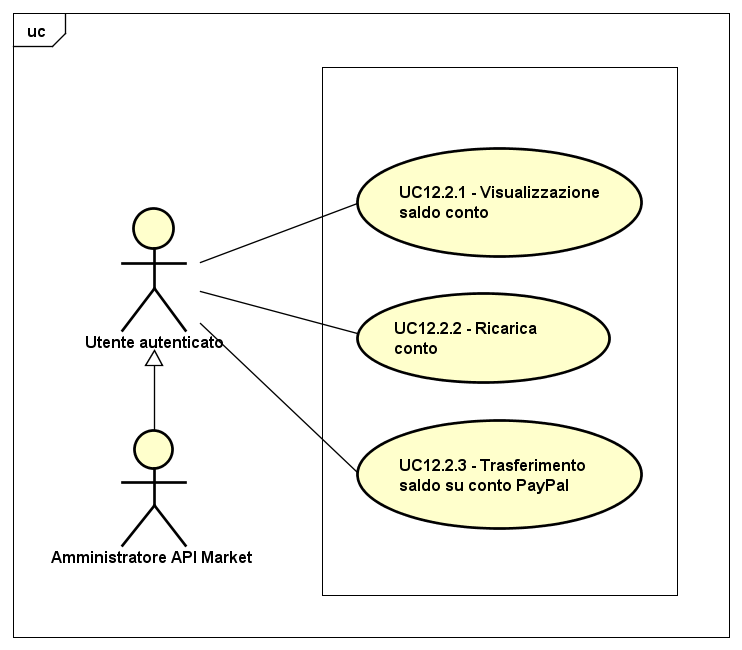
\includegraphics[scale=0.45]{UML/UC12_2.png}
	\caption{UC12.2: Gestione conto personale}
\end{figure}

\begin{minipage}{\linewidth}
	\begin{tabular}{ l | p{11cm}}
		\hline
		\rowcolor{Gray}
		\multicolumn{2}{c}{UC12.2 - Gestione conto personale} \\
		\hline
		\textbf{Attori} & Cliente \\
		\textbf{Descrizione} & L'attore visualizza le informazioni del proprio conto utente e/o effettua una ricarica su di esso \\
		\textbf{Pre-Condizioni} & L'attore si trova nella schermata relativa alla gestione del proprio profilo utente \\
		\textbf{Post-Condizioni} & L'attore ha visualizzato il saldo del proprio conto utente e/o effettuato una ricarica su di esso \\
		\textbf{Scenario Principale} & 
		\begin{enumerate*}[label=(\arabic*.),itemjoin={\newline}]
			\item L'attore può visualizzare il saldo corrente del proprio conto utente (UC12.2.1)
			\item L'attore può effettuare una ricarica sul proprio conto utente (UC12.2.2)
		\end{enumerate*}
	\end{tabular}
\end{minipage}

\paragraph{Caso d'uso UC12.2.1: Visualizzazione saldo conto}
\label{UC12_2_1}

\begin{minipage}{\linewidth}
	\begin{tabular}{ l | p{11cm}}
		\hline
		\rowcolor{Gray}
		\multicolumn{2}{c}{UC12.2.1 - Visualizzazione saldo conto} \\
		\hline
		\textbf{Attori} & Cliente \\
		\textbf{Descrizione} & L'attore visualizza il saldo corrente del proprio conto utente \\
		\textbf{Pre-Condizioni} & L'attore si trova nella schermata relativa alla gestione del proprio conto utente \\
		\textbf{Post-Condizioni} & L'attore ha visualizzato il saldo corrente del proprio conto utente \\
		\textbf{Scenario Principale} & 
		\begin{enumerate*}[label=(\arabic*.),itemjoin={\newline}]
			\item L'attore può visualizzare il saldo corrente del proprio conto utente
		\end{enumerate*}\\
	\end{tabular}
\end{minipage}

\paragraph{Caso d'uso UC12.2.2: Ricarica conto}
\label{UC12_2_2}
\begin{figure}[ht]
	\centering
	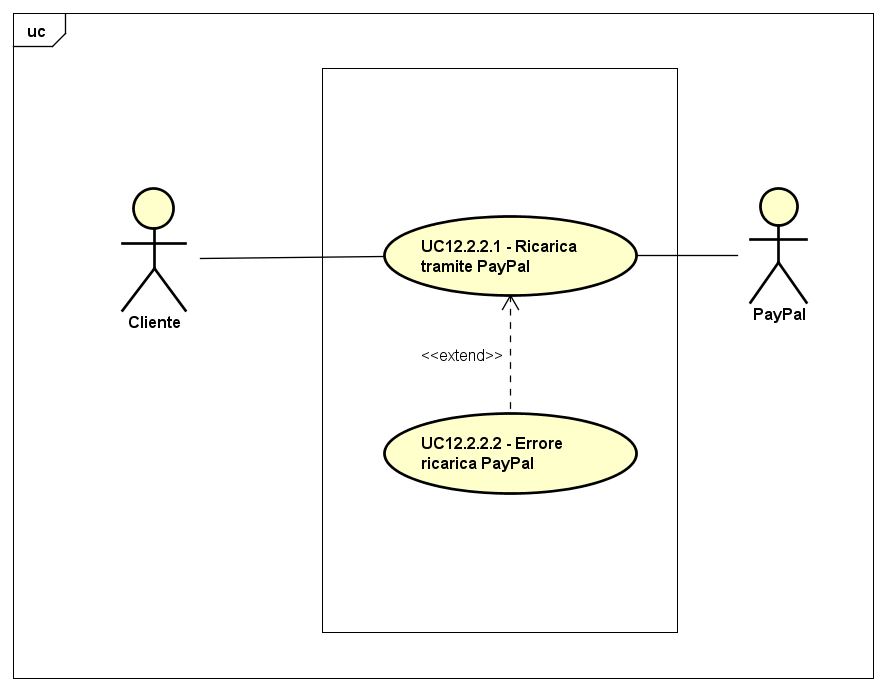
\includegraphics[scale=0.45]{UML/UC12_2_2.png}
	\caption{UC12.2.2: Ricarica conto}
\end{figure}

\begin{minipage}{\linewidth}
	\begin{tabular}{ l | p{11cm}}
		\hline
		\rowcolor{Gray}
		\multicolumn{2}{c}{UC12.2.2 - Ricarica conto} \\
		\hline
		\textbf{Attori} & Cliente, PayPal \\
		\textbf{Descrizione} & L'attore effettua una ricarica sul proprio conto utente \\
		\textbf{Pre-Condizioni} & L'attore si trova nella schermata relativa alla gestione del proprio conto utente \\
		\textbf{Post-Condizioni} & L'attore ha effettuato una ricarica sul proprio conto utente \\
		\textbf{Scenario Principale} & 
		\begin{enumerate*}[label=(\arabic*.),itemjoin={\newline}]
			\item L'attore può effettuare una ricarica tramite PayPal sul proprio conto utente (UC12.2.2.1)
		\end{enumerate*}\\
		\textbf{Scenari Alternativi} & 
		\begin{enumerate*}[label=(\arabic*.),itemjoin={\newline}]
			\item L'attore può visualizzare un messaggio di errore informativo (E.g: dati errati), e la ricarica tramite PayPal sul proprio conto utente non avviene (UC12.2.2.2)
		\end{enumerate*}\\
	\end{tabular}
\end{minipage}

\subparagraph{Caso d'uso UC12.2.2.1: Ricarica tramite PayPal}
\label{UC12_2_2_1}

\begin{minipage}{\linewidth}
	\begin{tabular}{ l | p{11cm}}
		\hline
		\rowcolor{Gray}
		\multicolumn{2}{c}{UC12.2.2.1 - Ricarica tramite PayPal} \\
		\hline
		\textbf{Attori} & Cliente, PayPal \\
		\textbf{Descrizione} & L'attore effettua una ricarica tramite PayPal sul proprio conto utente \\
		\textbf{Pre-Condizioni} & L'attore si trova nella schermata relativa alla ricarica del proprio conto utente \\
		\textbf{Post-Condizioni} & L'attore ha effettuato una ricarica tramite PayPal sul proprio conto utente \\
		\textbf{Scenario Principale} & 
		\begin{enumerate*}[label=(\arabic*.),itemjoin={\newline}]
			\item L'attore può effettuare una ricarica tramite PayPal sul proprio conto utente
		\end{enumerate*}\\
	\end{tabular}
\end{minipage}

\subparagraph{Caso d'uso UC12.2.2.2: Errore ricarica PayPal}
\label{UC12_2_2_2}

\begin{minipage}{\linewidth}
	\begin{tabular}{ l | p{11cm}}
		\hline
		\rowcolor{Gray}
		\multicolumn{2}{c}{UC12.2.2.2 - Errore ricarica PayPal} \\
		\hline
		\textbf{Attori} & Cliente, PayPal \\
		\textbf{Descrizione} & L'attore visualizza un messaggio di errore informativo e la ricarica tramite PayPal sul proprio conto utente non avviene \\
		\textbf{Pre-Condizioni} & L'attore ha confermato la ricarica tramite PayPal sul proprio conto utente ma si è verificato un errore \\
		\textbf{Post-Condizioni} & L'attore ha visualizzato un messaggio di errore informativo \\
		\textbf{Scenario Principale} & 
		\begin{enumerate*}[label=(\arabic*.),itemjoin={\newline}]
			\item L'attore può visualizzare un messaggio di errore informativo e la ricarica tramite PayPal sul proprio conto utente non avviene
		\end{enumerate*}\\
	\end{tabular}
\end{minipage}

\newpage
\subsubsection{Caso d'uso UC12.3: Visualizzazione storico transazioni}
\label{UC12_3}
\begin{figure}[ht]
	\centering
	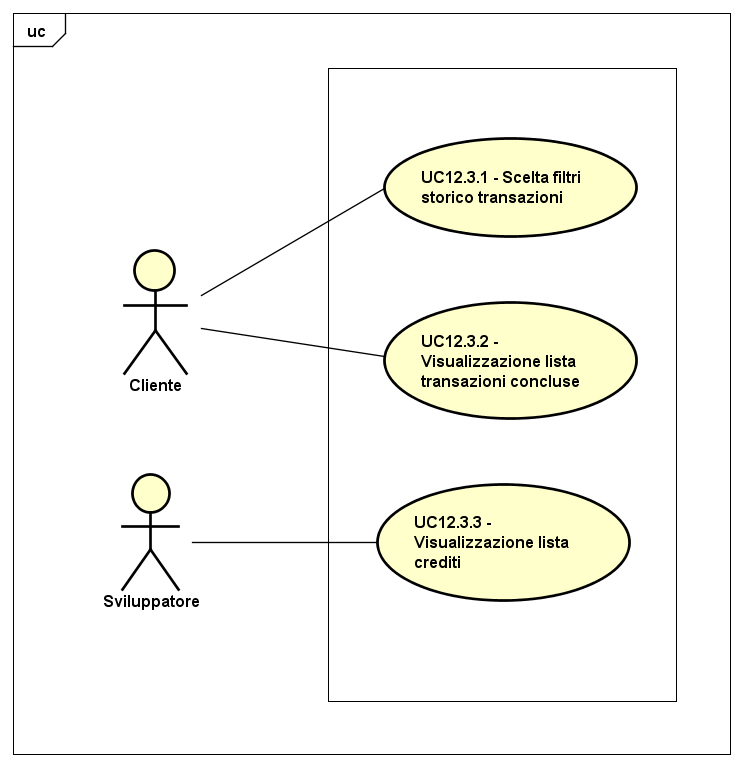
\includegraphics[scale=0.45]{UML/UC12_3.png}
	\caption{UC12.3: Visualizzazione storico transazioni}
\end{figure}

\begin{minipage}{\linewidth}
	\begin{tabular}{ l | p{11cm}}
		\hline
		\rowcolor{Gray}
		\multicolumn{2}{c}{UC12.3 - Visualizzazione storico transazioni} \\
		\hline
		\textbf{Attori} & Cliente, Sviluppatore \\
		\textbf{Descrizione} & L'attore visualizza lo storico delle proprie transazioni \\
		\textbf{Pre-Condizioni} & L'attore si trova nella schermata relativa alla gestione del proprio profilo utente \\
		\textbf{Post-Condizioni} & L'attore ha visualizzato lo storico delle proprie transazioni \\
		\textbf{Scenario Principale} & 
		\begin{enumerate*}[label=(\arabic*.),itemjoin={\newline}]
			\item L'attore può scegliere i filtri di visualizzazione (UC12.3.1)
			\item L'attore può visualizzare la lista delle proprie transazioni concluse (UC12.3.2)
			\item Lo sviluppatore può visualizzare la lista dei propri crediti (UC12.3.3)
		\end{enumerate*}
	\end{tabular}
\end{minipage}

\newpage
\paragraph{Caso d'uso UC12.3.1: Scelta filtri storico transazioni}
\label{UC12_3_1}
\begin{figure}[ht]
	\centering
	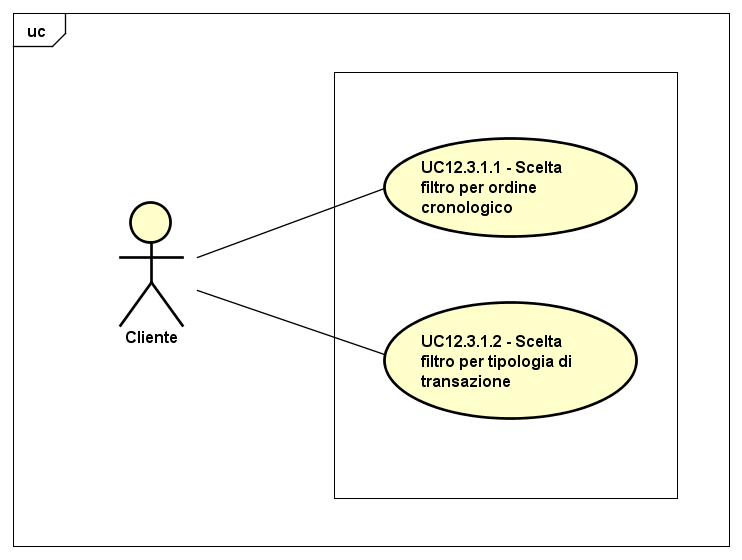
\includegraphics[scale=0.45]{UML/UC12_3_1.png}
	\caption{UC12.3.1: Scelta filtri storico transazioni}
\end{figure}

\begin{minipage}{\linewidth}
	\begin{tabular}{ l | p{11cm}}
		\hline
		\rowcolor{Gray}
		\multicolumn{2}{c}{UC12.3.1 - Scelta filtri storico transazioni} \\
		\hline
		\textbf{Attori} & Cliente \\
		\textbf{Descrizione} & L'attore scegliere i filtri per lo storico delle proprie transazioni \\
	\textbf{Pre-Condizioni} & L'attore si trova nella schermata relativa alla visualizzazione dello storico delle proprie transazioni \\
	\textbf{Post-Condizioni} & L'attore ha scelto i filtri per lo storico delle proprie transazioni \\
	\textbf{Scenario Principale} & 
	\begin{enumerate*}[label=(\arabic*.),itemjoin={\newline}]
		\item L'attore può scegliere il filtro per ordine cronologico (UC12.3.1.1)
		\item L'attore può scegliere il filtro per tipologia di transazione (UC12.3.1.2)
	\end{enumerate*}
	\end{tabular}
\end{minipage}

\subparagraph{Caso d'uso UC12.3.1.1: Scelta filtro per ordine cronologico}
\label{UC12_3_1_1}

\begin{minipage}{\linewidth}
	\begin{tabular}{ l | p{11cm}}
		\hline
		\rowcolor{Gray}
		\multicolumn{2}{c}{UC12.3.1.1 - Scelta filtro per ordine cronologico} \\
		\hline
		\textbf{Attori} & Cliente \\
		\textbf{Descrizione} & L'attore sceglie il filtro per ordine cronologico \\
	\textbf{Pre-Condizioni} & L'attore si trova nella schermata relativa alla visualizzazione dello storico delle proprie transazioni \\
	\textbf{Post-Condizioni} & L'attore ha scelto il filtro per ordine cronologico \\
	\textbf{Scenario Principale} & 
	\begin{enumerate*}[label=(\arabic*.),itemjoin={\newline}]
		\item L'attore può scegliere il filtro per ordine cronologico
	\end{enumerate*}
	\end{tabular}
\end{minipage}

\subparagraph{Caso d'uso UC12.3.1.2: Scelta filtro per tipologia di transazione}
\label{UC12_3_1_2}

\begin{minipage}{\linewidth}
	\begin{tabular}{ l | p{11cm}}
		\hline
		\rowcolor{Gray}
		\multicolumn{2}{c}{UC12.3.1.2 - Scelta filtro per tipologia di transazione} \\
		\hline
		\textbf{Attori} & Cliente \\
		\textbf{Descrizione} & L'attore sceglie il filtro per tipologia di transazione \\
	\textbf{Pre-Condizioni} & L'attore si trova nella schermata relativa alla visualizzazione dello storico delle proprie transazioni \\
	\textbf{Post-Condizioni} & L'attore ha scelto il filtro per tipologia di transazione \\
	\textbf{Scenario Principale} & 
	\begin{enumerate*}[label=(\arabic*.),itemjoin={\newline}]
		\item L'attore può scegliere il filtro per tipologia di transazione
	\end{enumerate*}
	\end{tabular}
\end{minipage}

\newpage
\paragraph{Caso d'uso UC12.3.2: Visualizzazione lista transazioni concluse}
\label{UC12_3_2}
\begin{figure}[ht]
	\centering
	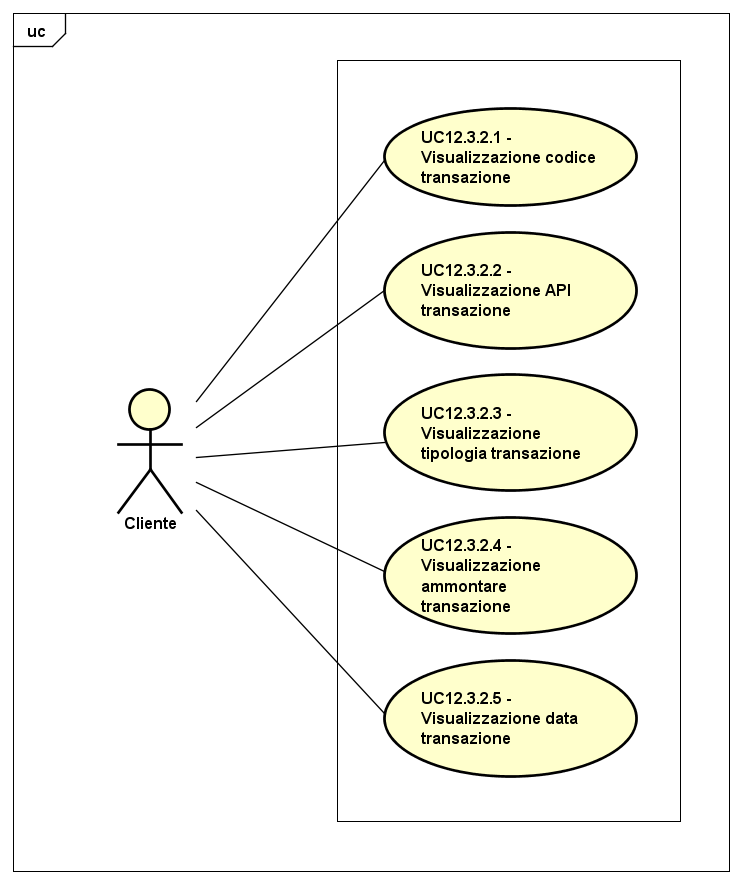
\includegraphics[scale=0.45]{UML/UC12_3_2.png}
	\caption{UC12.3.2: Visualizzazione lista transazioni concluse}
\end{figure}

\begin{minipage}{\linewidth}
	\begin{tabular}{ l | p{11cm}}
		\hline
		\rowcolor{Gray}
		\multicolumn{2}{c}{UC12.3.2 - Visualizzazione lista transazioni concluse} \\
		\hline
		\textbf{Attori} & Cliente \\
		\textbf{Descrizione} & L'attore visualizza la lista delle proprie transazioni \\
		\textbf{Pre-Condizioni} & L'attore si trova nella schermata relativa alla visualizzazione dello storico delle proprie transazioni \\
		\textbf{Post-Condizioni} & L'attore ha visualizzato la lista delle proprie transazioni \\
		\textbf{Scenario Principale} & 
		\begin{enumerate*}[label=(\arabic*.),itemjoin={\newline}]
			\item L'attore può visualizzare il codice della transazione (UC12.3.2.1)
			\item L'attore può visualizzare l'API di riferimento alla transazione (UC12.3.2.2)
			\item L'attore può visualizzare la tipologia della transazione (UC12.3.2.3)
			\item L'attore può visualizzare l'ammontare del denaro coinvolto nella transazione (UC12.3.2.4)
			\item L'attore può visualizzare la data della transazione (UC12.3.2.5)
		\end{enumerate*}\\
	\end{tabular}
\end{minipage}

\subparagraph{Caso d'uso UC12.3.2.1: Visualizzazione codice transazione}
\label{UC12_3_2_1}

\begin{minipage}{\linewidth}
	\begin{tabular}{ l | p{11cm}}
		\hline
		\rowcolor{Gray}
		\multicolumn{2}{c}{UC12.3.2.1 - Visualizzazione codice transazione} \\
		\hline
		\textbf{Attori} & Cliente \\
		\textbf{Descrizione} & L'attore visualizza il codice della propria transazione \\
	\textbf{Pre-Condizioni} & L'attore si trova nella schermata relativa alla visualizzazione dello storico delle proprie transazioni \\
	\textbf{Post-Condizioni} & L'attore ha visualizzato il codice della propria transazione \\
	\textbf{Scenario Principale} & 
	\begin{enumerate*}[label=(\arabic*.),itemjoin={\newline}]
		\item L'attore può visualizzare il codice della propria transazione
	\end{enumerate*}
	\end{tabular}
\end{minipage}

\subparagraph{Caso d'uso UC12.3.2.2: Visualizzazione API transazione}
\label{UC12_3_2_2}

\begin{minipage}{\linewidth}
	\begin{tabular}{ l | p{11cm}}
		\hline
		\rowcolor{Gray}
		\multicolumn{2}{c}{UC12.3.2.2 - Visualizzazione API transazione} \\
		\hline
		\textbf{Attori} & Cliente \\
		\textbf{Descrizione} & L'attore visualizza l'API di riferimento alla propria transazione \\
	\textbf{Pre-Condizioni} & L'attore si trova nella schermata relativa alla visualizzazione dello storico delle proprie transazioni \\
	\textbf{Post-Condizioni} & L'attore ha visualizzato l'API di riferimento alla propria transazione \\
	\textbf{Scenario Principale} & 
	\begin{enumerate*}[label=(\arabic*.),itemjoin={\newline}]
		\item L'attore può visualizzare l'API di riferimento alla propria transazione
	\end{enumerate*}
	\end{tabular}
\end{minipage}

\subparagraph{Caso d'uso UC12.3.2.3: Visualizzazione tipologia transazione}
\label{UC12_3_2_3}

\begin{minipage}{\linewidth}
	\begin{tabular}{ l | p{11cm}}
		\hline
		\rowcolor{Gray}
		\multicolumn{2}{c}{UC12.3.2.3 - Visualizzazione tipologia transazione} \\
		\hline
		\textbf{Attori} & Cliente \\
		\textbf{Descrizione} & L'attore visualizza la tipologia della propria transazione \\
	\textbf{Pre-Condizioni} & L'attore si trova nella schermata relativa alla visualizzazione dello storico delle proprie transazioni \\
	\textbf{Post-Condizioni} & L'attore ha visualizzato la tipologia della propria transazione \\
	\textbf{Scenario Principale} & 
	\begin{enumerate*}[label=(\arabic*.),itemjoin={\newline}]
		\item L'attore può visualizzare la tipologia della propria transazione
	\end{enumerate*}
	\end{tabular}
\end{minipage}

\subparagraph{Caso d'uso UC12.3.2.4: Visualizzazione ammontare transazione}
\label{UC12_3_2_4}

\begin{minipage}{\linewidth}
	\begin{tabular}{ l | p{11cm}}
		\hline
		\rowcolor{Gray}
		\multicolumn{2}{c}{UC12.3.2.4 - Visualizzazione ammontare transazione} \\
		\hline
		\textbf{Attori} & Cliente \\
		\textbf{Descrizione} & L'attore visualizza l'ammontare coinvolto nella propria transazione \\
	\textbf{Pre-Condizioni} & L'attore si trova nella schermata relativa alla visualizzazione dello storico delle proprie transazioni \\
	\textbf{Post-Condizioni} & L'attore ha visualizzato l'ammontare coinvolto nella propria transazione propria transazione \\
	\textbf{Scenario Principale} & 
	\begin{enumerate*}[label=(\arabic*.),itemjoin={\newline}]
		\item L'attore può visualizzare l'ammontare coinvolto nella propria transazione propria transazione
	\end{enumerate*}
	\end{tabular}
\end{minipage}

\subparagraph{Caso d'uso UC12.3.2.5: Visualizzazione data transazione}
\label{UC12_3_2_5}

\begin{minipage}{\linewidth}
	\begin{tabular}{ l | p{11cm}}
		\hline
		\rowcolor{Gray}
		\multicolumn{2}{c}{UC12.3.2.5 - Visualizzazione data transazione} \\
		\hline
		\textbf{Attori} & Cliente \\
		\textbf{Descrizione} & L'attore visualizza la data della propria transazione \\
	\textbf{Pre-Condizioni} & L'attore si trova nella schermata relativa alla visualizzazione dello storico delle proprie transazioni \\
	\textbf{Post-Condizioni} & L'attore ha visualizzato la data della propria transazione \\
	\textbf{Scenario Principale} & 
	\begin{enumerate*}[label=(\arabic*.),itemjoin={\newline}]
		\item L'attore può visualizzare la data della propria transazione
	\end{enumerate*}
	\end{tabular}
\end{minipage}

\newpage
\paragraph{Caso d'uso UC12.3.3: Visualizzazione lista credito}
\label{UC12_3_3}
\begin{figure}[ht]
	\centering
	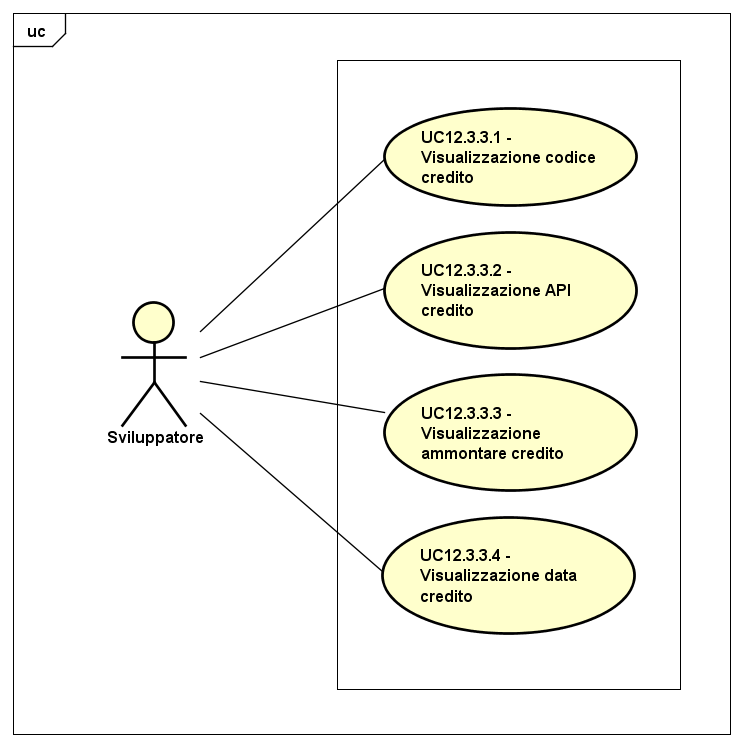
\includegraphics[scale=0.45]{UML/UC12_3_3.png}
	\caption{UC12.3.3: Visualizzazione lista credito}
\end{figure}

\begin{minipage}{\linewidth}
	\begin{tabular}{ l | p{11cm}}
		\hline
		\rowcolor{Gray}
		\multicolumn{2}{c}{UC12.3.3 - Visualizzazione lista credito} \\
		\hline
		\textbf{Attori} & Sviluppatore \\
		\textbf{Descrizione} & L'attore visualizza la lista dei propri crediti \\
		\textbf{Pre-Condizioni} & L'attore si trova nella schermata relativa alla visualizzazione dello storico delle proprie transazioni \\
		\textbf{Post-Condizioni} & L'attore ha visualizzato la lista dei propri crediti \\
		\textbf{Scenario Principale} & 
		\begin{enumerate*}[label=(\arabic*.),itemjoin={\newline}]
			\item L'attore può visualizzare il codice del credito (UC12.3.3.1)
			\item L'attore può visualizzare l'API di riferimento al credito (UC12.3.3.2)
			\item L'attore può visualizzare l'ammontare del credito accumulato per l'API di riferimento (UC12.3.3.3)
			\item L'attore può visualizzare la data del credito (UC12.3.3.4)
		\end{enumerate*}\\
	\end{tabular}
\end{minipage}

\subparagraph{Caso d'uso UC12.3.3.1: Visualizzazione codice credito}
\label{UC12_3_3_1}

\begin{minipage}{\linewidth}
	\begin{tabular}{ l | p{11cm}}
		\hline
		\rowcolor{Gray}
		\multicolumn{2}{c}{UC12.3.3.1 - Visualizzazione codice credito} \\
		\hline
		\textbf{Attori} & Sviluppatore \\
		\textbf{Descrizione} & L'attore visualizza il codice del proprio credito \\
	\textbf{Pre-Condizioni} & L'attore si trova nella schermata relativa alla visualizzazione dello storico delle proprie transazioni \\
	\textbf{Post-Condizioni} & L'attore ha visualizzato il codice del proprio credito \\
	\textbf{Scenario Principale} & 
	\begin{enumerate*}[label=(\arabic*.),itemjoin={\newline}]
		\item L'attore può visualizzare il codice del proprio credito
	\end{enumerate*}
	\end{tabular}
\end{minipage}

\subparagraph{Caso d'uso UC12.3.3.2: Visualizzazione API credito}
\label{UC12_3_3_2}

\begin{minipage}{\linewidth}
	\begin{tabular}{ l | p{11cm}}
		\hline
		\rowcolor{Gray}
		\multicolumn{2}{c}{UC12.3.3.2 - Visualizzazione API credito} \\
		\hline
		\textbf{Attori} & Sviluppatore \\
		\textbf{Descrizione} & L'attore visualizza l'API di riferimento al proprio credito \\
	\textbf{Pre-Condizioni} & L'attore si trova nella schermata relativa alla visualizzazione dello storico delle proprie transazioni \\
	\textbf{Post-Condizioni} & L'attore ha visualizzato l'API di riferimento al proprio credito \\
	\textbf{Scenario Principale} & 
	\begin{enumerate*}[label=(\arabic*.),itemjoin={\newline}]
		\item L'attore può visualizzare l'API di riferimento al proprio credito
	\end{enumerate*}
	\end{tabular}
\end{minipage}
	
\subparagraph{Caso d'uso UC12.3.3.3: Visualizzazione ammontare credito}
\label{UC12_3_3_3}

\begin{minipage}{\linewidth}
	\begin{tabular}{ l | p{11cm}}
		\hline
		\rowcolor{Gray}
		\multicolumn{2}{c}{UC12.3.3.3 - Visualizzazione ammontare credito} \\
		\hline
		\textbf{Attori} & Sviluppatore \\
		\textbf{Descrizione} & L'attore visualizza l'ammontare del proprio credito per l'API di riferimento \\
	\textbf{Pre-Condizioni} & L'attore si trova nella schermata relativa alla visualizzazione dello storico delle proprie transazioni \\
	\textbf{Post-Condizioni} & L'attore ha visualizzato ll'ammontare del proprio credito per l'API di riferimento \\
	\textbf{Scenario Principale} & 
	\begin{enumerate*}[label=(\arabic*.),itemjoin={\newline}]
		\item L'attore può visualizzare l'ammontare del proprio credito per l'API di riferimento
	\end{enumerate*}
	\end{tabular}
\end{minipage}

\subparagraph{Caso d'uso UC12.3.3.4: Visualizzazione data credito}
\label{UC12_3_3_4}

\begin{minipage}{\linewidth}
	\begin{tabular}{ l | p{11cm}}
		\hline
		\rowcolor{Gray}
		\multicolumn{2}{c}{UC12.3.3.4 - Visualizzazione data credito} \\
		\hline
		\textbf{Attori} & Sviluppatore \\
		\textbf{Descrizione} & L'attore visualizza la data del proprio credito per l'API di riferimento \\
	\textbf{Pre-Condizioni} & L'attore si trova nella schermata relativa alla visualizzazione dello storico delle proprie transazioni \\
	\textbf{Post-Condizioni} & L'attore ha visualizzato la data del proprio credito per l'API di riferimento \\
	\textbf{Scenario Principale} & 
	\begin{enumerate*}[label=(\arabic*.),itemjoin={\newline}]
		\item L'attore può visualizzare la data del proprio credito per l'API di riferimento
	\end{enumerate*}
	\end{tabular}
\end{minipage}
\newpage
\subsection{Caso d'uso UC13: Logout}
\label{UC13}

\begin{longtable}{ l | p{11cm}}
	\hline
	\rowcolor{Gray}
	\multicolumn{2}{c}{UC13 - Logout} \\
	\hline
	\textbf{Attori} & Utente autenticato, Amministratore API Market \\
	\textbf{Descrizione} & L'attore effettua il logout, retrocedendo ad un utente non autenticato e venendo reindirizzato alla schermata iniziale \\
	\textbf{Pre-Condizioni} & L'attore si trova nella schermata iniziale dell'applicazione web \\
	\textbf{Post-Condizioni}& L'attore ha effettuato il logout, è stato retrocesso ad un utente non autenticato e reindirizzato alla schermata iniziale \\
	\textbf{Scenario Principale} & 
	\begin{enumerate*}[label=(\arabic*.),itemjoin={\newline}]
		\item L'attore può effettuare il logout, retrocedendo ad un utente non autenticato e venendo reindirizzato alla schermata iniziale (UC1)
	\end{enumerate*}\\
\end{longtable}
\newpage
\subsection{Caso d'uso UC14: Amministrazione applicazione web}
\label{UC14}
\begin{figure}[ht]
	\centering
	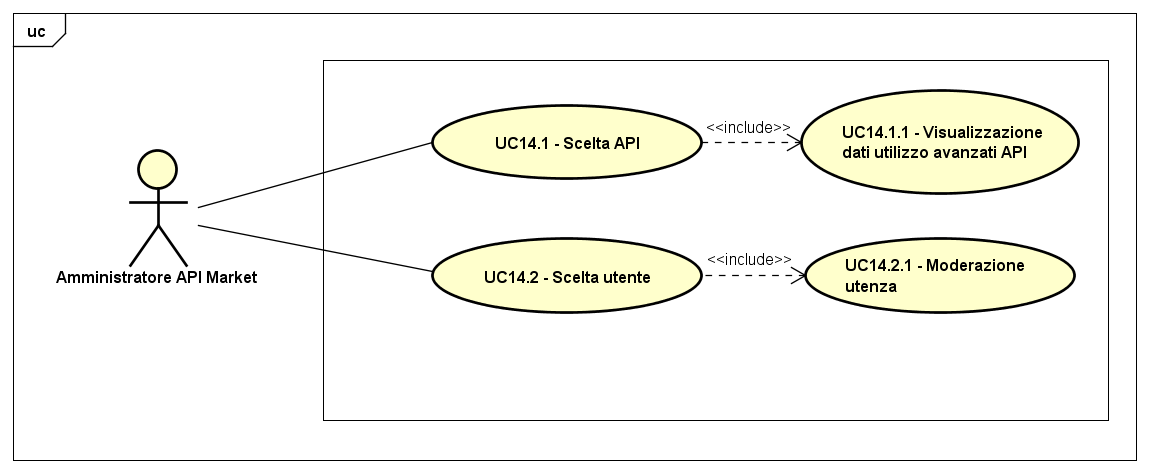
\includegraphics[scale=0.45]{UML/UC14.png}
	\caption{UC14: Amministrazione applicazione web}
\end{figure}

\renewcommand*{\arraystretch}{1.6}
\begin{longtable}{ l | p{11cm}}
	\hline
	\rowcolor{Gray}
	\multicolumn{2}{c}{UC14: Amministrazione applicazione web} \\
	\hline
	\textbf{Attori} & Amministratore API Market \\
	\textbf{Descrizione} & L'attore può gestire la parte riservata della piattaforma, ed effettuare operazioni super-user su utenza, prodotti registrati e sulla piattaforma stessa \\
	\textbf{Pre-Condizioni} & L'attore visita la pagina relativa all'amministrazione della piattaforma API Market\\
	\textbf{Post-Condizioni}& L'attore ha effettuato le modifiche desiderate, o ha consultato i dati desiderati, all'interno della piattaforma\\
	\textbf{Scenario Principale} & \begin{enumerate*}[label=(\arabic*.),itemjoin={\newline}]
		\item L'attore può consultare i dati di utilizzo avanzati per un API (UC14.1)
		\item L'attore può moderare l'utenza predisponendo sospensioni (UC14.2)
	\end{enumerate*}\\
\end{longtable}


\subsubsection{Caso d'uso UC14.1: Visualizzazione dati di utilizzo avanzati}
\label{UC14_1}

\begin{minipage}{\linewidth}
	\begin{tabular}{ l | p{11cm}}
		\hline
		\rowcolor{Gray}
		\multicolumn{2}{c}{UC14.1 - Visualizzazione dati di utilizzo avanzati} \\
		\hline
		\textbf{Attori} &  Amministratore API Market \\
		\textbf{Descrizione} & L'attore visualizza nella schermata relativa ai dati di utilizzo dell'API \\
		\textbf{Pre-Condizioni} & L'attore ha selezionato la visualizzazione dati per un API \\
		\textbf{Post-Condizioni} & L'attore ha visualizzato i dati di utilizzo avanzati dell'API selezionata \\
		\textbf{Scenario Principale} & 
		\begin{enumerate*}[label=(\arabic*.),itemjoin={\newline}]
			\item L'attore può visualizzare il numero di licenze attive per l'API selezionata (UC7.7.1)
			\item L'attore può visualizzare il numero di chiamate giornaliere effettuate all'API selezionata (UC7.7.2)
			\item L'attore può visualizzare il tempo medio di utilizzo dell'API selezionata (UC7.7.3)
			\item L'attore può visualizzare il traffico medio giornaliero dell'API selezionata (UC7.7.4)
			\item L'attore può visualizzare la lista di utenti che hanno una licenza attiva (UC14.1.1)
			\item L'attore può visualizzare il tempo medio di risposta (UC14.1.2)
		\end{enumerate*}\\
	\end{tabular}
\end{minipage}

\paragraph{Caso d'uso UC14.1.1: Visualizzazione utenti attivi per API}
\label{UC14_1_1}

\begin{minipage}{\linewidth}
	\begin{tabular}{ l | p{11cm}}
		\hline
		\rowcolor{Gray}
		\multicolumn{2}{c}{UC14.1.1 - Visualizzazione utenti attivi per API} \\
		\hline
		\textbf{Attori} & Amministratore API Market \\
		\textbf{Descrizione} & L'attore visualizza una lista di utenti attivi per l'API selezionata \\
		\textbf{Pre-Condizioni} & L'attore ha selezionato un API per il quale visualizzare i dati di utilizzo avanzati\\
		\textbf{Post-Condizioni} & L'attore ha visualizzato la lista di licenze attive per l'API selezionata \\
		\textbf{Scenario Principale} & 
		\begin{enumerate*}[label=(\arabic*.),itemjoin={\newline}]
			\item L'attore può visualizzare il nome dell'utente (UC14.1.1.1)
			\item L'attore può visualizzare la durata della licenza (UC14.1.1.2)
		\end{enumerate*}\\
	\end{tabular}
\end{minipage}

\subparagraph{Caso d'uso UC14.1.1.1: Visualizzazione nome}
\label{UC14_1_1_1}

\begin{minipage}{\linewidth}
	\begin{tabular}{ l | p{11cm}}
		\hline
		\rowcolor{Gray}
		\multicolumn{2}{c}{UC14.1.1.1 - Visualizzazione nome} \\
		\hline
		\textbf{Attori} & Amministratore API Market \\
		\textbf{Descrizione} & L'attore può visualizzare il nome dell'utente interessato\\
		\textbf{Pre-Condizioni} & L'attore è nella schermata di visualizzazione degli utenti con licenza attiva per l'API selezionata\\
		\textbf{Post-Condizioni} & L'attore ha visualizzato il nome interessato \\
		\textbf{Scenario Principale} & 
		\begin{enumerate*}[label=(\arabic*.),itemjoin={\newline}]
			\item L'attore può visualizzare il nome dell'utente corrispondente
		\end{enumerate*}
	\end{tabular}
\end{minipage}

\subparagraph{Caso d'uso UC14.1.1.2: Visualizzazione durata residua licenza}
\label{UC14_1_1_2}

\begin{minipage}{\linewidth}
	\begin{tabular}{ l | p{11cm}}
		\hline
		\rowcolor{Gray}
		\multicolumn{2}{c}{UC14.1.1.2 -  Visualizzazione durata residua licenza} \\
		\hline
		\textbf{Attori} & Amministratore API Market \\
		\textbf{Descrizione} & L'attore può visualizzare la durata residua della licenza dell'utente interessato\\
		\textbf{Pre-Condizioni} & L'attore è nella schermata di visualizzazione degli utenti con licenza attiva per l'API selezionata\\
		\textbf{Post-Condizioni} & L'attore ha visualizzato la data di scadenza \\
		\textbf{Scenario Principale} & 
		\begin{enumerate*}[label=(\arabic*.),itemjoin={\newline}]
			\item L'attore può visualizzare la scadenza per l'utente visualizzato riguardante l'API selezionata
		\end{enumerate*}
	\end{tabular}
\end{minipage}

\paragraph{Caso d'uso UC14.1.2: Visualizzazione tempo medio di risposta}
\label{UC14_1_2}

\begin{minipage}{\linewidth}
	\begin{tabular}{ l | p{11cm}}
		\hline
		\rowcolor{Gray}
		\multicolumn{2}{c}{UC14.1.2 - Visualizzazione tempo medio di risposta} \\
		\hline
		\textbf{Attori} & Amministratore API Market \\
		\textbf{Descrizione} & L'attore visualizza il tempo medio di risposta per l'API selezionata \\
		\textbf{Pre-Condizioni} & L'attore ha selezionato un API per il quale visualizzare i dati di utilizzo avanzati\\
		\textbf{Post-Condizioni} & L'attore ha visualizzato il tempo medio di risposta per l'API selezionata \\
		\textbf{Scenario Principale} & 
		\begin{enumerate*}[label=(\arabic*.),itemjoin={\newline}]
			\item L'attore può visualizzare il tempo medio di risposta per l'API selezionata
		\end{enumerate*}\\
	\end{tabular}
\end{minipage}

\subsubsection{Caso d'uso UC14.2: Azioni utente}
\label{UC14_2}

\begin{minipage}{\linewidth}
	\begin{tabular}{ l | p{11cm}}
		\hline
		\rowcolor{Gray}
		\multicolumn{2}{c}{UC14.2 - Azioni utente} \\
		\hline
		\textbf{Attori} &  Amministratore API Market \\
		\textbf{Descrizione} & L'attore visualizza nella schermata relativa ai dati di utilizzo dell'API \\
		\textbf{Pre-Condizioni} & L'attore ha selezionato la visualizzazione dati per un API \\
		\textbf{Post-Condizioni} & L'attore ha visualizzato i dati di utilizzo avanzati dell'API selezionata \\
		\textbf{Scenario Principale} & 
		\begin{enumerate*}[label=(\arabic*.),itemjoin={\newline}]
			\item L'attore può inserire il nome di un utente su cui effettuare un azione (UC14.2.1)
			\item L'attore può sospendere l'utente selezionato (UC14.2.2)
			\item L'attore può sospendere i prelievi di denaro dal proprio conto per l'utente selezionato (UC14.2.3)
			\item L'attore può rimuovere una sospensione utente (UC14.2.4)
			\item L'attore può rimuovere la sospensione dei prelievi (UC14.2.5)
		\end{enumerate*}\\
		\textbf{Scenari Alternativi} & 
		\begin{enumerate*}[label=(\arabic*.),itemjoin={\newline}]
			\item L'attore riceve un messaggio d'errore qualora l'utente inserito non esista. Può dunque ritentare la procedura
		\end{enumerate*}\\
	\end{tabular}
\end{minipage}

\paragraph{Caso d'uso UC14.2.1: Inserimento username}
\label{UC14_2_1}

\begin{minipage}{\linewidth}
	\begin{tabular}{ l | p{11cm}}
		\hline
		\rowcolor{Gray}
		\multicolumn{2}{c}{UC14.2.1 - Inserimento username} \\
		\hline
		\textbf{Attori} & Amministratore API Market \\
		\textbf{Descrizione} & L'attore inserisce l'username di un utente sul quale effettuare operazioni \\
		\textbf{Pre-Condizioni} & L'attore ha scelto di effettuare azioni su un utente\\
		\textbf{Post-Condizioni} & L'attore ha inserito il nome di un utente \\
		\textbf{Scenario Principale} & 
		\begin{enumerate*}[label=(\arabic*.),itemjoin={\newline}]
			\item L'attore può inserire il nome di un utente
		\end{enumerate*}\\
	\end{tabular}
\end{minipage}

\paragraph{Caso d'uso UC14.2.2: Sospensione utente}
\label{UC14_2_2}

\begin{minipage}{\linewidth}
	\begin{tabular}{ l | p{11cm}}
		\hline
		\rowcolor{Gray}
		\multicolumn{2}{c}{UC14.2.2 - Sospensione utente} \\
		\hline
		\textbf{Attori} & Amministratore API Market \\
		\textbf{Descrizione} & L'attore può sospendere l'utente indicato \\
		\textbf{Pre-Condizioni} & L'attore ha inserito il nome utente da sospendere\\
		\textbf{Post-Condizioni} & L'attore ha sospeso un utente \\
		\textbf{Scenario Principale} & 
		\begin{enumerate*}[label=(\arabic*.),itemjoin={\newline}]
			\item L'attore può inserire la durata in giorni della sospensione (UC14.2.2.1)
			\item L'attore può confermare la scelta (UC14.2.2.2)
		\end{enumerate*}\\
	\end{tabular}
\end{minipage}

\newpage
\textbf{Da fare: UC14.2.3 e sottocasi, UC14.2.4 e sottocasi, UC14.2.5 e sottocasi, UC14.2.2.1, UC14.2.2.2}

